\documentclass[letterpaper,12pt]{report}
\usepackage[spanish]{babel}
\usepackage[utf8]{inputenc}
\usepackage{graphicx}
\usepackage{amsfonts,amsmath,color,amssymb,float, amsthm,mathrsfs}  
\usepackage[right=3cm,left=2cm,top=2cm,bottom=2cm,headsep=0.7cm,footskip=0.5cm]{geometry}
\usepackage{enumerate}
\usepackage{wrapfig} 
\usepackage[rflt]{floatflt} 
\usepackage{framed}
\usepackage[most]{tcolorbox}
\usepackage{xcolor} 
\colorlet{shadecolor}{green!20}
\setlength\FrameSep{0.5ex}
\usepackage{thmtools}
\usepackage{esint}
\usepackage{cancel}
\usepackage{listings} 
\usepackage{pstricks, caption}
\usepackage[colorlinks]{hyperref}
\usepackage{csquotes}
\usepackage{fullpage}
\usepackage{enumitem}
\usepackage{etoolbox}
\usepackage{tcolorbox}
\usepackage{tikz}
\usetikzlibrary{arrows,babel}
\usepackage[font=small]{caption}

\decimalpoint
\newcommand{\grad}{^\circ}
\newlength{\drop}
\DeclareMathOperator{\sign}{sgn}
\DeclareMathOperator{\Log}{Log}
\providecommand{\norm}[1]{\lVert#1\rVert}
\DeclareMathOperator{\real}{Re}
\DeclareMathOperator{\im}{Im}

%%%%%%%%%Entornos: Teoremas, Defs,etc%%%%%%%
\theoremstyle{definition}

\newtheorem{defis}{Definiciones}[section]
\newtheorem{corolario}{Corolario}[section] 

\newtheorem{protoexample}{Ejemplo}[section]
\newenvironment{ejemplo}
   {\colorlet{shadecolor}{orange!15}\begin{shaded}\begin{protoexample}}
   {\end{protoexample}\end{shaded}}

\newtheorem*{protoproof}{Demostración}
\newenvironment{demo}
   {\colorlet{shadecolor}{blue!10}\begin{shaded}\begin{protoproof}}
   {\end{protoproof} \end{shaded}}

\newenvironment{Rdbleftbar}{%
  \def\FrameCommand{\textcolor{red}{\vrule width0.6pt}\hspace{0.15em}\textcolor{red}{\vrule width0.6pt} \hspace{0.5em}}%
  \MakeFramed {\advance\hsize-\width \FrameRestore}}%
 {\endMakeFramed}

 \newenvironment{Bdbleftbar}{%
  \def\FrameCommand{\vrule width0.6pt\hspace{0.15em}\vrule width0.6pt \hspace{0.5em}}%
  \MakeFramed {\advance\hsize-\width \FrameRestore}}%
 {\endMakeFramed}

\newenvironment{Gdbleftbar}{%
  \def\FrameCommand{\textcolor{green}{\vrule width0.6pt}\hspace{0.15em}\textcolor{green}{\vrule width0.6pt} \hspace{0.5em}}%
  \MakeFramed {\advance\hsize-\width \FrameRestore}}%
 {\endMakeFramed}
 
% With parskip

\usepackage[indent=0.6cm]{parskip}

\declaretheorem[%
name            =Teorema,%
numberwithin=section,
postheadhook    =\vspace*{\parskip} \begin{Rdbleftbar}\vspace*{-5pt},%
prefoothook     =\vspace*{-1pt}\end{Rdbleftbar}%
]{teorema}

\declaretheorem[%
name            =Definición,%
numberwithin=section,
postheadhook    =\vspace*{\parskip}\begin{Bdbleftbar}\vspace*{-5pt},%
prefoothook     =\vspace*{-1pt}\end{Bdbleftbar}%
]{defi}

\declaretheorem[%
name            = Proposición,%
numberwithin=section,
postheadhook    =\vspace*{\parskip}\begin{Gdbleftbar}\vspace*{-5pt},%
prefoothook     =\vspace*{-1pt}\end{Gdbleftbar}%
]{propo}  

\declaretheorem[%
name            = Lema,%
numberwithin=section,
postheadhook    =\vspace*{\parskip}\begin{Gdbleftbar}\vspace*{-5pt},%
prefoothook     =\vspace*{-1pt}\end{Gdbleftbar}%
]{lema}   
%%%%%%%%%%%%%%%%%%%%%%%%%%%%%%%%%%%%%%%%%%%%%%

%%%%%%%%%%%%Fancy Chapters%%%%%%%%%%%%%%%%%
%Options: Sonny, Lenny, Glenn, Conny, Rejne, Bjarne, Bjornstrup
\usepackage[Lenny]{fncychap}
%%%%%%%%%%%%%%%%%%%%%%%%%%%%%%%%%%%%%%%%%%%

%Referencias
\usepackage[backend=biber]{biblatex}
\addbibresource{Referencias.bib}

\begin{document}

\begin{titlepage}
 \drop=0.1\textheight
    \centering
    \vspace*{\baselineskip}
    \rule{\textwidth}{1.6pt}\vspace*{-\baselineskip}\vspace*{2pt}
    \rule{\textwidth}{0.4pt}\\[\baselineskip]
    {\scshape\Huge Física matemática} \\[0.2\baselineskip]
    \rule{\textwidth}{0.4pt}\vspace*{-\baselineskip}\vspace{3.2pt}
    \rule{\textwidth}{1.6pt}\\[\baselineskip]
    {\Large Autor: \par}
{\Large Alejandro Saavedra \par}
\vfill
{\large Enero 2023 \par}
{\large v1.0 \par}
\end{titlepage}

\tableofcontents

\chapter{Espacio de funciones}

\section{Definiciones}

\begin{defi}
Denotemos por $\mathcal{C}_0 [a,b]$ al conjunto de funciones complejas continuas de una variable real $t \in [a,b]$.
\end{defi}

Notemos que claramente se cumple:
\begin{shaded}
$$\mbox{si} ~ f,g \in \mathcal{C}_0[a,b] ~\Rightarrow~ f + g \in \mathcal{C}_0 [a,b]$$
\end{shaded}

y 
\begin{shaded}
$$\mbox{si} ~ f \in \mathcal{C}_0[a,b] ~\mbox{y}~ \lambda \in \mathbb{C} ~\Rightarrow~ \lambda f \in  \mathcal{C}_0[a,b].$$ 
\end{shaded}

\begin{defi}
Una función $f: [a,b] \longrightarrow \mathbb{C}$ es \textbf{seccionalmente continua} si $[a,b]$ tiene una partición finita $a = t_0 < t_1 < \cdots < t_n = b$ tal que $f$ es continua y acotada en cada intervalo abierto $]t_i, t_{i+1}[, i = 0, \dots, n-1$.

Denotaremos por $\mathcal{C}[a,b]$ al conjunto de funciones complejas seccionalmente continuas.
\end{defi}

Geométricamente, $f: [a,b] \longrightarrow \mathbb{C}$ es una curva en el plano complejo y la condición de seccionalmente continua se puede apreciar en la figura \ref{fig:FunciónSC}. 

\begin{figure}
    \centering
    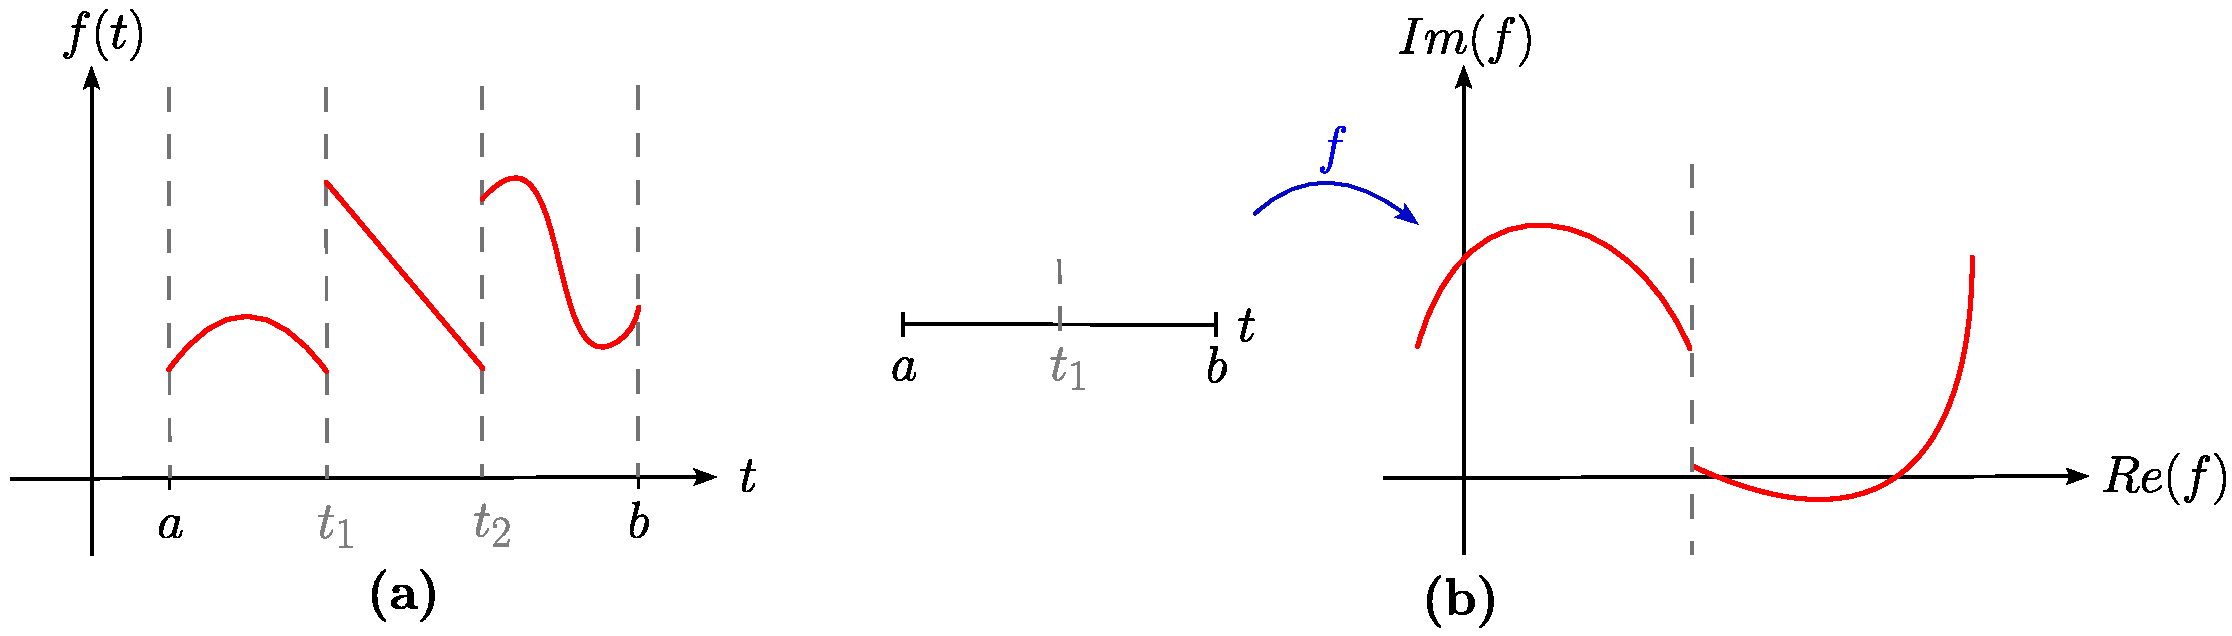
\includegraphics[scale=0.45]{Figuras/FuncionSC.pdf}
    \caption{En (a) una función de la forma $f: [a,b] \rightarrow \mathbb{R}$ y en (b) una función de la forma $f: [a,b] \rightarrow \mathbb{C}$, ambas seccionalmente continuas.}
    \label{fig:FunciónSC}
\end{figure}

Podemos afirmar que los conjuntos $\mathcal{C}_0 [a,b]$ y $\mathcal{C}[a,b]$ forman espacios vectoriales sobre el cuerpo de los complejos. Además, $\mathcal{C}_0 [a,b] \subset \mathcal{C} [a,b].$

\begin{defi}
Consideremos dos funciones $f,g \in \mathcal{C}[a,b]$. Definimos su \textbf{producto escalar} como
$$\boxed{\langle f , g \rangle = \int_a^b f(t) g^*(t) \,dt }$$
\end{defi}

\begin{propo}[Propiedades del producto escalar] \label{ProductoEscalar}
 Sean $f,g,h \in \mathcal{C}[a,b]$ y  $\lambda \in \mathbb{C}$.
 
 \begin{itemize}
     \item $\langle f , g \rangle = \langle g, f \rangle^*$
     \item $\langle f , g + h \rangle = \langle f , g \rangle + \langle f , h \rangle$
     \item $\langle f + g , h \rangle = \langle f , h \rangle + \langle g , h \rangle$
     \item $\langle \lambda f , g \rangle = \lambda \langle f , g \rangle$
     \item $\langle  f , \lambda g \rangle = \lambda^*\langle f , g \rangle$
     \item Si $f \not\equiv 0$, entonces $\langle f , f \rangle > 0$
 \end{itemize}
\end{propo}

\textbf{Observación:} Con respecto a la última propiedad, se tiene que 
$$\langle f , f \rangle = \int_a^b |f(t)|^2 \,dt = 0 ~\mbox{NO IMPLICA}~ f = 0.$$

Por esto se define la relación de equivalencia \footnote{$m(E) = 0$ denota que $E$ es un conjunto de medida cero.}
$$f = g ~ c.t.p ~\Leftrightarrow~ f(t) = g(t), \forall t \in [a,b]-E, \mbox{con}~ m(E) = 0.$$

Esta relación se expresa diciendo que $f = g $ casi en todas partes.

\textbf{Notación:} $f \equiv g ~\Leftrightarrow~ f = g ~c.t.p$

Esencialmente una relación de equivalencia es una relación de igualdad, bajo la cual dos funciones equivalentes se consideran ``iguales". Así, toda función $f = 0 ~c.t.p$, o simplemente $f\equiv 0$, se considera como la función nula.

\begin{defi}
Un espacio vectorial complejo dotado de un producto escalar con las propiedades de la proposición \ref{ProductoEscalar}, se conoce como \textbf{espacio pre-Hilbert}.
\end{defi} 

\begin{defi}
Sea $f \in \mathcal{C}[a,b]$. Definimos su \textbf{norma} como
$$\norm{f} = \sqrt{\langle f,f \rangle} \in \mathbb{R}.$$
\end{defi}

\begin{propo}
Sean $f,g \in \mathcal{C}[a,b]$ y $\lambda \in \mathbb{C}$.

\begin{itemize}
    \item $\norm{f} \geq 0$
    \item $\norm{\lambda f} = |\lambda| \norm{f}$
    \item $|\langle f| g \rangle | \leq \norm{f} \cdot \norm{g}$ (Desigualdad de Cauchy-Schwarz)
    \item $\norm{f \pm g} \leq \norm{f} + \norm{g}$ (Desigualdad triangular)
    \item Si $f \not\equiv 0$, entonces $\norm{f} > 0$.
\end{itemize}
\end{propo}

\begin{demo}
Demostraremos solo la desigualdad de Cauchy-Schwarz y la triangular.

\begin{itemize}
    \item \textbf{Desigualdad de Cauchy-Schwarz}:
    
    Sea $\lambda \in \mathbb{C}$ arbitrario,
\begin{align*}
0 \leq \norm{\lambda f + g}^2 = \langle \lambda f + g , \lambda f + g\rangle &= \langle \lambda f , \lambda f \rangle + \langle \lambda f , g \rangle + \langle g, \lambda f \rangle + \langle g , g \rangle \\
&= \lambda \lambda^* \norm{f}^2 + \lambda \langle f,g\rangle + \lambda^* \langle g,f\rangle + \norm{g}^2.
\end{align*}

Siendo $\lambda$ arbitrario, consideremos entonces
\begin{equation*}
    \lambda = - \frac{\langle g,f \rangle}{\norm{f}^2} ~\Rightarrow~ \lambda^* = - \frac{\langle f,g\rangle}{\norm{f}^2}, \quad \norm{f} \neq 0.
\end{equation*}

Luego, 
$$0 \leq \frac{|\langle f, g \rangle|^2}{\norm{f}^4} \norm{f}^2 - 2 \frac{|\langle f,g \rangle|^2}{\norm{f}^2} + \norm{g}^2 = -\frac{|\langle f,g \rangle|^2}{\norm{f}^2} + \norm{g}^2. $$

Lo que implica 
$$|\langle f,g \rangle|^2 \leq \norm{f}^2 \cdot \norm{g}^2 ~\Rightarrow~ \boxed{|\langle f , g \rangle| \leq \norm{f} \cdot \norm{g}}$$

Si suponemos que $\norm{f} = 0$, $f \equiv 0$ y la desigualdad se demuestra trivialmente.

 \item \textbf{Desigualdad triangular}: De la definición de norma
 \begin{align*}
     \norm{f\pm g}^2 = \langle  f \pm g , f \pm g \rangle &= \langle f \pm g , f \rangle \pm \langle f \pm g , g\rangle \\
     &= \langle f,f \rangle \pm \langle f , g \rangle^* \pm \langle f,g \rangle +  \langle g,g \rangle \\
     &= \norm{f}^2 \pm 2 Re(\langle f,g \rangle) + \norm{g}^2.
 \end{align*}
 
 Como $\pm Re(z) \leq |z|$ para todo $z \in \mathbb{C}$, obtenemos que 
 $$\norm{f\pm g}^2 \leq \norm{f}^2+ 2 |\langle f,g \rangle| + \norm{g}^2.$$
 
 Por la desigualdad de  Cauchy-Shwarz:
 $$\norm{f\pm g}^2 \leq \norm{f}^2 + 2 \norm{f} \cdot \norm{g} + \norm{g}^2 = (\norm{f} + \norm{g})^2 ~\Rightarrow~ \boxed{\norm{f \pm g} \leq \norm{f} + \norm{g}}$$
\end{itemize}


\end{demo}

\section{Sucesiones y series de funciones}

\begin{defi}[Sucesión de funciones]
Sea $\{f_n\}_{n \in \mathbb{N}}$ una sucesión de funciones 
$$f_n: D \subseteq \mathbb{R} \longrightarrow \mathbb{C}.$$

y considere $f: D \subseteq \mathbb{R} \longrightarrow \mathbb{C}$.

\begin{enumerate}
    \item Diremos que $\{f_n\}_{n \in \mathbb{N}}$ \textbf{converge puntualmente} a $f$ si dado $t \in D$ se tiene que la sucesión de números complejos $\{f_n(t)\}_{n \in \mathbb{N}}$ converge a $f(t)$ donde $f$ se llama la \textbf{función límite} de $\{f_n\}_{n \in \mathbb{N}}$, matemáticamente:
    $$(\forall t \in D)(\forall \varepsilon > 0)(\exists N(t,\varepsilon) \in \mathbb{N})(n \geq N ~\Rightarrow~ |f_n(t) - f(t)| < \varepsilon).$$
    
    \textbf{Notación:} $\lim\limits_{n \to + \infty} f_n(t) = f(t)$.
    
    \item  Diremos que $\{f_n\}_{n \in \mathbb{N}}$ \textbf{converge uniformemente} a $f$ si 
     $$(\forall \varepsilon > 0)(\exists N(\varepsilon) \in \mathbb{N})(n \geq N ~\wedge~ \forall t \in D ~\Rightarrow~ |f_n(t) - f(t)| < \varepsilon).$$
     
     \textbf{Notación:} $\lim\limits_{n \to + \infty} f_n(t) = f(t) ~[uniforme]$.
\end{enumerate}

\end{defi}

\textbf{Observación:} Es fácil de ver que si $\{f_n\}_{n\in \mathbb{N}}$ converge uniformemente a $f$, entonces $\{f_n\}_{n\in \mathbb{N}}$ converge puntualmente a $f$.

\begin{defi}[Serie de funciones]
Sea $\{f_n\}_{n \in \mathbb{N}}$ una sucesión de funciones
$$f_n: D \subseteq \mathbb{R} \longrightarrow \mathbb{C}.$$

Sea $F_n = \sum\limits_{k=1}^n f_k$. Se llama \textbf{serie de funciones} a la sucesión de sumas parciales $\{F_n\}_{n\in\mathbb{N}}$ y se denota por $\sum\limits_{n=1}^{\infty} f_n$.

\begin{enumerate}
    \item La serie $\sum\limits_{n=1}^{\infty} f_n$ converge (puntualmente) a $F$ si y solamente si $\{F_n\}_{n \in \mathbb{N}}$ converge puntualmente a $F$ sobre $D$.
    
    \textbf{Notación:} 
    $$\sum_{n=1}^{\infty} f_n = F = \lim_{n\to + \infty} \sum_{k=1}^n f_k.$$
    
    \item La serie $\sum\limits_{n=1}^{\infty} f_n$ converge uniformemente a $F$  sobre $D$ si y solamente si $\{F_n\}_{n \in \mathbb{N}}$ converge uniformemente a $F$ sobre $D$.
    
    \textbf{Notación:} 
    $$\sum_{n=1}^{\infty} f_n = F ~[uniforme].$$
    
    \item La serie $\sum\limits_{n=1}^{\infty} f_n$ converge absolutamente a $F$  sobre $D$ si y solamente si la serie $\sum\limits_{n=1}^{\infty} |f_n|$ converge puntualmente a $F$ sobre $D$.
    
\end{enumerate}
\end{defi}

\begin{defi}
La \textbf{distancia} entre dos funciones $f,g \in \mathcal{C}[a,b]$ se define por 
$$\boxed{\norm{f-g} = \sqrt{\int_a^b [f(t)-g(t)][f(t)-g(t)]^* dt}}$$
\end{defi}

A partir de la definición y las propiedades de la norma, se tiene que
$$\norm{f-g} = 0 ~\Leftrightarrow~ f \equiv g.$$

\begin{defi}
Un \textbf{espacio métrico} es un conjunto $X$ provisto de una \textbf{distancia} (o \textbf{métrica}) $d: X \times X \rightarrow \mathbb{R}$ que verifica:

\begin{enumerate}
    \item[(i)] $\forall x,y \in X: d(x,y) = 0 \Leftrightarrow x = y$.
    
    \item[(ii)] $\forall x,y \in X: d(x,y) = d(y,x)$.
    
    \item[(iii)] $\forall x,y,z \in X: d(x,y) \leq d(x,z) + d(z,y)$. (Desigualdad triangular)
\end{enumerate}
\end{defi}

\textbf{Observación:} Note que de las condiciones para una métrica, se desprende la no negatividad de la función $d$. En efecto, para todo $x,y \in X$, se tiene que
$$d(x,x) = 0 \leq d(x,y) + d(y,x) = d(x,y) + d(x,y) = 2  d(x,y) \Rightarrow d(x,y) \geq 0.$$

El par $(\mathcal{C}[a,b], \norm{\cdot})$ es un espacio métrico y como tal se introducen los conceptos de convergencia de sucesiones y series en el sentido de la distancia dada en este espacio. La convergencia en esta métrica se llama \textbf{convergencia en media} o \textbf{convergencia cuadrática}.

\begin{defi}
Sea $\{f_n\}_{n\in \mathbb{N}}$ una sucesión de elementos de $\mathcal{C}[a,b]$. Se dice que $\{f_n\}_{n\in \mathbb{N}}$ \textbf{converge en media} a $f \in \mathcal{C}[a,b]$ si 
\begin{equation*}
    \lim_{n \to + \infty} \norm{f_n - f} = 0.
\end{equation*}

Se escribe, $\lim\limits_{n \to + \infty} f_n = f ~[en ~media]$ en $[a,b]$.
\end{defi}

\textbf{Observación:}
\begin{shaded}
$$ \lim_{n \to + \infty} \norm{f_n - f} = 0  ~\Leftrightarrow~ \lim_{n \to + \infty} \int_a^b |f_n(t) - f(t)|^2 dt = 0.$$    
\end{shaded}

\begin{propo}
Considere $f,f_n \in \mathcal{C}[a,b]$, $n\in \mathbb{N}$. Si $\{f_n\}_{n \in \mathbb{N}}$ converge uniformemente a $f$, entonces $\{f_n\}_{n \in \mathbb{N}}$ converge en media a $f$.
\end{propo}

\begin{demo}
Por hipótesis tenemos que dado $\varepsilon > 0$, existe $N = N(\varepsilon) \in \mathbb{N}$ tal que
\begin{align*}
    n \geq N ~\wedge~ \forall t \in [a,b] &\Rightarrow |f_n(t) - f(t)| < \sqrt{\frac{\varepsilon}{b-a}} \\
    &\Rightarrow |f_n(t) - f(t)|^2 < \frac{\varepsilon}{b-a} \\
    &\Rightarrow \int_a^b |f_n(x) - f(x)|^2 \,dt < \varepsilon. \qquad \mbox{(Propiedad de Monotonía)}
\end{align*}

Por lo tanto, 
$$\forall\varepsilon > 0, \exists N \in \mathbb{N}: ~ n \geq N ~\Rightarrow~ \int_a^b |f_n(t) - f(t)|^2 \,dt < \varepsilon,$$

lo que muestra que $\{f_n\}_{n \in \mathbb{N}}$ converge en media a $f$

\end{demo}

\textbf{Observación:} No hay relación entre la convergencia en media y la convergencia puntual.

\begin{ejemplo}
Sea la sucesión de polinomios definidos por $p_n(x) = x^n, n \in \mathbb{N}$ para $x \in [-1,1]$.

\begin{figure}[H]
    \centering
    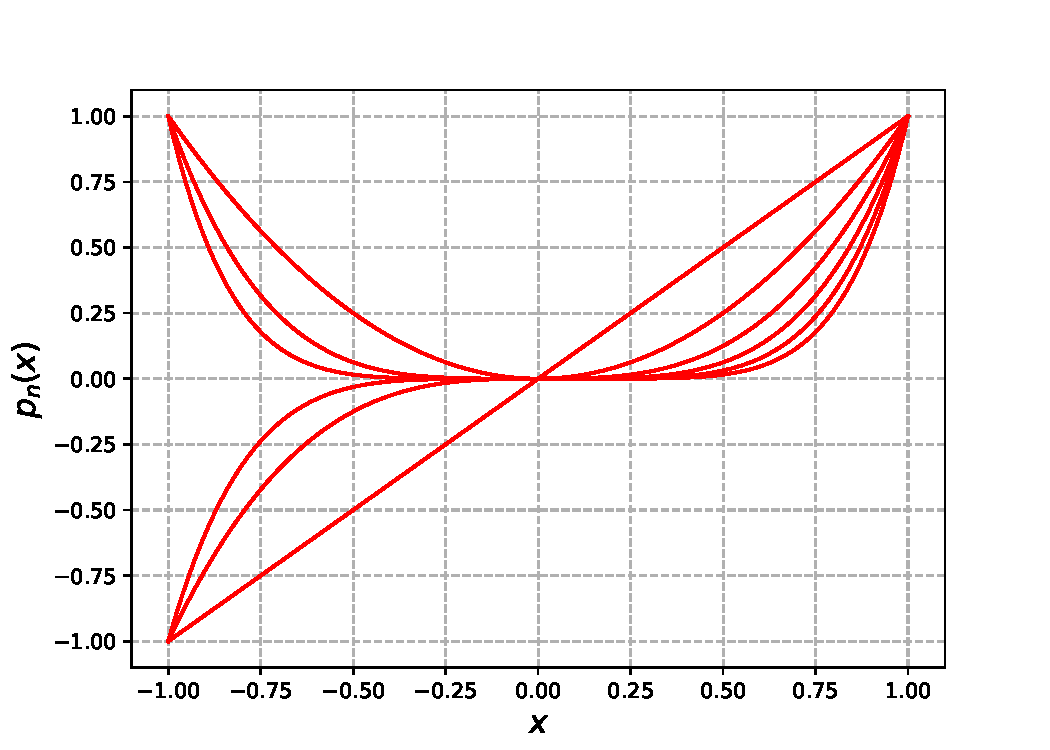
\includegraphics[scale = 0.57]{Figuras/SucesionPolinomios.pdf}
    \caption{Sucesión de polinomios $p_n(x) = x^n, x \in [-1,1]$ para $n = 1, \dots, 6$.}
\end{figure}

Ésta converge en media a $f \equiv 0$. En efecto, 
\begin{align*}
\lim_{n \to + \infty} \int_{-1}^1 |x^n - 0|^2 dx  = \lim_{n \to + \infty }  \int_{-1}^1 x^{2n} \,dx &= \lim_{n \to + \infty} \left. \frac{x^{2n+1}}{2n+1} \right|_{-1}^1 \\
&=  \lim_{n \to + \infty} \frac{2}{2n+1} = 0.
\end{align*}

Sin embargo, no converge puntualmente a $f$ sobre $[-1,1]$, pues 
$$\lim_{n \to + \infty} x^n = \left\{ \begin{array}{cl}
   0 ,& \mbox{si}~ -1 < x < 1 \\
   1  ,&  \mbox{si}~ x = 1 \\
   \mbox{diverge},&  \mbox{si}~ x = -1
\end{array}  \right. .$$

Luego, tampoco uniformemente a $f \equiv 0$ sobre $[-1,1]$.
\end{ejemplo}

\begin{defi}
Considere $f, f_n \in \mathcal{C}[a,b], n \in \mathbb{N}$ y $F_n = \sum\limits_{k=1}^n f_k$. Diremos que la serie $\sum\limits_{n=1}^{\infty} f_n$ \textbf{converge en media} a $f$ si la sucesión de sumas parciales $\{F_n\}_{n\in \mathbb{N}}$ converge en media a $f$. 
\\

\textbf{Notación:} 
$$\sum_{n=1}^{\infty} f_n(t) \sim f(t), \quad t \in [a,b]$$

o 
$$\sum_{n=1}^{\infty} f_n(t) = f(t) ~ [en ~media], \quad t \in [a,b].$$
\end{defi}

\textbf{Observación:}  
\begin{shaded}
$$\sum_{n=1}^{\infty} f_n(t) \sim f(t), \quad t \in [a,b] ~\Leftrightarrow~ \lim_{n \to + \infty} \int_a^b \left[ \sum_{k=1}^n f_k(t) - f(t)\right]^2 \, dt = 0.$$ 
\end{shaded}

\begin{defi}
Una sucesión $\{f_n\}_{n \in \mathbb{N}}$ en $\mathcal{C}[a,b]$ se dice \textbf{sucesión de Cauchy} si dado $\varepsilon > 0$, existe un $N \in \mathbb{N}$ tal que 
$$\forall n,m \geq N ~\Rightarrow~ \norm{f_n-f_m} < \varepsilon.$$
\end{defi}

La definición anterior se puede generalizar a espacios de funciones sin norma, pero con una métrica definida.

Es inmediato verificar que $\{f_n\}_{n \in \mathbb{N}}$ converge a una función $f$ en media, entonces es de Cauchy, pues 
$$\norm{f_n - f_m} \leq \norm{f_n - f} + \norm{f_m - f},$$

y ambos términos en el lado derecho se pueden acotar por un $\varepsilon > 0$ arbitrario para todo $n,m \geq N$. El inverso, sin embargo, es falso, como se puede apreciar en el siguiente ejemplo:

\begin{ejemplo}
Consideremos el conjunto de funciones reales 
 $\mathcal{C}_0[0,1]$, con el producto escalar definido como 
$$\langle f,g\rangle = \int_0^1 f(x) g(x) \,dx.$$

Sea  
\begin{equation*}
    f_n(x) = \left\{ \begin{array}{cl}
       1,  & \mbox{si} ~ 0 \leq x \leq \frac{1}{2}\\
    1 - \left(x - \frac{1}{2} \right)n,     & \mbox{si}  ~ \frac{1}{2} < x < \frac{1}{2} + \frac{1}{n} \\
    0, & \mbox{si} ~ \frac{1}{2} + \frac{1}{n} \leq x \leq 1
    \end{array} \right., n \geq 2.
\end{equation*}

\begin{figure}[H]
    \centering
    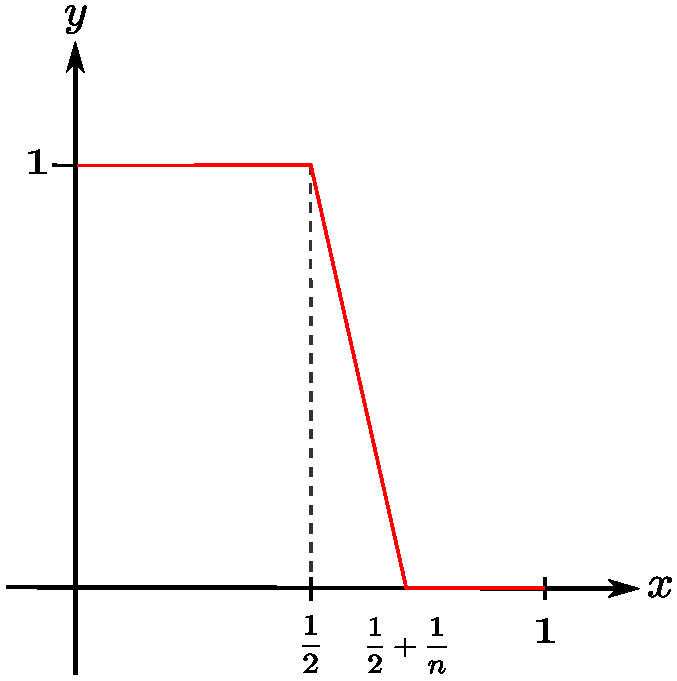
\includegraphics[scale = 0.5]{Figuras/EjemploCauchy.pdf}
    \caption{Ejemplo de sucesión de Cauchy que no converge en media a $C_0[0,1]$.}
\end{figure}

Para $m \geq n$, 
\begin{align*}
    \norm{f_n - f_m}^2 = \int_0^1 |f_n(x) - f_m(x)|^2 \,dx &= \int_0^{\frac{1}{2}} [1-1] \,dx + \int_{\frac{1}{2}}^{\frac{1}{2} + \frac{1}{n}} |f_n(x) - f_m(x)|^2 \,dx + \int_{\frac{1}{2} + \frac{1}{n}}^1 0 \, dx \\
    &=  \int_{\frac{1}{2}}^{\frac{1}{2} + \frac{1}{n}} |f_n(x) - f_m(x)|^2 \,dx.
\end{align*}

Ahora, para todo $x \in \left[\frac{1}{2}, \frac{1}{2}  + \frac{1}{n} \right]$, tenemos

$$|f_n(x) - f_m(x)| \leq |f_n(x)| + |f_m(x)| \leq 1 + 1 = 2. $$

Luego, 
\begin{equation*}
   \norm{f_n - f_m}^2  = \int_{\frac{1}{2}}^{\frac{1}{2} + \frac{1}{n}} |f_n(x) - f_m(x)|^2 \,dx \leq \int_{\frac{1}{2}}^{\frac{1}{2} + \frac{1}{n}} 4 \,dx = \frac{4}{n} ~\Rightarrow~ \norm{f_n - f_m} \leq \frac{2}{\sqrt{n}}.
\end{equation*}

Para $m < n$, es fácil de ver que 
$$\norm{f_n - f_m} \leq \frac{2}{\sqrt{m}}.$$

Así, dado $\varepsilon > 0$, por propiedad arquimediana, existe $N \in \mathbb{N}$ tal que 
$$N > \frac{4}{\varepsilon^2} $$

que verifica 
$$\forall m,n \geq N ~\Rightarrow~   \norm{f_n - f_m} < \varepsilon$$

de modo que es una sucesión de Cauchy. Sin embargo, $\{f_n\}$ converge en media a una función discontinua en $x = \frac{1}{2}$ (pruébelo!), y por lo tanto no converge en $\mathcal{C}_0[0,1]$.
\end{ejemplo}

\begin{defi}
Un espacio normado es llamado \textbf{completo} si toda sucesión de Cauchy es convergente. A un espacio normado completo se le llama \textbf{espacio de Banach}. A un espacio pre-Hilbert que es completo se le llama \textbf{espacio de Hilbert}
\end{defi}

\begin{defi}
El conjunto de funciones $\{\varphi_n(t)\}_{n=0, \pm 1, \pm 2, \dots}$ se dice \textbf{ortogonal} si 
$$\langle \varphi_n , \varphi_m \rangle = 0, \quad \mbox{para} ~ n \neq m.$$

Si además, $\norm{\varphi_n} = 1$ para cada $n \in \mathbb{Z}$, se dice que es un conjunto \textbf{ortonormal}, entonces podemos escribir 
$$\langle \varphi_n , \varphi_m \rangle = \delta_{nm}, \quad \forall n,m.$$
\end{defi}

\begin{ejemplo}
Como ejemplo de funciones ortonormales tenemos las $c_n(t) \in \mathcal{C}_0[-\pi,\pi]$ con $n = 0, \pm 1, \pm 2, \dots$ que se definen como
$$c_n(t) = \frac{1}{\sqrt{2\pi}} e^{i nt}.$$

En efecto, para $n \neq m$, se tiene que
\begin{align*}
    \langle c_n , c_m \rangle = \frac{1}{2\pi} \int_{-\pi}^{\pi} e^{i(n-m)t} \,dt &= \frac{1}{2\pi} \left[ -\frac{i}{n-m} e^{i(n-m) t}\right]_{-\pi}^{\pi} \\
    &= \frac{i}{2\pi(m-n)} [e^{i n\pi} + e^{-i m \pi} - e^{-in \pi} - e^{im \pi}] \\
    &= 0.
\end{align*}

Por otro lado, para $n = m$:
\begin{equation*}
  \langle c_n , c_n \rangle =\frac{1}{2\pi} \int_{-\pi}^{\pi} e^{i(n-n)t} \,dt = \frac{1}{2\pi} \int_{-\pi}^{\pi} 1 \,dt = 1.
\end{equation*}
$$\therefore  \langle c_n , c_m \rangle = \delta_{nm}.$$
\end{ejemplo}

\begin{ejemplo}
Pruebe que el conjunto de funciones 
$$\left\{ \frac{1}{\sqrt{2 \pi}}, \frac{\cos(nt)}{\sqrt{\pi}} ,  \frac{\sin(nt)}{\sqrt{\pi}} \right\}_{n=1}^{\infty}$$

es ortonormal en $\mathcal{C}[-\pi,\pi]$.
\\

\textbf{Solución}: Probemos primero la normalización.
\begin{align*}
    \int_{-\pi}^{\pi} \left( \frac{1}{\sqrt{2\pi}} \right)^2 \,dt &= 1, \\
    \int_{-\pi}^{\pi} \frac{\cos^2(nt)}{\pi} \,dt &=  \frac{1}{\pi} \int_{-\pi}^{\pi} \frac{1}{2} + \frac{1}{2} \cos(2n t) \,dt = 1, \\
    \int_{-\pi}^{\pi} \frac{\sin^2(nt)}{\pi} \,dt &=  \frac{1}{\pi} \int_{-\pi}^{\pi} \frac{1}{2} - \frac{1}{2} \cos(2n t) \,dt = 1.
\end{align*}

Para la ortogonalidad, tengamos en cuenta las siguientes identidades trigonométricas:
\begin{align*}
    \sin \alpha \sin \beta &= \frac{1}{2} [\cos(\alpha - \beta) - \cos(\alpha + \beta)], \\
    \cos \alpha \cos \beta &= \frac{1}{2} [\cos(\alpha - \beta) + \cos(\alpha + \beta)], \\
    \sin \alpha \cos \beta &= \frac{1}{2} [\sin(\alpha + \beta) + \sin(\alpha - \beta)].
\end{align*}

Entonces, 
\begin{align*}
    \int_{-\pi}^{\pi} \frac{1}{\sqrt{2} \pi} \cos(nt) \,dt &=  \left. \frac{1}{\sqrt{2}\pi n} \sin(nt) \right|_{-\pi}^{\pi} = 0, \\
     \int_{-\pi}^{\pi} \frac{1}{\sqrt{2} \pi} \sin(nt) \,dt &=   \left. - \frac{1}{\sqrt{2}\pi n} \cos(nt) \right|_{-\pi}^{\pi} = 0,\\
      \int_{-\pi}^{\pi} \frac{1}{\pi} \cos(n t) \sin(m t)\,dt &=  \frac{1}{2 \pi} \int_{-\pi}^{\pi} \sin(m+n)t + \sin(m-n)t \ dt = 0; \quad n,m \in \mathbb{N}. 
\end{align*}

Para todo $n, m \in \mathbb{N}$, $m \neq n$, se tiene que 
\begin{align*}
    \int_{-\pi}^{\pi} \frac{1}{\pi} \cos(n t) \cos(mt) \,dt &= \frac{1}{2\pi} \int_{-\pi}^{\pi} \cos(n-m)t + \cos(n+m) t\,dt \\
    &= \frac{1}{2\pi} \left[ \frac{1}{n-m} \sin(n-m)t + \frac{1}{n+m} \sin(n+m)t \right]_{-\pi}^{\pi} = 0. \\
     \int_{-\pi}^{\pi} \frac{1}{\pi} \sin(n t) \sin(mt) \,dt &=\frac{1}{2\pi} \int_{-\pi}^{\pi} \cos(n-m)t - \cos(n+m) t\,dt  \\
    &= \frac{1}{2\pi} \left[ \frac{1}{n-m} \sin(n-m)t - \frac{1}{n+m} \sin(n+m)t \right]_{-\pi}^{\pi} = 0.
\end{align*}

Por lo tanto, 
$$\left\{ \frac{1}{\sqrt{2 \pi}}, \frac{\cos(nt)}{\sqrt{\pi}} ,  \frac{\sin(nt)}{\sqrt{\pi}} \right\}_{n=1}^{\infty}$$

es ortonormal en $\mathcal{C}[-\pi,\pi]$.
\end{ejemplo}

\begin{defi}
Sea $S = \{\varphi_n(t)\}_{n=0, \pm 1, \pm 2, \dots}$. Se dice que $S$ es \textbf{linealmente independiente} (l.i.) si todo subconjunto finito de $S$ también lo es.
\end{defi}

\begin{propo} \label{LIortogonal}
Todo conjunto ortogonal en $\mathcal{C}[a,b]$ que no contenga al vector nulo es linealmente independiente.
\end{propo}

\begin{demo}
Sea $S = \{\varphi_n(t)\}_{n=0, \pm 1, \pm 2, \dots}$ ortogonal tal que $\varphi_n \not\equiv 0, \forall n$. Consideremos el subconjunto finito de $S$, $S' = \{\varphi_{i_1}, \dots, \varphi_{i_n}\}$ y además la combinación lineal
$$\alpha_1 \varphi_{i_1} + \alpha_2 \varphi_{i_2} + \cdots + \alpha_n \varphi_{i_n} \equiv 0.$$

Entonces, para un cierto $\varphi_{i_m}$, se tiene que
$$\langle \alpha_1 \varphi_{i_1} + \alpha_2 \varphi_{i_2} + \cdots + \alpha_n \varphi_{i_n},\varphi_{i_m} \rangle = \alpha_m \underbrace{\norm{\varphi_{i_m}}^2}_{\neq 0} = 0.$$

Por lo tanto, 
$$\alpha_m = 0, \quad m = 1, 2, \dots, n$$

probando así que $S'$ es linealmente independiente y en consecuencia $S$ es l.i.
\end{demo}

\section{Proceso de ortonormalización de Gram-Schmidt}

Sea $\{v_n\}_{n = 1,2, \dots}$ un conjunto linealmente independiente de funciones en $\mathcal{C}[a,b]$. Para construir un conjunto ortonormal debemos seguir los siguientes pasos:

\begin{enumerate}
    \item Construimos 
    $$\varphi_1 = \frac{v_1}{\norm{v_1}}$$ 
    
    tal que $\langle \varphi_1 , \varphi_1 \rangle = 1$. 
    
    \item Consideramos
    $$\overline{\varphi}_2 = v_2 - \langle v_2, \varphi_1   \rangle \varphi_1.$$
    
    Entonces, 
    $$\langle \overline{\varphi}_2, \varphi_1 \rangle = \langle v_2, \varphi_1 \rangle - \langle  v_2, \varphi_1  \rangle \langle \varphi_1, \varphi_1 \rangle = \langle v_2, \varphi_1 \rangle -  \langle  v_2, \varphi_1 \rangle  = 0.$$
    
    Normalizando, 
    $$\varphi_2 = \frac{\overline{\varphi}_2}{\norm{\overline{\varphi}_2}}.$$
    
    \item En general para un cierto $n \geq 2$, consideremos 
 $$\overline{\varphi}_n = v_n - \sum_{j=1}^{n-1} \langle  v_n, \varphi_j \rangle \varphi_j.$$
    
Entonces, para $1 \leq  i \leq n-1$, tenemos que
\begin{align*}
    \langle \Bar{\varphi}_n , \varphi_i \rangle &= \langle v_n , \varphi_i \rangle - \sum_{j=1}^{n-1} \langle v_n , \varphi_j \rangle \langle \varphi_j , \varphi_i\rangle \\
    &= \langle v_n, \varphi_i \rangle - \sum_{j=1}^{n-1} \langle v_n , \varphi_j \rangle \delta_{ji} \\
    &= \langle v_n , \varphi_i \rangle -  \langle v_n, \varphi_i \rangle = 0.
\end{align*}
    
Finalmente, normalizando    
$$\varphi_n = \frac{\overline{\varphi}_n}{\norm{\overline{\varphi}_n}}.$$
\end{enumerate}

El conjunto de funciones $\{\varphi_n\}_{n = 1,2, \dots}$ construido de la manera anterior es un conjunto ortonormal.

Geométricamente, el método se encuentra ilustrado en la figura \ref{fig:Gram-Schmidt}, donde se ha considerado las funciones como vectores y solo el proceso de ortogonalización.

\begin{figure}[H]
    \centering
    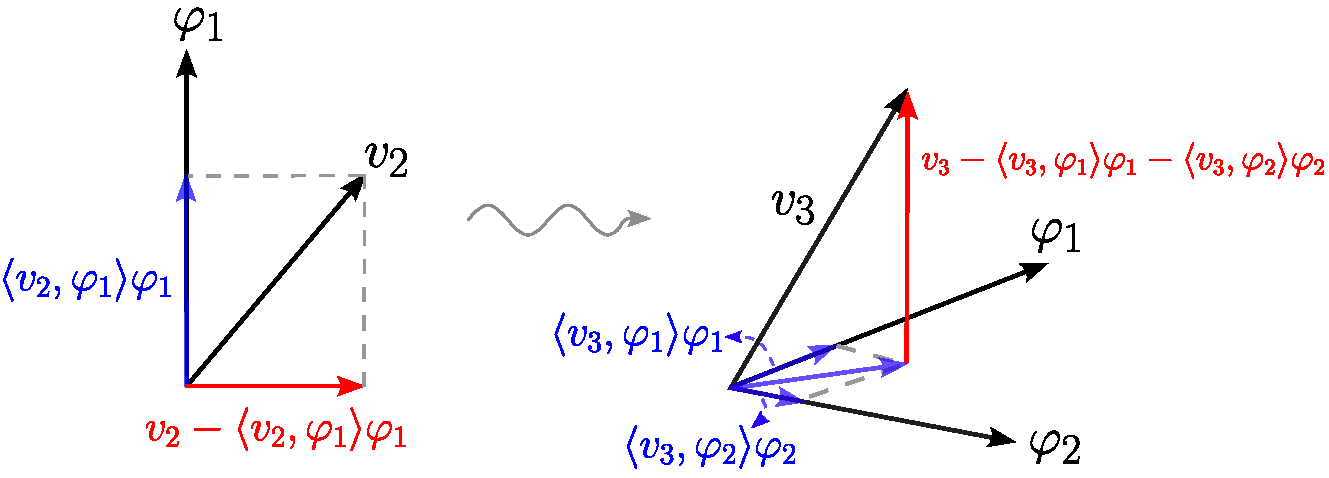
\includegraphics[scale = 0.7]{Figuras/Gram-Schmidt.pdf}
    \caption{Proceso de ortogonalización (sin la normalización) de Gram-Schmidt para tres funciones $\{v_1,v_2,v_3\}$.}
    \label{fig:Gram-Schmidt}
\end{figure}

\newpage
\section{Coeficientes de Fourier}

Ahora, definiremos un espacio de funciones más general que $\mathcal{C}[a,b]$, las funciones cuadrado integrables. \footnote{La condición de cuadrado integrable es usada, por ejemplo, en Mecánica Cuántica, pues constituye la base para que las funciones de onda describan el comportamiento de los sistemas físicos, consecuencia de la interpretación de Copenhague (probabilística) de la mecánica cuántica.}

\begin{defi}
    Definimos $\mathcal{L}^2[a,b]$ como el espacio de funciones $f:[a,b] \rightarrow \mathbb{C}$, tales que 
    $$\int_a^b |f(t)|^2 \,dt < \infty.$$
\end{defi}

\begin{teorema}
El espacio $\mathcal{L}^2[a,b]$ es un espacio vectorial con producto interno 
$$\langle f,g \rangle = \int_a^b f(t) g^* (t) \,dt$$

y norma
$$\norm{f} = \left( \int_a^b |f(t)|^2 \,dt \right)^{1/2}.$$
\end{teorema}

La demostración requiere verificar las propiedades del producto interno (escalar) dadas por \ref{ProductoEscalar}, la cual está fuera de los alcances de los contenidos de este apunte. \footnote{Para más información puede consultar bibliografía relacionada a la integral de Lebesgue.} 

\textbf{Observación:} Las funciones seccionalmente continuas son funciones cuadrado integrables.
\\

Sea $\{\varphi_{\nu}(t)\}_{\nu \in \mathbb{N}}$ un conjunto ortonormal de funciones tales que $\varphi_{\nu} \in \mathcal{C}[a,b]$ para todo $\nu \in \mathbb{N}$. Sea $f(t)$ una función cuadrado integrable en $[a,b]$. Deseamos aproximar $f(t)$ por una suma finita 
$$S_n(t) = \sum_{\nu = 1}^n C_{\nu} \varphi_{\nu}(t),$$

de manera que $\norm{f - S_n}$ sea mínimo. Es decir, el objetivo es encontrar los coeficientes $C_{\nu}$ de modo que el \textbf{error cuadrático medio}
$$M_n(f) = \norm{f-S_n}^2 = \int_a^b \left| f(t) - \sum_{\nu = 1}^n C_{\nu} \varphi_{\nu}(t) \right|^2 \,dt,$$

sea mínimo. Evaluemos el error cuadrático medio
\begin{align}
    M_n(f) &= \int_a^b \left( f(t) - \sum_{\nu = 1}^n C_{\nu} \varphi_{\nu}(t)  \right) \left( f(t) - \sum_{\nu = 1}^n C_{\nu} \varphi_{\nu}(t) \right)^* \,dt \nonumber \\
    &= \int_a^b |f(t)|^2 \, dt  + \sum_{\nu = 1}^n |C_{\nu}|^2 \int_a^b |\varphi_{\nu}(t)|^2 \,dt - \sum_{\nu = 1}^n C_{\nu}^* \int_a^b f(t) \varphi_{\nu}^*(t) \,dt \nonumber \\
    & \quad - \sum_{\nu = 1}^n C_{\nu} \int_a^b f^*(t) \varphi_{\nu}(t) \,dt  \nonumber \\
    &= \norm{f}^2 + \sum_{\nu = 1}^n |C_{\nu}|^2 - \sum_{\nu = 1}^n C_{\nu}^* \langle f, \varphi_{\nu} \rangle - \sum_{\nu = 1}^n C_{\nu} \langle f, \varphi_{\nu} \rangle^* + \sum_{\nu = 1}^n |\langle f, \varphi_{\nu} \rangle|^2 - \sum_{\nu = 1}^n |\langle f, \varphi_{\nu} \rangle|^2\nonumber  \\
    &= \norm{f}^2  - \sum_{\nu = 1}^n |\langle f, \varphi_{\nu} \rangle|^2 + \sum_{\nu = 1}^n |C_{\nu} - \langle f , \varphi_{\nu} \rangle|^2 \geq 0, \label{ErrorMedio}
\end{align}

ya que la norma es mayor o igual a cero siempre. Claramente el mínimo se obtiene cuando $C_{\nu} = \langle f, \varphi_{\nu} \rangle$. 

De lo anterior se desprende: 
\begin{shaded}
 \begin{equation}
 \sum_{\nu = 1}^n |C_{\nu}|^2 = \sum_{\nu = 1}^n |\langle f , \varphi_{\nu} \rangle|^2 \leq \norm{f}^2  \qquad \mbox{\textbf{Desigualdad de Bessel}} \label{D.Bessel}.
\end{equation}
 
\end{shaded}

Como el número a la derecha de la desigualdad es independiente de $n$, la suma está acotada superiormente. Siendo todos sus términos no negativos, tenemos que
$$\sum_{\nu = 1}^{\infty} |C_{\nu}|^2 < \infty ~\Rightarrow~ \lim_{\nu \to + \infty} |C_{\nu}|^2 = 0 ~\Rightarrow ~ \lim_{\nu \to + \infty} \langle f , \varphi_{\nu} \rangle = 0.$$

Luego,
\begin{equation*}
 \sum_{\nu = 1}^{\infty} |C_{\nu}|^2 = \sum_{\nu = 1}^{\infty} |\langle f , \varphi_{\nu} \rangle|^2 \leq \norm{f}^2    .
\end{equation*}

\begin{defi}
Los coeficientes $\langle f , \varphi_{\nu}\rangle$ son llamados los \textbf{coeficientes de Fourier} de $f$  respecto al sistema ortonormal $\{\varphi_{\nu}\}_{\nu = 1,2, \dots}$. La serie $\sum\limits_{\nu = 1}^{\infty} C_{\nu} \varphi_{\nu}(t)$ se llama \textbf{serie generalizada de Fourier} de $f$ relativa al sistema ortonormal $\{\varphi_{\nu}\}_{\nu = 1,2, \dots}$.

\end{defi}

\begin{defi}
Si un conjunto de funciones $\{\varphi_{\nu}\}$ en cierto espacio permite aproximar en la norma (en media), con sus combinaciones lineales, cualquier función $f$ del espacio tan bien como se quiera, es decir,
$$\left\Vert f - \sum_{\nu} C_{\nu} \varphi_{\nu} \right\Vert< \varepsilon, \qquad \mbox{para $\varepsilon$ arbitrario},$$

se dice que es un \textbf{conjunto completo} respecto a este espacio.
\end{defi}

Sean $C_{\nu} = \langle f , \varphi_{\nu} \rangle$ los coeficientes de Fourier de $f$ respecto del conjunto ortonormal  $\{\varphi_{\nu}\}$, entonces la completitud de este conjunto se puede expresar por 
$$\lim_{n \to + \infty} \left\Vert f - \sum_{\nu =1}^{n} C_{\nu} \varphi_{\nu} \right\Vert = 0,$$

es decir, 
$$f \sim \sum_{\nu = 1}^{\infty} C_{\nu} \varphi_{\nu}.$$

Lo anterior NO implica que $f(t) = \sum\limits_{\nu = 1}^{\infty} C_{\nu} \varphi_{\nu}(t)$ en algún otro sentido (convergencia puntual o uniforme). Si
$$f \sim \sum_{\nu = 1}^{\infty} C_{\nu} \varphi_{\nu},$$

entonces de la relación \eqref{ErrorMedio}, tenemos 
\begin{equation*}
    \lim_{n \to + \infty} \left\Vert f - \sum_{\nu = 1}^n  C_{\nu} \varphi_{\nu} \right\Vert^2 = \lim_{n \to + \infty} \left\{ \Vert f \Vert^2 - \sum_{\nu = 1}^{n} |C_n|^2 \right\} = \norm{f}^2  - \sum_{\nu = 1}^{\infty} |C_n|^2 = 0.
\end{equation*}

Lo que implica que
\begin{shaded}
 \begin{equation}
    \norm{f}^2  = \sum_{\nu =1 }^{\infty} |C_{\nu}|^2 \qquad \mbox{\textbf{Igualdad de Parseval}}
\end{equation}   
\end{shaded}

\textbf{Observación:} El conjunto ortogonal completo $\{\varphi_{\nu}\}$ se le conoce también como \textbf{base ortogonal} del espacio de funciones en cuestión.

\begin{ejemplo}
El conjunto $\left\{ \frac{1}{\sqrt{2 \pi}} e^{i n t} \right\}_{n \in \mathbb{Z}}$ es ortonormal completo respecto a $[-\pi,\pi]$.
$$f(t) \sim \sum_{n = - \infty}^{\infty} C_n \frac{e^{int}}{\sqrt{2\pi}} ~\Rightarrow~ \int_{-\pi}^{\pi} |f|^2 \,dt = \sum_{n=- \infty}^{\infty} |C_n|^2 = \norm{f}^2 .$$
\end{ejemplo}


\begin{teorema}{}{} 
Si el conjunto ortonormal $\{\phi_{\nu}\}$ es completo respecto a $\mathcal{C}[a,b]$, entonces en $\mathcal{C}[a,b]$ la única función ortonormal a todo $\varphi_{\nu}$ es $f(t) \equiv 0$.
\end{teorema}

\begin{demo}
Sea $f$ una función ortonormal a todo $\varphi_{\nu}$, si $f(t_0) \neq 0$ para algún $t_0 \in [a,b]$, la función también es no nula en una vecindad en torno a $t_0$ (por continuidad), por lo tanto 
$$\int_a^b |f(t)|^2 \,dt = \norm{f}^2  > 0,$$

pero usando la igualdad de Parseval, tenemos para la norma de $f$ que
$$\norm{f}^2  = \sum_{\nu} |C_{\nu}|^2 = \sum_{\nu} |\langle f ,\varphi_{\nu} \rangle|^2 > 0,$$

es decir, $f$ no es ortogonal a todos los $\varphi_{\nu}$, lo cual es una contradicción. Luego, $f$ debe ser idénticamente nula.
\end{demo}

\begin{teorema}
Sea $\{S_n(t) \in \mathcal{C}_0[a,b]\}$; si existe $F(t)$ tal que la sucesión $S_n(t) = \sum\limits_{\nu = 1}^n C_{\nu} \varphi_{\nu}(t)$ converge uniformemente a $F(t)$, entonces $F(t)$ es continua, es decir, $F(t) \in \mathcal{C}_0[a,b]$.
\end{teorema}

\begin{demo}
Por convergencia uniforme, dado $\varepsilon > 0$, $\exists N \in \mathbb{N}$ tal que
$$n \geq N \wedge \forall t \in [a,b] ~\Rightarrow~ |S_n(t) - F(t)| < \frac{\varepsilon}{3}.$$

Además, por la continuidad de $S_n$ para todo $t_0 \in [a,b]$, existe $\delta(\varepsilon, N, t_0)$ tal que
$$\forall t \in [a,b]: ~ 0 < |t-t_0| < \delta ~\Rightarrow~ |S_N(t) - S_N(t_0)| < \frac{\varepsilon}{3}.$$

Por lo tanto, 
\begin{align*}
 \forall t \in [a,b]: ~ 0 < |t-t_0| < \delta &\Rightarrow |F(t) - F(t_0)|  \\
 &= |F(t) - S_n(t) + S_n(t) - S_n(t_0) + S_n(t_0) - f(t_0)| \\
 &\leq |F(t) - S_n(t)| + |S_n(t) - S_n(t_0)| + |S_n(t_0) - F(t_0)| \\
 &\leq \frac{\varepsilon}{3} + \frac{\varepsilon}{3} + \frac{\varepsilon}{3} = \varepsilon .
\end{align*}
\end{demo}

Este teorema nos asegura que una función discontinua no puede ser aproximada uniformemente por una familia de funciones continuas (por ejemplo, las funciones sinusoidales).

\begin{teorema}
Si dos funciones $f,g \in \mathcal{C}[a,b]$ tienen igual expansión en base completa (en el sentido de aproximación en la norma), entonces $f(t) = g(t)$.
\end{teorema}

\begin{demo}
Sea
$$S(t) = \sum_{\nu = 1}^{\infty} \langle f, \varphi_{\nu}\rangle \varphi_{\nu}(t)$$

la aproximación en la norma para $f$ y $g$. Luego, 
$$\Vert f-S \Vert = \Vert g-S \Vert = 0.$$

Así, 
\begin{equation*}
    \Vert f-g \Vert = \Vert f-S+S-g \Vert \leq \Vert f-S \Vert + \Vert S-g \Vert = 0 +0 = 0 ~\Rightarrow~ f = g.
\end{equation*}

\end{demo}

\section{Convergencia según Cesàro*}

Si consideramos la serie
$$\frac{1}{1-x} = \sum_{n=1}^{\infty} x^{n-1} = 1 + x + x^2 + x^3 + \cdots$$

ella converge para $|x|< 1$. A pesar de lo anterior evaluemos la función y su expansión en serie en $x = -1$:
$$\left. \frac{1}{1-x} \right|_{x= -1} \overset{?}{=} \frac{1}{2} = 1 - 1 + 1 -1 +1 -1 + \cdots$$

¿Será posible sumar la serie de modo que ésta sí converja al valor de la función en ese punto?

\begin{defi}
Sea $s_n$ la suma parcial $n$-ésima de la serie $\sum\limits_{n=1}^{\infty} a_n$ y sea $\{\sigma_n\}_{n\in \mathbb{N}}$ la sucesión de las medias aritméticas definidas por
$$\sigma_n = \frac{s_1 + \cdots + s_n}{n}, \quad n = 1, 2, \dots$$

La serie $\sum\limits_{n=1}^{\infty} a_n$ es \textbf{sumable de Cesàro} si $\{\sigma_n\}_{n\in \mathbb{N}}$ converge. Si $\lim\limits_{n \to + \infty} \sigma_n = S^*$, entonces $S^*$ se llama \textbf{suma de Cesàro} de $\sum\limits_{n=1}^{\infty} a_n$ y se escribe 
$$ \sum_{n=1}^{\infty} ^*   a_n = S^*.$$
\end{defi}

\begin{ejemplo}
Sea $a_n = x^{n-1}$ con $x \neq 1$. Entonces
$$s_n = \frac{1}{1-x} - \frac{x^n}{1-x} \qquad \mbox{(Demuéstrelo!!)}$$

y
\begin{align*}
 \sigma_n = \frac{1}{n} \sum_{k=1}^n \left\{\frac{1}{1-x} - \frac{x^k}{1-x} \right\} &= \frac{1}{1-x} - \frac{1}{n(1-x)} \sum_{k =1}^{n} x^k   \\
 &=\frac{1}{1-x} -  \frac{1}{n} \frac{x(1-x^n)}{(1-x)^2}.
\end{align*}

Por consiguiente, 
$$\sum_{n=1}^{\infty}^* x^{n-1} = \lim_{n \to +\infty} \left\{ \frac{1}{1-x} -  \frac{1}{n} \frac{x(1-x^n)}{(1-x)^2}\right\} = \frac{1}{1-x}; \quad |x| \leq 1, x \neq 1. $$

En particular,
$$\sum_{n=1}^{\infty}^* (-1)^{n-1} = \frac{1}{2}.$$

\end{ejemplo}

Note que la idea de la definición de sumabilidad de Cesàro es encontrar una forma de dar significado a series que en otro caso serían divergentes.
\\

\textbf{Observación}: La convergencia ordinaria necesita que el $\lim\limits_{n \to + \infty} \sum\limits_{k = 1}^n a_{k}$ exista. 

\hspace{2.45cm} La convergencia según Cesàro necesita que el $\lim\limits_{n \to + \infty} \frac{1}{n} \sum\limits_{k = 1}^n  \sum\limits_{l = 1}^{k} a_{l}$ exista.

\begin{teorema}
Si una serie es convergente con suma $S$, entonces es sumable de Cesàro con suma $S^* = S$.
\end{teorema}

Problemas similares a la serie discreta anterior ofrece calcular la integral, desde cero hasta infinito, de una función oscilante, que no decrece, del tipo $\int_0^{\infty} \sin(\omega x) \,dx$.

En el espíritu del caso discreto, proponemos la siguiente definición.

\begin{defi}
Definimos una \textbf{integral de Cesàro} de la siguiente manera:
\begin{equation}
    ^* \int_0^{\infty} f(t) \,dt = \lim_{y \to \infty } \frac{1}{y} \left\{ \int_0^y \int_0^x f(t) \,dt dx \right\}. \label{IntegralCesaro1}
\end{equation}

\end{defi}


Podemos encontrar una expresión alternativa para la integral de Cesàro integrando por partes la ecuación \eqref{IntegralCesaro1}:
\begin{align*}
    ^* \int_0^{\infty} f(t) \,dt &= \lim_{y \to \infty } \frac{1}{y} \left\{ \int_0^y \int_0^x f(t) \,dt dx \right\} \\
    &= \lim_{y \to \infty } \frac{1}{y} \left\{\left. x \int_0^x f(t)\,dt \right|_0^y - \int_0^y x f(x) \,dx \right\} \\
    &= \lim_{y \to \infty } \frac{1}{y} \left\{ y \int_0^y f(t) \,dt - \int_0^y xf(x) \,dx \right\}
\end{align*}
\begin{equation}
    \Rightarrow ~  \boxed{^* \int_0^{\infty} f(t) \,dt = \lim_{y \to \infty} \int_0^y \left( 1 - \frac{x}{y} \right) f(x) \,dx} \label{IntegralCesaro2}
 \end{equation}
 
 \begin{ejemplo}
Evalúe la integral de Cesàro de la función $f(x) = \sin(\omega x)$ con $\omega \neq 0$.
\\

\textbf{Solución:} Usando la ecuación \eqref{IntegralCesaro1}, obtenemos que
\begin{align*}
      ^* \int_0^{\infty} \sin(\omega t) \,dt &= \lim_{y \to \infty } \frac{1}{y} \left\{ \int_0^y \int_0^x \sin(\omega t) \,dt dx \right\} \\
      &= \lim_{y \to \infty } \frac{1}{y} \int_0^y \left[ \frac{1 - \cos(\omega x)}{\omega}\right] \, dx \\
      &= \lim_{y \to \infty} \left[ \frac{1}{\omega} - \frac{1}{\omega^2} \frac{\sin(\omega y)}{y}\right]
\end{align*}
\begin{equation}
    \Rightarrow ~  \boxed{^* \int_0^{\infty} \sin(\omega t) \,dt = \frac{1}{\omega}} \label{CesaroSeno}
 \end{equation}

 \end{ejemplo}
 
  \begin{ejemplo}
Evalúe la integral de Cesàro de la función $f(x) = \cos(\omega x)$ con $\omega \neq 0$.
\\

\textbf{Solución:} Usando la ecuación \eqref{IntegralCesaro1}, obtenemos que
\begin{align*}
      ^* \int_0^{\infty} \cos(\omega t) \,dt &= \lim_{y \to \infty } \frac{1}{y} \left\{ \int_0^y \int_0^x \cos(\omega t) \,dt dx \right\} \\
      &= \lim_{y \to \infty } \frac{1}{y} \int_0^y \frac{\sin(\omega x)}{\omega} \, dx \\
      &= \lim_{y \to \infty} \left[ \frac{1}{\omega^2 y} - \frac{\cos(\omega y)}{\omega^2 y} \right]
\end{align*}
\begin{equation}
    \Rightarrow ~  \boxed{^* \int_0^{\infty} \cos(\omega t) \,dt = 0 } \label{CesaroCoseno}
 \end{equation}

 \end{ejemplo}
\chapter{Análisis de Fourier}

\section{Periodicidad y paridad de funciones}

\subsection{Funciones periódicas}

\begin{defi}
Una función $f: \mathbb{R} \longrightarrow \mathbb{C} $ se dice que es \textbf{periódica de período $T$}, $T\neq 0$, si 
\begin{equation}
f(t) = f(t +T ), \quad \forall t.    \label{Periodica}
\end{equation}

La constante $T$ la tomaremos como la  menor constante positiva que satisface la igualdad \eqref{Periodica}.
\end{defi}

\textbf{Observación:} No es difícil de ver que se verifica:

\begin{enumerate}
    \item $$f(t) = f(t + nT), \quad n = 0, \pm 1, \pm 2, \dots$$
    
    \item Si $f(t)$ y $g(t)$ son funciones periódicas de período $T$, entonces la función
    $$h(t) = \alpha f(t) + \beta g(t); \quad \alpha, \beta \in \mathbb{C},$$
    
    tiene el mismo período $T$.
\end{enumerate}

\begin{ejemplo}
Encontrar el período de la función $f(t) = \cos \frac{t}{3} + \cos \frac{t}{4}$.
\\

\textbf{Solución:} Si la función $f(t)$ es periódica con período $T$, entonces, de \eqref{Periodica},
$$\cos \frac{1}{3}(t + T) + \cos \frac{1}{4}(t + T) = \cos \frac{t}{3} + \cos \frac{t}{4}.$$

Como $\cos(\theta + 2\pi n) = \cos \theta, n \in \mathbb{Z}$, obtenemos que 
$$\frac{1}{3} T = 2\pi n, \quad \frac{1}{4}T = 2\pi m; \quad n,m \in \mathbb{Z}.$$

Por consiguiente $T = 6\pi n = 8\pi m$; cuando $n = 4$ y $m=3$, se obtiene el mínimo valor de $T$. Así, $T = 24\pi$.
\end{ejemplo}

En general, si la función 
$$f(t) = \cos (\omega_1 t) + \cos (\omega_2 t)$$

es periódica de período $T$, entonces es posible encontrar dos enteros $n$ y $m$ tales que 
\begin{align}
    \omega_1 T &= 2\pi n,  \label{Periodica1}\\
     \omega_2 T &= 2\pi m. \label{Periodica2}
\end{align}

El cociente de \eqref{Periodica1} y \eqref{Periodica2} es
$$\frac{\omega_1}{\omega_2} = \frac{n}{m},$$

es decir, la relación $\omega_1/ \omega_2$ debe ser un número racional.

\begin{propo}
Sea $f: \mathbb{R} \longrightarrow \mathbb{C}$ una función periódica de período $T$. Sea $a \in \mathbb{R}$, entonces
$$ \int_{a-T/2}^{a + T/2} f(t) \,dt = \int_{- T/2}^{T/2} f(t) \,dt .$$
\end{propo}

\begin{demo}
Utilizando la propiedad de aditividad de la integral compleja:
\begin{equation*}
    \int_{a-T/2}^{a + T/2} f(t) \,dt = \int_{a - T/2}^{-T/2} f(t) \,dt + \int_{- T/2}^{a + T/2} f(t) \,dt.
\end{equation*}

Haciendo la sustitución  $t = t' - T ~\Rightarrow~ dt = dt'$ en la primera integral, obtenemos
\begin{align*}
   \int_{a - T/2}^{-T/2}f(t) \,dt + \int_{- T/2}^{a + T/2} f(t) \,dt   &= \int_{a + T/2}^{T/2} f(t'-T) \,dt' + \int_{- T/2}^{a + T/2} f(t) \,dt \\
   &= \int_{a + T/2}^{T/2} f(t'-T + T) \,dt' + \int_{- T/2}^{a + T/2} f(t) \,dt \\
   &= \int_{a + T/2}^{T/2} f(t') \,dt' + \int_{-T/2}^{a + T/2} f(t) \,dt \\
   &= \int_{-T/2}^{T/2} f(t) \,dt.
\end{align*}
\end{demo}

\begin{defi}
Sea $f: [a,b] \rightarrow \mathbb{R}$ seccionalmente continua, se llama \textbf{extensión periódica} de $f$ a la función $f_e: \mathbb{R} \rightarrow \mathbb{R}$,
$$f_e(t) = f(t + k_0 (b-a))$$

donde $k_0 \in \mathbb{Z}$ es el único entero que verifica $t + k_0(b-a) \in [a,b].$
\end{defi}

\begin{ejemplo}
La extensión periódica de $f \in \mathcal{C}[-\pi,\pi]$ real es
$$f_e(t) = f_e(t + 2\pi)$$

\begin{figure}[H]
    \centering
    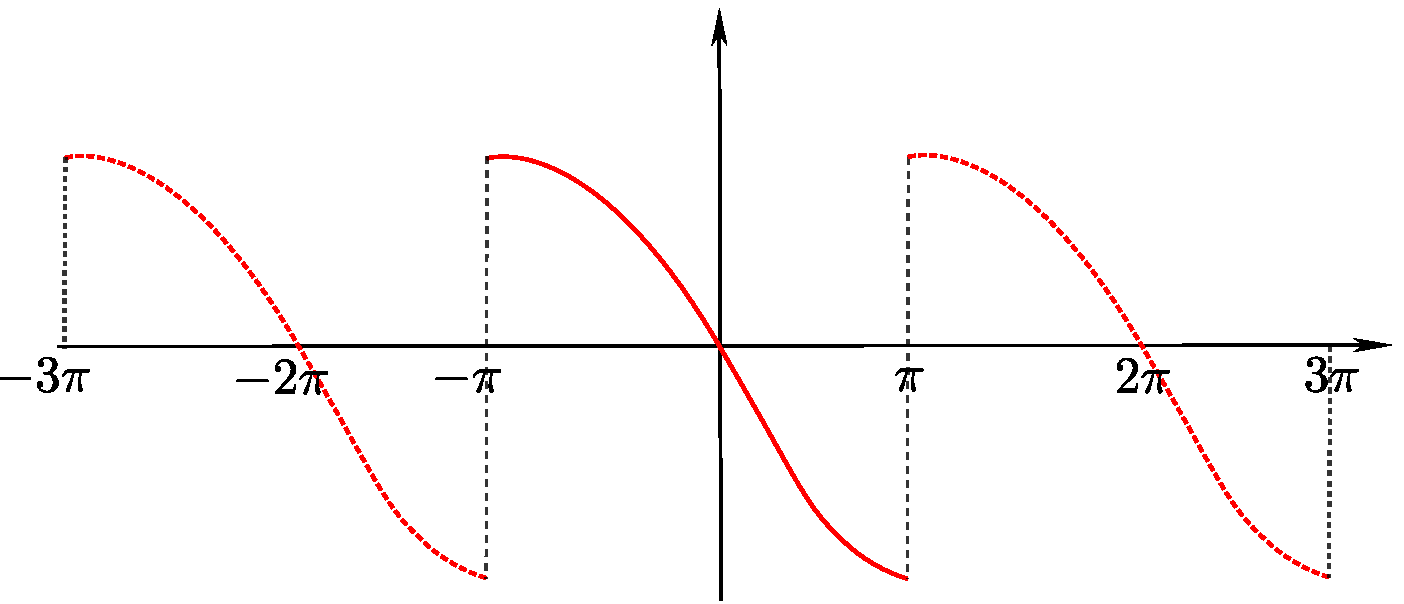
\includegraphics[scale = 0.45]{Figuras/Periocidad.pdf}
    \caption{Extensión periódica de una función real seccionalmente continua en $[-\pi,\pi]$.}
\end{figure}
\end{ejemplo}

\subsection{Funciones pares e impares}
 
\begin{defi}
Sea $f: [-a,a] \longrightarrow \mathbb{R}$ perteneciente a $\mathcal{C}[-a,a]$.
\vspace{-0.1cm}
\begin{align*}
    f ~\mbox{es par} &\Leftrightarrow \forall x \in [-a,a] :~ f(-t) = f(t). \\
    f ~\mbox{es impar} &\Leftrightarrow \forall x \in [-a,a] :~ f(-t) = -f(t).
\end{align*}
\end{defi} 

\textbf{Observación 1:} Sea $f: [-a,a] \longrightarrow \mathbb{R}$ integrable,
\begin{align*}
    f ~\mbox{es par} &\Rightarrow \int_{-a}^a f(t) \,dt = 2 \int_0^a f(t) \,dt. \\
    f ~\mbox{es impar} &\Rightarrow \int_{-a}^a f(t) \,dt = 0.
\end{align*}

\textbf{Observación 2:} Toda función $f:[-a,a] \longrightarrow \mathbb{R}$ puede expresarse como la suma de una función par más otra impar: $f = f_p + f_i$ con 
$$f_p(t) = \frac{f(t) + f(-t)}{2}, \quad f_i(t) = \frac{f(t) - f(-t)}{2}.$$

\begin{defi}
Sea $f \in \mathcal{C}[0,a]$ real, entonces la \textbf{extensión par} y la \textbf{extensión impar} de $f$ están definidas, respectivamente, por:
\begin{equation*}
    E_f(t) = \left\{ \begin{array}{cll}
    f(-t)     & \mbox{si} & -a \leq t < 0 \\
    f(t)     & \mbox{si} & 0 \leq t \leq a
    \end{array} \right. , ~ O_f(t) = \left\{ \begin{array}{cll}
    -f(-t)     & \mbox{si} & -a \leq t < 0 \\
    f(t)     & \mbox{si} & 0 \leq t \leq a
    \end{array} \right. .
\end{equation*}
\end{defi}

\begin{figure}[H]
    \centering
    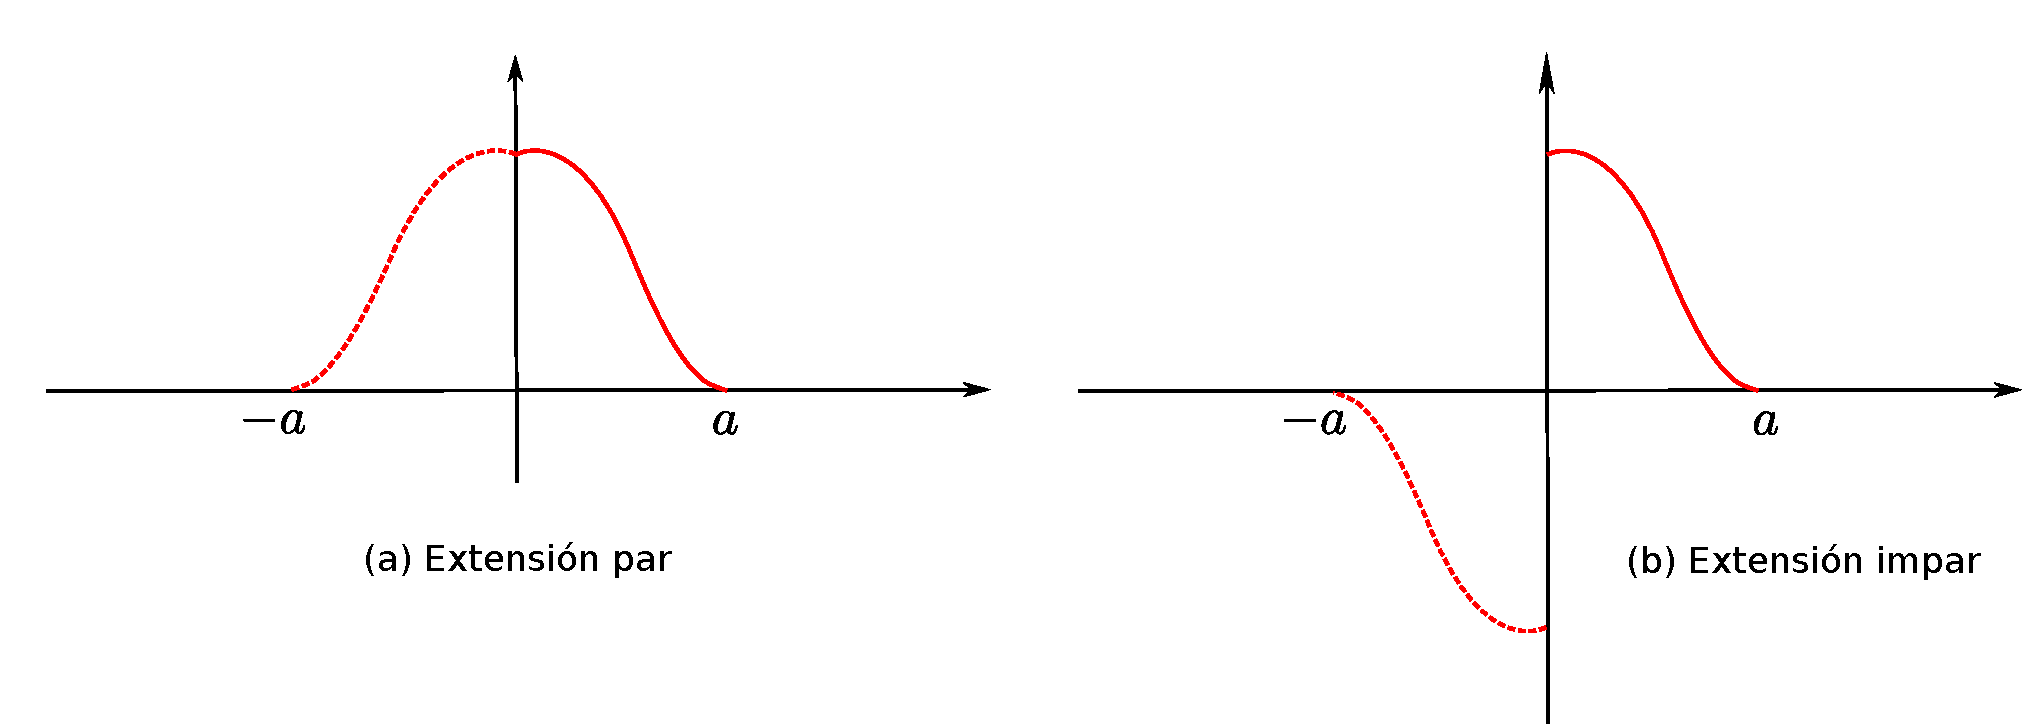
\includegraphics[scale = 0.45]{Figuras/Paridad.pdf}
    \caption{Extensión par e impar de una función real seccionalmente continua en $[0,a]$. }
\end{figure}

\section{Serie de Fourier trigonométrica}

\subsection{Definición}

En el espacio $\mathcal{C}[-\pi,\pi]$ consideremos el sistema ortonormal completo 
$$\left\{ \frac{1}{\sqrt{2\pi}}, \frac{\cos(nt)}{\sqrt{\pi}}, \frac{\sin(nt)}{\sqrt{\pi}} \right\}_{n=1}^{\infty}$$

llamado \textbf{sistema trigonométrico}.

\begin{defi}
Sea $f \in \mathcal{C}[-\pi,\pi]$, la serie 
\begin{equation}
    \frac{a_0}{2} + \sum_{n=1}^{\infty} ( a_n \cos(nt) + b_n \sin(nt)) \label{FourierTrigo}
\end{equation}

se denomina \textbf{serie trigonométrica de Fourier} o simplemente \textbf{serie de Fourier}, donde los \textit{coeficientes de Fourier} están dados por:
\begin{align*}
    a_0 &= \frac{1}{\pi} \int_{-\pi}^{\pi} f(t) \,dt, \\
    a_n &= \frac{1}{\pi} \int_{-\pi}^{\pi} f(t) \cos(nt) \,dt, \quad n = 1,2, \dots\\
    b_n &= \frac{1}{\pi} \int_{-\pi}^{\pi} f(t) \sin(nt) \,dt. \quad n = 1,2, \dots
\end{align*}
\end{defi}

\textbf{Observación}: La serie de Fourier de $f$ converge en media a $f$, o sea, 
\begin{shaded}
$$f(t) \sim \frac{a_0}{2} + \sum_{n=1}^{\infty} (a_n \cos(nt) + b_n \sin(nt)).$$    
\end{shaded}

\begin{propo} \label{C.FourierCero}
Los coeficientes de la serie trigonométrica de Fourier de $f \in \mathcal{C}[-\pi,\pi]$ convergen a cero cuando $n \to \infty$, es decir,
$$\lim_{n \to + \infty} a_n = \lim_{n \to + \infty} b_n = 0.$$
\end{propo}

\begin{demo}
Si denotamos el sistema trigonométrico por 
$$\varphi_0(t) = \frac{1}{\sqrt{2\pi}}, ~ \varphi_{2n-1}(t) = \frac{1}{\sqrt{\pi}} \cos(nt), ~ \varphi_{2n(t)} = \frac{1}{\sqrt{\pi}} \sin(nt), \quad n = 1,2, \dots$$

tenemos que la serie generalizada de Fourier queda
$$\sum_{n=0}^{\infty} C_n \varphi_n(t) = C_0 \varphi_0(t) + \sum_{n=1}^{\infty} \left[ C_{2n-1} \varphi_{2n-1}(t) + C_{2n} \varphi_{2n}(t) \right] ,$$

la cual corresponde a la serie trigonométrica de Fourier de $f \in \mathcal{C}[-\pi,\pi]$, donde 
$$a_0 = \sqrt{\frac{2}{\pi}} C_0, ~ a_n = \frac{C_{2n-1}}{\sqrt{\pi}}, ~ b_n = \frac{C_{2n}}{\sqrt{\pi}}, \quad n = 1,2, \dots$$

De lo discutido en el primer capítulo, una de las consecuencias de la desigualdad de Bessel \eqref{D.Bessel} es que 
$$\lim_{n \to + \infty} C_n = \lim_{n \to + \infty} \langle f, \varphi_n \rangle = 0 ~\Rightarrow~ \lim_{n \to \infty} C_{2n-1} = \lim_{n \to \infty} C_{2n} = 0. $$

Por lo tanto, 
$$\lim_{n \to + \infty} a_n = \lim_{n \to + \infty} b_n = 0.$$

\end{demo}

¿Convergerá puntual y/o uniformemente la serie de Fourier a $f(t)$? ¿Qué condiciones deben cumplirse?

Antes de responder estas preguntas, primero justifiquemos que es suficiente trabajar con funciones a valores reales, a pesar de que los siguientes teoremas también son válidos para funciones a valores complejos. 

Sea $f = u + iv \in \mathcal{C}[-\pi,\pi]$, su serie de Fourier trigonométrica está dada por \eqref{FourierTrigo} con 
\begin{align*}
    a_0 &= \frac{1}{\pi} \int_{-\pi}^{\pi} f(t) \,dt =  \frac{1}{\pi} \int_{-\pi}^{\pi} u(t) \,dt + \frac{i}{\pi} \int_{-\pi}^{\pi} v(t) \,dt,\\
    a_n &= \frac{1}{\pi} \int_{-\pi}^{\pi} f(t) \cos(nt) \,dt = \frac{1}{\pi} \int_{-\pi}^{\pi} u(t) \cos(nt) \,dt + \frac{i}{\pi} \int_{-\pi}^{\pi} v(t) \cos(nt) \,dt , \quad n = 1,2, \dots\\
    b_n &= \frac{1}{\pi} \int_{-\pi}^{\pi} f(t) \sin(nt) \,dt = \frac{1}{\pi} \int_{-\pi}^{\pi} u(t) \sin(nt) \,dt + \frac{i}{\pi} \int_{-\pi}^{\pi} v(t) \sin(nt) \,dt, \quad n = 1,2, \dots
\end{align*}

Entonces, su serie de Fourier nos queda
\begin{align*}
  f(t) & \sim   \left\{ \frac{Re(a_0)}{2} + \sum_{n=1}^{\infty} ( Re(a_n) \cos(nt) + Re(b_n) \sin(nt) ) \right\}  \\
   &  + i \left\{ \frac{Im(a_0)}{2} + \sum_{n=1}^{\infty} (Im(a_n) \cos(nt) + Im(b_n) \sin(nt)) \right\},
\end{align*}

es decir, la serie de Fourier de $f = u + iv$ es la de $u(t) + i$ (la de $v(t)$). 

\subsection{Series de senos y cosenos}

Sea $f:[0,\pi] \longrightarrow \mathbb{R}$ seccionalmente continua, entonces la extensión par e impar de $f$ están definidas por:
\begin{equation*}
    E_f(t) = \left\{ \begin{array}{cll}
    f(-t)     & \mbox{si} & -\pi \leq t < 0 \\
    f(t)     & \mbox{si} & 0 \leq t \leq \pi
    \end{array} \right. , ~ O_f(t) = \left\{ \begin{array}{cll}
    -f(-t)     & \mbox{si} & -\pi \leq t < 0 \\
    f(t)     & \mbox{si} & 0 \leq t \leq \pi
    \end{array} \right. .
\end{equation*}

Puesto que $E_f, O_f: [-\pi,\pi] \longrightarrow$ son seccionalmente continuas, se puede obtener el desarrollo en serie de Fourier de éstas, los cuales están definidos por: \footnote{La forma de las series seno y coseno, con sus respectivos coeficientes, se obtienen al aplicar las propiedades vistas para las funciones pares e impares.}
$$ E_f(t) \sim \frac{a_0}{2}  + \sum_{n=1}^{\infty} a_n \cos(nt), ~~\mbox{donde}~~ a_n = \frac{2}{\pi} \int_0^{\pi} f(t) \cos(nt)\,dt$$

y
$$ O_f(t) \sim  \sum_{n=1}^{\infty} b_n \sin(nt), ~~\mbox{donde} ~~ b_n = \frac{2}{\pi} \int_0^{\pi} f(t) \sin (nt)\,dt.$$

Estos son llamados \textbf{desarrollos en serie de Fourier de coseno y de seno de $f$}, respectivamente.

\subsection{Convergencia puntual y uniforme}

\begin{defi}
Sea $f: [a,b] \longrightarrow \mathbb{R}$, para $t_0 \in [a,b]$ definimos
\begin{align*}
    f(t_0^+) &= \lim_{t \to t_0^+} f(t), \\
    f(t_0^-) &= \lim_{t \to t_0^-} f(t),
\end{align*}

si existen los límites. 

Una discontinuidad en $t_0$ tal que $f(t_0^+)$ y $f(t_0^-)$ existen se denomina \textbf{discontinuidad de salto} y $f(t_0^+) - f(t_0^-)$ recibe el nombre de \textbf{salto} de $f$ en $t_0$.
\end{defi}

\textbf{Observaciones:} 

\begin{enumerate}
    \item La magnitud del salto es $|f(t_0^+) - f(t_0^-)|$.
    
    \item El salto se anula cuando $f(t_0) = f(t_0^+) = f(t_0^-)$, es decir, cuando $f$ es continua en $t_0$.
    
    \item Una función $f: [a,b] \longrightarrow \mathbb{R}$ seccionalmente continua tiene discontinuidades de salto.
\end{enumerate}

\begin{defi}
Sea $f:[a,b] \longrightarrow \mathbb{R}$, con una discontinuidad de salto en $t_0 \in [a,b]$, definimos la \textbf{derivada por la derecha} como 
$$f'(t_0^+) = \lim_{h \to 0^+} \frac{f(t_0 + h ) - f(t_0^+)}{h}$$

cuando el límite existe. Similarmente, definimos la \textbf{derivada por la izquierda} como 
$$f'(t_0^-) = \lim_{h \to 0^-} \frac{f(t_0 + h ) - f(t_0^-)}{h}$$

cuando el límite existe.
\end{defi}

\begin{teorema}[Convergencia puntual de la serie de Fourier] \label{Puntual}
Sea $f(t)$ una función real seccionalmente continua en el intervalo $-\pi < t < \pi$. Su serie de Fourier trigonométrica converge al valor medio
\vspace{-0.05cm}
$$\frac{f(t^+) + f(t^-)}{2}$$

para cada $t \in (-\pi,\pi)$ donde ambas derivadas laterales $f'(t^+)$ y $f'(t^-)$ existen.
\end{teorema}

\begin{demo}
    Consultar la sección \ref{DemostracionesFourier}
\end{demo}

\textbf{Observación:} Si denotamos por $f_e$ a la extensión periódica de $f$, a partir del teorema anterior, la expansión en serie de Fourier converge a $f_e$ para todo $x \in \mathbb{R}$ al extenderla periódicamente al valor medio
$$\frac{f_e(t^+) + f_e(t^-)}{2}.$$

De hecho, en los extremos $t = \pm \pi$, la serie converge a 
$$\frac{f(-\pi^+) + f(\pi^-)}{2}.$$

En efecto, observemos que
$$f_e(-\pi^+) = f(-\pi^+) ~~\mbox{y}~~ f_e(-\pi^-) = f(\pi^-).$$

Luego, el cociente
$$\frac{f_e(-\pi^+) + f_e(-\pi^-)}{2} = \frac{f(-\pi^+) + f(\pi-)}{2}.$$

Análogamente para $t = \pi$.

\begin{teorema}[Convergencia uniforme] \label{C.Uniforme}
Supóngase que $f$ es continua en $[-\pi,\pi]$, $f(-\pi) = f(\pi)$ y que $f'$ es continua por tramos, con discontinuidades de salto. Entonces la serie de Fourier trigonométrica de $f$ converge a $f$ absolutamente y uniformemente.
\end{teorema}

\begin{demo}
    Consultar la sección \ref{DemostracionesFourier}
\end{demo}

\subsection{Ejemplos}

\begin{ejemplo} \label{EjemploFourier1}
Consideremos la función $f(x) = x^2$ definida para $x\in [-\pi,\pi]$, la cual es continua con derivada $f'(x) = 2x$ también continua, luego la serie de Fourier de $f$ converge puntualmente a $f$ para todo $x \in (-\pi,\pi)$. Para los extremos $x = \pm \pi$ vemos que $f(\pi) = f(-\pi)$, por lo tanto la serie converge puntualmente a $f$ para todo $x \in [-\pi,\pi]$.

Sus coeficientes de Fourier están dados por:
\begin{align*}
    a_0 &= \frac{1}{\pi} \int_{-\pi}^{\pi} x^2 \,dx = \left. \frac{x^3}{3\pi} \right|_{-\pi}^{\pi} = \frac{2}{3} \pi^2, \\
    a_n &= \frac{1}{\pi} \int_{-\pi}^{\pi} x^2 \cos(n x)\,dx =   \left. \frac{1}{n\pi} x^2 \sin(nx)  \right|_{-\pi}^{\pi} - \frac{2}{n\pi} \int_{-\pi}^{\pi} x \sin(nx) \,dx\\
    &= \left.   \frac{2}{n^2\pi} x \cos(nx)\right|_{-\pi}^{\pi} - \frac{2}{n^2 \pi} \cancelto{0}{\int_{-\pi}^{\pi} \cos(nx) \,dx }\\
    &=  \frac{4}{n^2} \cos(n\pi) =  (-1)^n \frac{4}{n^2}, \quad n = 1,2,\dots\\
     b_n &= \frac{1}{\pi} \int_{-\pi}^{\pi} x^2 \sin(nx)\,dx = 0, \quad n = 1,2, \dots
\end{align*}

Entonces, su serie de Fourier es
\begin{equation}
f(x) = \frac{\pi^2}{3} + \sum_{n=1}^{\infty} (-1)^n \frac{4}{n^2} \cos(nx), \qquad x \in [-\pi,\pi].    \label{FourierCuadratica}
\end{equation}

Es claro que la serie de Fourier de $f(x) = x^2$ para todo $x\in \mathbb{R}$ representa la extensión periódica de los valores de $f(x)$ en el intervalo $[-\pi,\pi]$.

La gráfica de $f$ en conjunto con diferentes sumas parciales de su serie de Fourier están representadas en la figura \ref{fig:EjemploFourier1}. 

\begin{figure}[H]
    \centering
    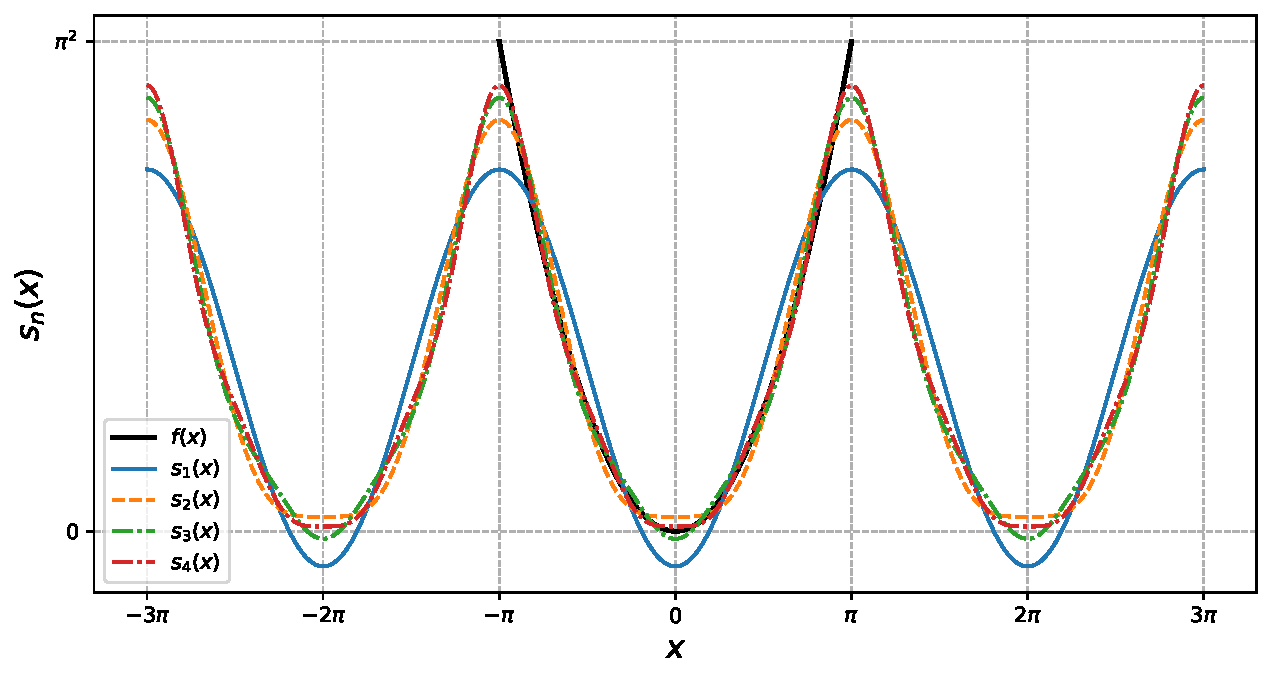
\includegraphics[scale = 0.65]{Figuras/EjemploFourier1.pdf}
    \caption{Serie de Fourier de la función $f(x) = x^2, -\pi \leq x \leq \pi$, truncada hasta $n = 4$.}
    \label{fig:EjemploFourier1}
\end{figure}

El teorema visto para convergencia uniforme nos garantiza que esta serie converge uniformemente a $f(x) = x^2$ en $[-\pi,\pi]$, es más, al aplicar el criterio de M de Weierstrass a la serie, ésta converge para todo $x \in \mathbb{R}$, pues
$$\forall  x \in \mathbb{R}: ~ \left|(-1)^n \frac{4}{n^2} \cos(nx)\right| \leq \frac{4}{n^2} = M_n ~~\mbox{y}~~  \sum\limits_{n=1}^{\infty} M_n < \infty.$$

\end{ejemplo}

Podemos usar la expansión en serie de Fourier de $f(x) = x^2$ en $[-\pi,\pi]$ para probar que 
$$\sum_{n=1}^{\infty} \frac{1}{n^2} = 1 + \frac{1}{4} + \frac{1}{9} + \cdots = \frac{\pi^2}{6}.$$

En efecto, al evaluar $x = \pi$ en \eqref{FourierCuadratica}, obtenemos que 
$$f(\pi) = \frac{\pi^2}{3} + \sum_{n=1}^{\infty} (-1)^n \frac{4}{n^2} \cos(n\pi) = \frac{\pi^2}{3} + \sum_{n=1}^{\infty} (-1)^{2n} \frac{4}{n^2} = \frac{\pi^2}{3} +  \sum_{n=1}^{\infty} \frac{4}{n^2}.$$

Así,
$$\pi^2 = \frac{\pi^2}{3} + 4 \sum_{n=1}^{\infty} \frac{1}{n^2} \Rightarrow \sum_{n=1}^{\infty} \frac{1}{n^2} = \frac{\pi^2}{6}.$$

\begin{ejemplo} \label{Signo}
Consideremos la función signo  definida por
$$f(x) := \left\{ \begin{array}{cc}
     -1,& - \pi \leq x < 0  \\
     1,&   0 \leq x \leq \pi
\end{array} \right. .$$

La función es seccionalmente continua con $x = 0$ punto de discontinuidad de salto y las derivadas laterales existen para todo $x \in (-\pi,\pi)$, luego la serie de Fourier de $f$ converge puntualmente a $f$ en los puntos de continuidad y a 
$$\frac{f(0^-) + f(0^+)}{2} = 0, \quad \mbox{en} ~ x = 0 ~~\mbox{y}$$
$$\frac{f(-\pi^+) + f(\pi^-)}{2} = 0, \quad \mbox{en} ~ x = \pm \pi. $$

Sus coeficientes de Fourier están dados por:
\begin{align*}
    a_0 &= \frac{1}{\pi} \int_{-\pi}^{\pi} f(x) \,dx = 0 , \\
    a_n &= \frac{1}{\pi} \int_{-\pi}^{\pi} f(x) \cos(n x)\,dx = 0, \quad n = 1,2,\dots
\end{align*}
\begin{align*}
     b_n &= \frac{1}{\pi} \int_{-\pi}^{\pi} f(x) \sin(nx) \,dx \\
     &= \frac{1}{\pi} \int_{-\pi}^0 (-1) \sin(nx)\,dx + \frac{1}{\pi} \int_{0}^{\pi} (1) \sin(nx) \,dx \\
     &= \left.  \frac{1}{\pi n} \cos(nx) \right|_{-\pi}^0 - \left. \frac{1}{\pi n} \cos(nx) \right|_{0}^{\pi} \\
     &= \frac{2}{\pi n} [1 - (-1)^n] \\
     &= \left\{ \begin{array}{cl}
         0, & n ~\mbox{par}  \\
         \frac{4}{\pi n}, &  n ~\mbox{impar}
     \end{array} \right. .
\end{align*}

Entonces, su serie de Fourier es 
$$f(x) =  \sum_{n ~impar} \frac{4}{\pi n} \sin(nx) = \sum_{k=1}^{\infty} \frac{4}{\pi} \frac{\sin[(2k-1)x]}{ (2k-1)}.$$

\textbf{Aclaración:} Note que a pesar de haber escrito que la función $f$ es igual a la serie, debemos tener en cuenta que en los punto $x = 0$ y $x = \pm \pi$ converge al valor medio del salto de la discontinuidad.

Es claro que la serie de Fourier de $f$ para todo $x\in \mathbb{R}$ representa la extensión periódica de los valores de $f(x)$ en el intervalo $[-\pi,\pi]$.

La gráfica de $f$ en conjunto con diferentes sumas parciales de su serie de Fourier están representadas en la figura \ref{fig:EjemploFourier2}.

\begin{figure}[H]
    \centering
    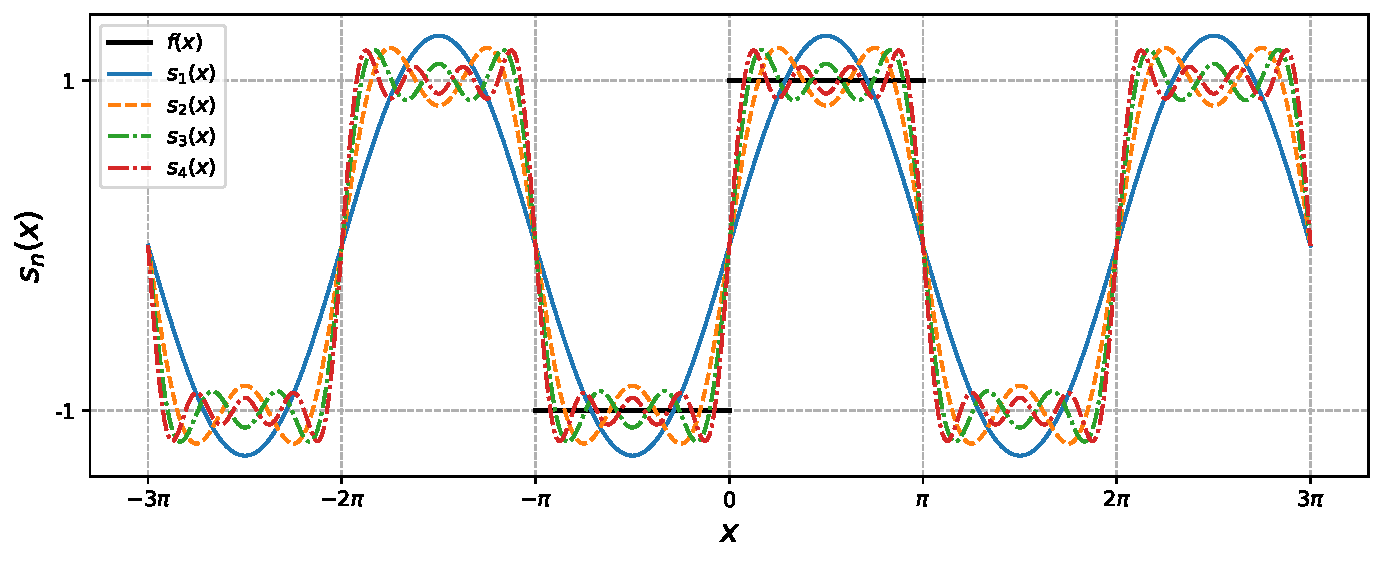
\includegraphics[scale = 0.65]{Figuras/EjemploFourier2.pdf}
    \caption{Serie de Fourier de la función signo truncada hasta $n = 4$.}
     \label{fig:EjemploFourier2}
\end{figure}

\end{ejemplo}

\section{Serie exponencial}

En el espacio $\mathcal{C}[-\pi,\pi]$ consideremos el sistema ortonormal completo 
$$\left\{ \frac{1}{\sqrt{2\pi}} e^{int} \right\}_{n= - \infty}^{n = \infty}$$

llamado \textbf{sistema exponencial}.

\begin{defi}
Sea $f \in \mathcal{C}[-\pi,\pi]$, la serie 
\begin{equation}
     \sum_{n=- \infty}^{\infty} c_n e^{int} \label{FourierExpo}
\end{equation}

se denomina \textbf{serie exponencial de Fourier}  donde los \textit{coeficientes de Fourier} están dados por:
\begin{equation*}
    c_n = \frac{1}{2\pi} \int_{-\pi}^{\pi} f(t) e^{-int} \,dt.
\end{equation*}
\end{defi}

\textbf{Observación}: La serie de Fourier de $f$ converge en media a $f$, o sea, 
\begin{shaded}
 $$f(t) \sim \sum_{n=- \infty}^{\infty} c_n e^{int}.$$   
\end{shaded}

\begin{propo} \label{TrigoExpo}
La $n$-ésima suma parcial de la serie de Fourier trigonométrica de una función (real o compleja) es igual a la $n$-ésima suma parcial de la serie exponencial.
\end{propo}

\begin{demo}
La $n$-ésima suma parcial de la serie exponencial es
$$ s_n(t) = \sum_{k=-n}^n c_k e^{ikt}.$$

Separando la suma:
\begin{align*}
    s_n(t) &= \sum_{k=-n}^{-1} c_k e^{ikt} + c_0 + \sum_{k=1}^n c_k e^{ikt} \\
    &= c_0 + \sum_{k=1}^n c_k e^{ikt} + \sum_{k=1}^n c_{-k} e^{-ikt} \\
    &= c_0 + \sum_{k=1}^n [c_k e^{ikt} + c_{-k} e^{-ikt}]. 
\end{align*}

Usando la identidad de Euler, $e^{i\theta} = \cos(\theta) + i \sin(\theta)$, encontramos que
$$s_n(t) = c_0 +  \sum_{k=1}^n [(c_k + c_{-k}) \cos(kt) + i(c_k - c_{-k}) \sin(kt)].$$

Desarrollando los coeficientes de la serie exponencial de Fourier, tenemos que
\begin{align*}
    c_0 &= \frac{1}{2\pi} \int_{-\pi}^{\pi} f(t) \,dt, \\
    c_k + c_{-k} &= \frac{1}{2\pi} \int_{-\pi}^{\pi} f(t) e^{-ikt} \,dt + \frac{1}{2\pi} \int_{-\pi}^{\pi} f(t) e^{ikt} \,dt  \\
    &= \frac{1}{2\pi} \int_{-\pi}^{\pi} f(t) [e^{ikt} + e^{-ikt}] \,dt \\
    &= \frac{1}{\pi} \int_{-\pi}^{\pi} f(t) \cos(kt) \,dt; \quad k = 1,2, \dots\\
   i( c_k - c_{-k}) &= \frac{i}{2\pi} \int_{-\pi}^{\pi} f(t) e^{-ikt} \,dt - \frac{i}{2\pi} \int_{-\pi}^{\pi} f(t) e^{ikt} \,dt \\
   &= - \frac{i}{2\pi} \int_{-\pi}^{\pi} f(t) [e^{ikt} - e^{-ikt}] \,dt \\
   &= \frac{1}{\pi} \int_{-\pi}^{\pi} f(t) \sin(kt)\,dt; \quad k = 1,2, \dots
\end{align*}

Comparando las expresiones obtenidas con los coeficientes de la serie de Fourier trigonométrica, podemos concluir que 
$$c_0 = \frac{a_0}{2}, ~  c_k + c_{-k} = a_k, ~ i( c_k - c_{-k}) = b_k; \quad k = 1,2, \dots$$

Por lo tanto, 
$$ s_n(t) = \sum_{k=-n}^n c_k e^{ikt} = \frac{a_0}{2} + \sum_{k=1}^n (a_k \cos(kt) + b_k \sin(kt)).$$

\end{demo}

\textbf{Observación 1:} Una consecuencia inmediata de la proposición \ref{TrigoExpo} es que todos los teoremas vistos para la serie de Fourier trigonométrica son aplicables a la serie de Fourier exponencial.
\\

\textbf{Observación 2:} Los coeficientes de las series \eqref{FourierTrigo} y \eqref{FourierExpo} están relacionados por 
\begin{equation}
a_0 = 2c_0,~~ a_n = c_n + c_{-n}, ~~ b_n = i(c_n - c_{-n}); \quad n = 1,2, \dots    \label{RelacionCoefi1}
\end{equation}

o bien, 
\begin{equation}
    c_n = \left\{ \begin{array}{cl}
        \frac{1}{2} (a_n - ib_n), & n \geq 0  \\
    \frac{1}{2}(a_{-n} + i b_{-n}),     & n  \leq -1 
    \end{array} \right. . \label{RelacionCoefi2}
\end{equation}

Si $f(t)$ es una función real, entonces sus respectivos coeficientes complejos $c_n$ satisfacen la relación:
$$c_n^* = \frac{1}{2\pi} \int_{-\pi}^{\pi} f(t) (e^{-int})^* \,dt = \frac{1}{2\pi} \int_{-\pi}^{\pi} f(t) e^{int} \,dt = c_{-n}.$$

\section{Diferenciación e integración de las series de Fourier}

Supongamos que tenemos una serie de funciones
$$\sum_{n=1}^{\infty} f_n(t),$$

y queremos integrarla (o derivarla). Resulta tentador intercambiar la integral (o derivada) por la serie, es decir, integrar (o derivar) término a término. Sin embargo, este intercambio no es siempre posible porque puede romper la convergencia de la serie. Por ejemplo, las series de potencia se pueden integrar (o derivar) término a término en su región de convergencia sin problema. En nuestro caso, nos interesa saber que condiciones deben cumplirse para las series de Fourier.

\begin{teorema}[Integración]
Sea $f$ una función seccionalmente continua en el intervalo $-\pi < t < \pi$. Independiente si la serie \eqref{FourierTrigo} converge, la siguiente ecuación es válida cuando $-\pi \leq t \leq \pi$:
\begin{equation*}
  \int_{-\pi}^t f(s) \,ds = \frac{a_0}{2} (t + \pi) + \sum_{n=1}^{\infty} \frac{1}{n} \left\{ a_n \sin(nt) - b_n[\cos(nt) + (-1)^{n+1}] \right\}.   
\end{equation*}
\end{teorema}

\begin{demo}
Consultar la sección \ref{DemostracionesFourier}.
\end{demo}

\begin{teorema}[Derivación]
Sea $f$ una función continua en $[-\pi,\pi]$, donde $f(-\pi) = f(\pi)$, y $f'$ es seccionalmente continua en el intervalo $(-\pi,\pi)$. Entonces, la serie de Fourier
\begin{equation*}
    f(t) = \frac{a_0}{2} + \sum_{n=1}^{\infty} (a_n \cos(nt) + b_n \sin (nt) ), \quad t \in [-\pi,\pi],
\end{equation*}

donde 
$$a_n = \frac{1}{\pi} \int_{-\pi}^{\pi} f(t) \cos(nt) \,dt, \quad b_n = \frac{1}{\pi} \int_{-\pi}^{\pi} f(t) \sin(nt) \,dt,$$

es derivable para todo $t \in (-\pi,\pi)$ en el cual $f''(t)$ existe:
\begin{equation*}
    f'(t) = \sum_{n=1}^{\infty} (- n a_n \sin(nt) + nb_n \cos(nt)).
\end{equation*}
\end{teorema}

\begin{demo}
Consultar la sección \ref{DemostracionesFourier}.
\end{demo}

\begin{ejemplo}
Obtener el desarrollo en serie de Fourier de la función $x^3$ en el intervalo $[-\pi,\pi]$.
\\

\textbf{Solución}: Las funciones del tipo $x^n$, $n \in \mathbb{N}$ son continuas, derivables e integrables, por lo que podemos aplicar estas operaciones a las series de Fourier que se obtengan a partir de ellas.  En nuestro caso obtendremos el desarrollo de $x^3$ por integración de $x^2$, cuyo desarrollo en serie de Fourier ya obtuvimos en el ejemplo \ref{EjemploFourier1}:
\begin{align*}
   \forall x \in [-\pi,\pi]:  \int_{-\pi}^x t^2 \,dt &=   \int_{-\pi}^x   \frac{\pi^2}{3} + \sum_{n=1}^{\infty} (-1)^n \frac{4}{n^2} \cos(nt) \,dt\\
    \Rightarrow ~ \frac{x^3}{3} + \frac{\pi^3}{3} &=  \frac{\pi^2}{3} (x+\pi) + \sum_{n=1}^{\infty} (-1)^n \frac{4 }{n^3}  \sin(nx)  \\
\Rightarrow \qquad \quad    x^3 &= \pi^2 x + 12 \sum_{n=1}^{\infty} \frac{(-1)^n}{n^3} \sin(nx).
\end{align*}

Lo que obtuvimos es el desarrollo en serie de $x^3-\pi^2 x$. Para obtener el desarrollo de $x^3$, encontremos la serie de Fourier de $x$, para ello utilicemos el desarrollo de $x^2$, pero esta vez derivando:
\begin{align*}
    \frac{d}{dx} [x^2] &= \frac{d}{dx} \left[  \frac{\pi^2}{3} + \sum_{n=1}^{\infty} (-1)^n \frac{4}{n^2} \cos(nx)\right] \\
   \Rightarrow \qquad 2x &= - \sum_{n=1}^{\infty} (-1)^n \frac{4}{n} \sin(nx) \\
   \Rightarrow \qquad ~ x &= - 2 \sum_{n=1}^{\infty}  \frac{(-1)^n}{n} \sin(nx).
\end{align*}

Sustituyendo en $x^3$:
\begin{align*}
    x^3 &= -2 \pi^2 \sum_{n=1}^{\infty}  \frac{(-1)^n}{n} \sin(nx) + 12 \sum_{n=1}^{\infty} \frac{(-1)^n}{n^3} \sin(nx) \\
    &= \sum_{n=1}^{\infty} \frac{(-1)^n}{n^3} \left[ 12 - 2\pi^2 n^2 \right] \sin(nx).
\end{align*}
\end{ejemplo}

\section{Fenómeno de Gibbs}

Cuando queremos aproximar una función $f$ con las sumas parciales de su serie de Fourier, se puede observar un comportamiento particular cerca de los puntos de discontinuidad aislados, por ejemplo, al graficar la serie de Fourier de la función signo para un $n$ alto, ver figura \ref{fig:GibssSign}, se comete un error considerable en las cercanías al punto de discontinuidad, y además este
error no disminuye si se incluyen más términos en la serie. Este efecto indeseado se denomina \textbf{fenómeno de Gibbs}. 

\begin{figure}[H]
    \centering 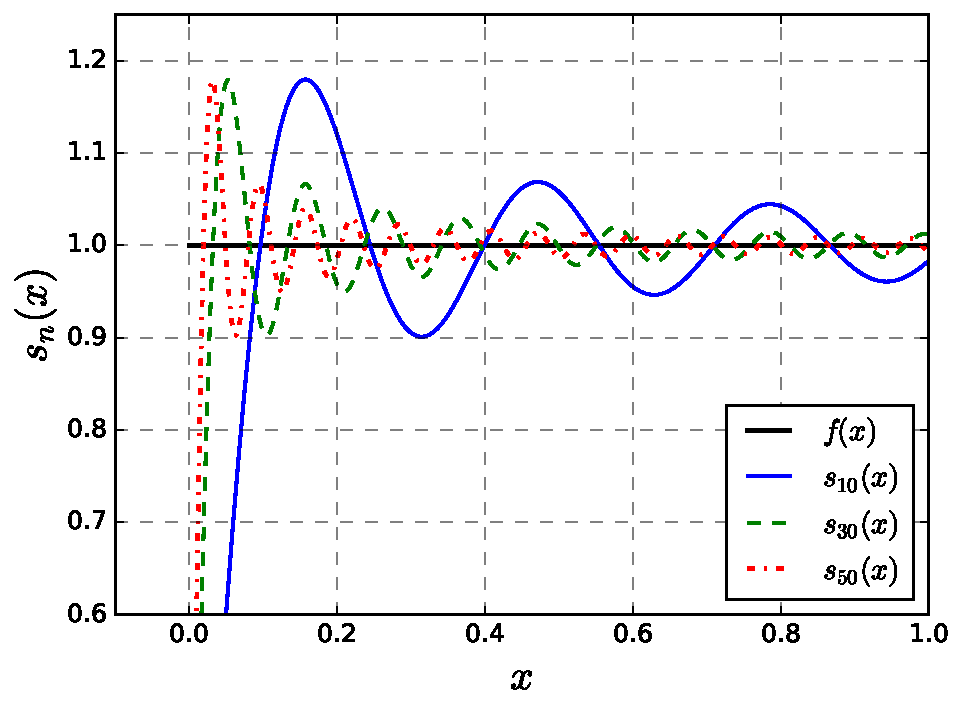
\includegraphics[scale = 0.65]{Figuras/FenomenoGibbs.pdf}
    \caption{Fenómeno de Gibbs en la función signo para $n = 10,30,50$.}
    \label{fig:GibssSign}
\end{figure}

Ilustremos este hecho con un análisis analítico de la función ya estudiada
$$f(x) = \left\{ \begin{array}{cc}
     -1,& - \pi \leq x < 0  \\
     1,&   0 \leq x \leq \pi
\end{array} \right. .$$

Su serie de Fourier está dada por
$$\sum_{n=1}^{\infty} \frac{4}{\pi} \frac{\sin[(2n-1)x]}{ (2n-1)}.$$

Sea 
$$s_n(x) = \frac{4}{\pi} \sum_{k=1}^n \frac{\sin[(2k-1)x]}{2k-1}$$

su $n$-ésima suma parcial. Derivando y multiplicando por $\pi \sin(x)$, encontramos que 
\begin{align*}
   \pi (\sin x)s_n'(x) =4 \sin(x) \sum_{k=1}^n \cos[(2k-1)x] &= 4 \sum_{k=1}^n   \sin(x) \cos[(2k-1)x] \\
   &= 4 \sum_{k=1}^n  \frac{1}{2}[\sin(x + (2k-1)x) + \sin(x - (2k-1)x)] \\
   &= 2 \sum_{k=1}^n [\sin(2k x) - \sin([2k-2]x)] \\
   &= 2 \sin(2nx).
\end{align*}

Luego, 
\begin{equation*}
  2 \sin(2nx_c) = 0 ~\Leftrightarrow~ x_c = \frac{m \pi}{2n}, \quad m \in \mathbb{Z}. 
\end{equation*}

Nos interesa encontrar el primer máximo de $s_n(x)$, así que tomaremos los valores $m = \pm 1$ de prueba, pues en $m = 0$ no se alcanza un máximo dado que $s_n(0) = 0$. Como $\sin(x_c) \neq 0$, para estos valores de $m$,  $s_n'(x_c) = 0$ y, en consecuencia, $x_c$ son los puntos críticos de $s_n$. 

En la siguiente tabla se analizan los signos de $s_n'(x)$.

\begin{figure}[H]
    \centering
    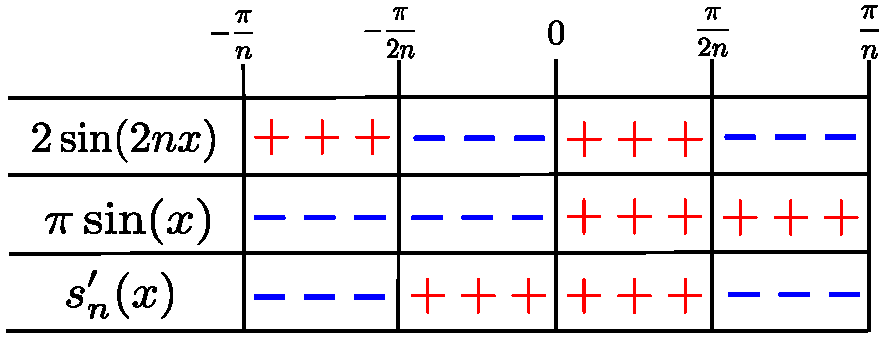
\includegraphics[scale = 0.62]{Figuras/EjemploGibbs.pdf}
    \caption{Tabla con el análisis de signos de $s_n'(x)$ asociada a la función signo.}
\end{figure}

Por el criterio de la primera derivada, vemos que $s_n$ tiene un máximo en $x_n = \frac{\pi}{2n}$. El valor de ese máximo es
$$s_n \left( \frac{\pi}{2n}\right) = \frac{4}{\pi} \sum_{k=1}^n \frac{\sin[(2k-1)\pi/2n]}{2k-1} = \frac{2}{\pi} \sum_{k=1}^n \frac{\sin[(2k-1)\pi /2n]}{(2k-1) \pi/2n} \left(\frac{\pi}{n} \right).$$

Notemos que la sumatoria 
$$ \sum_{k=1}^n \frac{\sin[(2k-1)\pi /2n]}{(2k-1) \pi/2n} \left(\frac{\pi}{n} \right)$$

es una suma de Riemann para la función $\sin y/y$ en $[0,\pi]$ para la partición regular $0 = x_0 < x_1  <  \cdots< x_n =  \pi$ con $x_i = (\pi/n) i$, $i = 0,1, \dots, n$ y eligiendo el punto medio de cada intervalo $[x_{k-1},x_k]$,
$$ \frac{x_{k-1} + x_k}{2} = (2k-1) \frac{\pi}{2n}, \quad  k = 1, \dots, n,$$

para evaluar $\sin y/y$. Entonces, 
$$\int_0^{\pi} \frac{\sin y}{y} \,dy \approx \frac{\pi}{2} s_n\left( \frac{\pi}{2n}\right).$$

Como 
$$\int_0^{\pi} \frac{\sin y}{y} \,dy ~~ \mbox{converge} ~\Rightarrow~ \lim_{n \to + \infty} s_n\left( \frac{\pi}{2n} \right) = \frac{2}{\pi} \int_0^{\pi} \frac{\sin y}{y} \,dy.$$

Usando un método numérico de integración (o su calculadora de integrales favorita), se tiene que 
$$\int_0^{\pi} \frac{\sin y}{y} \,dy \approx 1.85193\dots$$

Por lo tanto, 
$$\lim_{n \to + \infty} s_n\left( \frac{\pi}{2n} \right) \approx 1.179.$$

Así, las aproximaciones exceden el valor real de $f(0^+) = 1$ por $0.179$ o $8.95\%$ del salto de $f(0^-)$ a $f(0^+)$. 
\\

En general, se puede demostrar el siguiente teorema, debido a M. B$\hat{\mbox{o}}$cher \cite{Bôcher}:

\begin{teorema}
Sea $f$ una función de variable real, con período $2\pi$. Supongamos que $f$ y $f'$ son ambas continuas excepto para un número finito de discontinuidades de salto en el intervalo $[-\pi,\pi]$. Sea $s_n(x)$ la suma parcial de orden $n$ de Fourier. Entonces, en un punto $a$ de discontinuidad, las gráficas de las funciones $s_n(x)$ convergen al segmento vectical (ver figura \ref{Gibbs}) de longitud 
$$L = \frac{2}{\pi} Si(\pi) |f(a^+) - f(a^-)| \approx 1.179 |f(a^+) - f(a^-)|$$

centrada en el punto 
$$\left(a, \frac{f(a^+) + f(a^-)}{2} \right),$$

donde 
$$Si(x) = \int_0^x \frac{\sin t}{t} \,dt$$

es la función seno integral.
\end{teorema}

\begin{figure}[H]
    \centering
    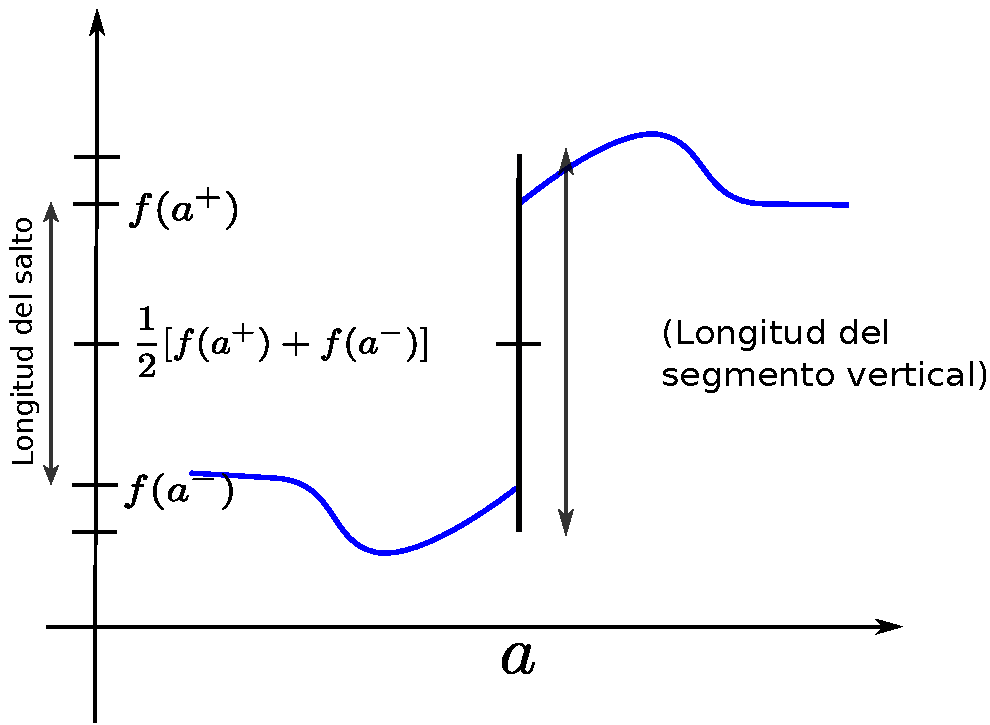
\includegraphics[scale = 0.55]{Figuras/Gibbs.pdf}
    \caption{Fenómeno de Gibbs en un punto de discontinuidad. Adaptado de \cite{UFRO}, pág. 202.}
    \label{Gibbs}
\end{figure}
 
\section{Cambio de intervalo}

Hasta ahora hemos estudiado funciones en el intervalo $[-\pi,\pi]$, sin embargo, es posible extender los resultados al caso de funciones seccionalmente continuas en un intervalo más general $[a,b]$. 

Sea $f \in \mathcal{C}[a,b]$, consideremos $\alpha: [- \pi,\pi] \longrightarrow [a,b]$ definida por \footnote{El lector puede llegar a esta función calculando la ecuación de la recta que pasa por los puntos $(-\pi,a)$ y $(\pi,b)$. La función resultante mapea biunívocamente los puntos del intervalo $[-\pi,\pi]$ a $[a,b]$.} 
$$\alpha(t) = a + \frac{b-a}{2\pi} (t+\pi)$$

la cual es continua, creciente con $\alpha(-\pi) = a$ y $\alpha(\pi) = b$. Ahora, si consideramos la función compuesta $g = f \circ \alpha$, se tiene que $g \in \mathcal{C}[-\pi,\pi]$. Luego, 
$$g(t) \sim \sum_{n= - \infty}^{\infty} c_n e^{int}$$

donde 
$$c_n = \frac{1}{2\pi} \int_{-\pi}^{\pi} g(t) e^{-int} \,dt, \quad n \in \mathbb{Z}.$$

Al hacer 
$$x = a + \frac{b-a}{2\pi} (t+\pi) ~\Leftrightarrow~ t = \frac{2x-b-a}{b-a} \pi = \frac{2 \pi}{b-a} x - \frac{b+a}{b-a} \pi  ,$$

se obtiene $g(t) = f(a + \frac{b-a}{2\pi} (t+\pi)) = f(x)$ y así 
$$f(x) \sim \sum_{n=-\infty}^{\infty} c_n \left[ e^{i\frac{2n\pi}{b-a} x} e^{-i \frac{b+a}{b-a}n\pi}\right].$$

Haciendo el cambio de variable $t = \frac{2\pi}{b-a} x - \frac{b+a}{b-a} \pi ~\Rightarrow~ dt = \frac{2\pi}{b-a} dx$, se obtiene
\begin{align*}
 c_n = \frac{1}{2\pi} \int_{-\pi}^{\pi} f(a + \frac{b-a}{2\pi} (t+\pi)) e^{-int} \,dt   &= \frac{1}{b-a} \int_a^b f(x) \left[ e^{-i\frac{2n\pi}{b-a} x} e^{i \frac{b+a}{b-a}n\pi}\right] \,dx \\
 &= \frac{1}{b-a} e^{i \frac{b+a}{b-a}n\pi} \int_a^b f(x) e^{-i \frac{2n\pi}{b-a}} \,dx.
\end{align*}

Por lo tanto, la serie de Fourier exponencial asociada a $f$ está dada por 
$$f(x) \sim \sum_{n=-\infty}^{\infty} f_n e^{i \frac{2n\pi}{b-a}x} $$

donde 
$$f_n = \frac{1}{b-a} \int_a^b f(x) e^{-i \frac{2n\pi}{b-a}} \,dx.$$

Si $f:[a,b] \longrightarrow \mathbb{C}$ se extiende periódicamente con período $T = b-a$ y definimos la \textbf{frecuencia fundamental} $\omega_1 := 2\pi/T$ y las \textbf{frecuencias armónicas} $\omega_n := n \omega_1, n = 0, \pm 1, \pm 2,\dots$ Entonces, la serie de Fourier exponencial puede escribirse como 
\begin{shaded}
  $$f(x) \sim \sum_{n = - \infty}^{\infty} f_n e^{i \omega_n x}$$
\end{shaded}

donde 
\begin{shaded}
$$f_n = \frac{1}{T} \int_a^b f(x) e^{-i \omega_n x} \,dx, \quad n = 0, \pm 1, \pm 2, \dots$$    
\end{shaded}

Usando las relaciones entre los coeficientes de la serie trigonométrica y la exponencial (vea \eqref{RelacionCoefi1}), se puede probar que la serie de Fourier trigonométrica para la función $f$, definida en los párrafos anteriores, es
\begin{shaded}
$$f(x) \sim \frac{a_0}{2} + \sum_{n=1}^{\infty} \left[a_n \cos(\omega_n x) + b_n \sin(\omega_n x) \right]$$    
\end{shaded}

con
\begin{shaded}
 \begin{align*}
    a_0 &= \frac{2}{T} \int_a^b f(x) \,dx , \\
    a_n &= \frac{2}{T} \int_a^b f(x) \cos(\omega_n x) \,dx; \quad n = 1,2 \dots \\
    b_n &= \frac{2}{T} \int_a^b f(x) \sin(\omega_n x) \,dx; \quad n = 1,2 \dots
\end{align*}   
\end{shaded}

\section{Demostraciones de teoremas} \label{DemostracionesFourier}

\subsection*{Convergencia puntual}

Antes de demostrar el teorema de la convergencia puntual, discutiremos dos lemas. El primero es un caso especial del conocido \textbf{lema de Riemann-Lebesgue}.

\begin{lema} \label{lema1}
Sea $g(u)$ una función seccionalmente continua en el intervalo $0 <u < \pi$. Entonces, 
\begin{equation}
    \lim_{n \to + \infty} \int_0^{\pi} g(u) \sin [(n + 1/2)u] \,du = 0 \label{LemaFourier1}
\end{equation}

donde $n$ es un entero positivo.
\end{lema}

\begin{demo}
Usando la identidad trigonométrica 
$$\sin(\alpha + \beta) = \sin \alpha \cos \beta + \cos \alpha \sin \beta,$$

tenemos que
\begin{align*}
    \int_0^{\pi} g(u) \sin [(n + 1/2)u] \,du &= \int_0^{\pi} g(u) \sin \left( \frac{u}{2} + n u\right) \,du \\
    &= \int_0^{\pi} g(u) \sin\left( \frac{u}{2}\right) \cos(nu) \,du + \int_0^{\pi} g(u) \cos \left( \frac{u}{2}\right) \sin(nu) \,du.
\end{align*}

Ahora, excepto por un factor de $2/\pi$, la primera de estas integrales es el coeficiente $a_n$ en la serie de Fourier de cosenos para la función seccionalmente continua $g(u) \sin(u/2)$ en el intervalo $0 < u < \pi$. La otra integral es, excepto por un factor de $2/\pi$, el coeficiente $b_n$ en la serie de Fourier de senos para la función seccionalmente continua $g(u) \cos(u/2)$ en el mismo intervalo. Por lo tanto, usando la proposición \ref{C.FourierCero}, el lema queda demostrado.
\end{demo}

\newpage

Nuestro segundo lema involucra el \textbf{núcleo de Dirichlet}:
  \begin{equation}
  \boxed{  D_n(u) = \frac{1}{2} + \sum_{k=1}^n \cos(ku), \quad n \in \mathbb{N}} \label{DirichletKernel}
\end{equation}  

Notemos que $D_n(u)$ es continuo, par y periódico con período $2\pi$. El núcleo de Dirichlet juega un importante papel en nuestra teoría y otras dos propiedades que nos serán útiles son:
\begin{align}
    \int_0^{\pi} D_n(u) \,du &= \frac{\pi}{2}, \label{DirichletKernel1} \\
    D_n(u) &= \frac{\sin[(n+1/2)u]}{2 \sin(u/2)}, \qquad u \neq 0, \pm 2\pi, \pm 4\pi, \dots \label{DirichletKernel2}
\end{align}

Es fácil de ver que la propiedad \eqref{DirichletKernel1} se cumple. Por otro lado, para verificar la propiedad \eqref{DirichletKernel2},  desarrollemos la expresión
$$ \sum_{k = -n}^{n} e^{i k u}.$$

Primero, efectuemos el cambio de índice $m = k + n$ de tal forma que el índice $m$ se mueva desde $m = 0$ hasta $m = 2n$.
$$ \sum_{k = -n}^{n} e^{i k u} = \sum_{m = 0}^{2n} e^{i(m-n)u} = e^{-inu} \sum_{m=0}^{2n}\left( e^{iu}\right)^m.$$

Reconocemos la suma de una progresión geométrica,
$$\sum_{k=0}^n r^k = \frac{1-r^{n+1}}{1-r},$$

con $r = e^{iu}, 0 < u < 2\pi$. Luego,
\begin{align*}
e^{-inu} \sum_{m=0}^{2n}\left( e^{iu}\right)^m &= e^{-inu} \frac{1-\left( e^{iu}\right)^{2n+1}}{1-e^{iu}} \textcolor{red}{\cdot \frac{e^{-iu/2}}{e^{-iu/2}}} \\
&= \frac{e^{-i(n + 1/2)u} - e^{i(n+1/2)u}}{e^{-iu/2} - e^{i u/2}} \\
&= \frac{-2i \sin[(n+1/2) u]}{-2i \sin(u/2)} \\
&=  \frac{\sin[(n+1/2) u]}{\sin(u/2)}.
\end{align*}

Ahora,
\begin{equation*}
     \sum_{k= -n}^{n} e^{i k u} = \sum_{k=-n}^{-1} e^{iku} + 1 + \sum_{k=1}^n e^{iku} = 1 + \sum_{k=1}^n [e^{iku} + e^{-iku}] = 1 + 2 \sum_{k=1}^n \cos(ku).
\end{equation*}

Entonces, 
\begin{shaded}
 \begin{equation}
 D_n(u) = \frac{1}{2} + \sum_{k=1}^n \cos(ku) = \frac{\sin[(n+1/2)u]}{2 \sin(u/2)}, \quad u \neq 0, \pm 2\pi, \pm 4\pi, \dots    \label{NucleoDirichlet}
\end{equation}   
\end{shaded}

\begin{lema} \label{lema2}
Supongamos que una función $g(u)$ es seccionalmente continua en el intervalo $0 < u < \pi$ y que la derivada por la derecha $g'(0^+)$ existe. Entonces,
\begin{equation}
    \lim_{n \to + \infty} \int_0^{\pi} g(u) D_n(u) \,du = \frac{\pi}{2} g(0^+), \label{LemaFourier2}
\end{equation}

donde $D_n(u)$ está definido por la ecuación \eqref{DirichletKernel}.
\end{lema}

\begin{demo}
Primero, escribamos 
\begin{equation}
    \int_0^{\pi} g(u) D_n(u) \,du = I_n + J_n, \label{LemaFourier3}
\end{equation}

donde 
$$I_n = \int_0^{\pi} [g(u) - g(0^+)] D_n(u) \,du ~~\mbox{y}~~ J_n = \int_0^{\pi} g(0^+) D_n(u) \,du.$$

Usando la expresión \eqref{DirichletKernel2}, la primera de estas dos integrales puede escribirse como 
\begin{equation}
   I_n = \int_0^{\pi} \frac{g(u) - g(0^+)}{2 \sin(u/2)} \sin [(n+1/2)u] \,du. \label{LemaFourier4}
\end{equation}

Observe que la función
$$G(u) =  \frac{g(u) - g(0^+)}{2 \sin(u/2)}$$

es el cociente de dos funciones seccionalmente continuas en el intervalo $0 < u <\pi$. Aunque el denominador se anule en $u = 0$, la existencia de g$g'(0^+)$ nos asegura la existencia de $G(0^+)$. En efecto,
$$\lim_{u \to 0^+} G(u) = \left( \lim_{u \to 0^+} \frac{g(u) - g(0^+)}{u-0} \right) \cancelto{1}{\left(\lim_{u \to 0^+} \frac{u/2}{\sin(u/2)}\right)}= g'(0^+).$$

Así $G(u)$ es seccionalmente continua en el intervalo $0<u<\pi$. Aplicando el lema \ref{lema1}, concluímos que
$$\lim_{n \to + \infty} I_n = 0.$$

Por otro lado, de la propiedad \eqref{DirichletKernel1} del núcleo de Dirichlet, tenemos que 
$$J_n = \frac{\pi}{2} g(0^+) ~\Rightarrow~ \lim_{n \to + \infty}J_n = \frac{\pi}{2} g(0^+).$$

Por lo tanto, tomando el límite cuando $n \to \infty$ en \eqref{LemaFourier3}:
$$\lim_{n \to + \infty}  \int_0^{\pi} g(u) D_n(u) \,du = \lim_{n \to + \infty} [I_n + J_n] = \frac{\pi}{2} g(0^+).$$
\end{demo}

\begin{teorema}[Convergencia puntual de la serie de Fourier] 
Sea $f(t)$ una función real seccionalmente continua en el intervalo $-\pi < t < \pi$. Su serie de Fourier trigonométrica converge al valor medio
\vspace{-0.05cm}
$$\frac{f(t^+) + f(t^-)}{2}$$

para cada $t \in (-\pi,\pi)$ donde ambas derivadas laterales $f'(t^+)$ y $f'(t^-)$ existen.
\end{teorema}

\begin{demo}
La $n$-ésima suma parcial de la serie de Fourier está dada por
\begin{align*}
    s_n(t) &= \frac{a_0}{2} + \sum_{k=1}^n (a_k \cos(kt) + b_k \sin(kt)) \\
    &= \frac{1}{2\pi} \int_{-\pi}^{\pi} f(x) \,dx + \frac{1}{\pi} \sum_{k=1}^n \left[ \int_{-\pi}^{\pi} f(x) \cos(k x) \,dx \cdot \cos(kt) + \int_{-\pi}^{\pi} f(x) \sin(k x) \,dx \cdot \sin(kt)\right] \\
    &= \frac{1}{\pi} \int_{-\pi}^{\pi} f(x) \left[\frac{1}{2} + \sum_{k=1}^n (\cos(kx) \cos(kt) + \sin(kx) \sin(kt)) \right] \,dx \\
    &= \frac{1}{\pi} \int_{-\pi}^{\pi} f(x) \left[ \frac{1}{2} + \sum_{k=1}^n \cos[k(x-t)] \right] \,dx.
\end{align*}

Usando la expresión del núcleo de Dirichlet dada por \eqref{DirichletKernel}:
$$s_n(t) = \frac{1}{\pi} \int_{-\pi}^{\pi} f(x) D_n(x-t) \,dx.$$

Haciendo la extensión periódica de $f$ a todo $\mathbb{R}$, 
$$f(x + 2\pi) = f(x), \quad \forall x \in \mathbb{R},$$

 resulta
 \begin{equation}
    s_n(t) = \frac{1}{\pi} \int_{t-\pi}^{t + \pi} f(x) D_n(x-t) \,dx,\label{Lema2.1}
 \end{equation}
 
donde el punto $t$ está en el centro del intervalo que escogimos. Ahora se sigue de la ecuación  \eqref{Lema2.1} que
\begin{equation}
  s_n(t) = \frac{1}{\pi} [I_n(t) + J_n(t)] \label{Lema2.2} 
\end{equation}

donde  
\begin{align}
    I_n(t) &= \int_{t}^{t+\pi} f(x) D_n(x-t) \,dx, \label{Lema2.3} \\
    J_n(t) &= \int_{t-\pi}^t f(x) D_n(x-t) \,dx. \label{Lema2.4} 
\end{align}

Haciendo el cambio de variable $u = x-t ~\Rightarrow~ du = dx $ en la integral \eqref{Lema2.3}, se obtiene
\begin{equation}
    I_n(t) = \int_{0}^{\pi} f(t+u) D_n(u) \,du.\label{Lema2.5} 
\end{equation}

Del hecho que $f$ sea seccionalmente continua en $(-\pi,\pi)$ y periódica (por la extensión hecha), ésta es seccionalmente continua en cualquier intervalo cerrado del eje $t$. Así que, para un valor arreglado de $t$, la función $g(u) = f(t+u)$ en \eqref{Lema2.5} es seccionalmente continua en cualquier intervalo cerrado del eje $u$, en particular $0<u<\pi$. Supongamos que que $f'(t^+)$ existe. Después de observar que
$$g(0^+) = \lim_{u \to 0^+} g(u) = \lim_{u \to 0^+} f(t+u) \overset{\textcolor{blue}{v = t+u}}{=} \lim_{v \to t^+} f(v) = f(t^+),$$

podemos mostrar que la derivada a la derecha de $g$ en  $u = 0$ existe:
\begin{equation*}
    g'(0^+) = \lim_{u \to 0^+} \frac{g(u) - g(0^+)}{u-0} = \lim_{u \to 0^+} \frac{f(t+u) - f(t^+)}{u} = f'(t^+).
\end{equation*}

De acuerdo al lema \ref{lema2}, tenemos que 
\begin{equation}
\lim_{n \to + \infty} I_n(t) = \frac{\pi}{2} g(0^+) = \frac{\pi}{2} f(t^+).    \label{Lema2.6}
\end{equation}

Por otro lado, haciendo la sustitución $u = t-x ~\Rightarrow~ du = -dx$ en la integral \eqref{Lema2.4} y recordando que $D_n(u)$ es par, obtenemos que
\begin{equation}
    J_n(t) = \int_0^{\pi} f(t-u) D_n(u) \,du. \label{Lema2.7}
\end{equation}

Ahora, asumimos que la derivada por la izquierda $f'(t^-)$ existe, y notemos que la función $g(u) = f(t-u)$ en la expresión \eqref{Lema2.7} es seccionalmente continua en el intervalo $0<u<\pi$. Más aún, 
$$g(0^+) = \lim_{u \to 0^+} g(u) = \lim_{u \to 0^+} f(t - u) = \lim_{v \to t^-} f(v) = f(t^-)$$

y
\begin{align*}
g'(0^+) = \lim_{u \to 0^+} \frac{g(u) - g(0^+)}{u-0} &= \lim_{u \to 0^+} \frac{f(t-u) - f(t^-)}{u} \\
&=   - \lim_{h \to 0^-} \frac{f(t+h) - f(t^-)}{h} \quad \textcolor{blue}{(h = -u)}\\
&= -f'(t^-).   
\end{align*}

Así que una vez más, por el lema \ref{lema2}, 
\begin{equation}
\lim_{n \to + \infty} J_n(t) = \frac{\pi}{2} g(0^+) = \frac{\pi}{2} f(t^-).    \label{Lema2.8}
\end{equation}

Finalmente, concluimos a partir de la ecuación \eqref{Lema2.2} y los límites \eqref{Lema2.6} y \eqref{Lema2.8} que 
$$\lim_{n \to + \infty} s_n(t) = \frac{f(t^+) + f(t^-)}{2}, \quad t \in (-\pi,\pi)$$

demostrando así el teorema.
\end{demo}

\subsection*{Convergencia uniforme}

\begin{teorema}[Convergencia uniforme] 
Supóngase que $f$ es continua en $[-\pi,\pi]$, $f(-\pi) = f(\pi)$ y que $f'$ es continua por tramos, con discontinuidades de salto. Entonces la serie de Fourier trigonométrica de $f$ converge a $f$ absolutamente y uniformemente.
\end{teorema}


\begin{demo}
Por el teorema \ref{Puntual}, podemos escribir
$$f(t) = \frac{a_0}{2} + \sum_{n=1}^{\infty}(a_n \cos(nt) + b_n \sin(nt)), \quad t \in [-\pi,\pi].$$

Los coeficientes de Fourier de $f'$ son 
$$\alpha_n = \frac{1}{\pi} \int_{-\pi}^{\pi} f'(t) \cos(nt) \,dt, \quad \beta_n = \frac{1}{\pi} \int_{-\pi}^{\pi} f'(t) \sin(nt) \,dt.$$

Luego,
$$\alpha_n = \left. \frac{1}{\pi} f(t) \cos(nt) \right|_{-\pi}^{\pi} + \frac{n}{\pi} \int_{-\pi}^{\pi} f(t) \sin(nt) \,dt = n b_n, $$

ya que podemos integrar por partes y $f(\pi) = f(-\pi)$. Análogamente, $\beta_n = - na_n$.

Por lo tanto, 
$$a_n = - \frac{\beta_n}{n}, ~~ b_n = \frac{\alpha_n}{n}, \quad n = 1,2, \dots$$

Sabemos que $\sum\limits_{n=1}^{\infty} \beta_n^2$ converge por la desigualdad de Bessel para $f'$. Sea $s_n = \sum\limits_{k=1}^n |a_k|$,
$$s_n = \sum_{k=1}^n \frac{|\beta_k|}{k}  \leq \left\{ \left( \sum_{k=1}^n  \beta^2_k \right) \left(\sum_{k=1}^n \frac{1}{k^2} \right) \right\}^{1/2} \leq \left\{ \left( \sum_{k=1}^{\infty}  \beta^2_k \right) \left(\sum_{k=1}^{\infty}  \frac{1}{k^2} \right) \right\}^{1/2}  $$

por la desigualdad de Cauchy-Schwarz para $\mathbb{R}^n$. 

Como $s_n$ es una sucesión de términos no negativos y está acotada, la serie
\begin{equation}
    \sum_{n=1}^{\infty} |a_n| < \infty. \label{uniforme1}
\end{equation}

De manera similar se prueba que 
\begin{equation}
    \sum_{n=1}^{\infty} |b_n| < \infty. \label{uniforme2}
\end{equation}

Como $\alpha_n, \beta_n \to 0$ (consecuencia de la desigualdad de Bessel), también tenemos que  
$$\lim_{n \to \infty} n a_n = \lim_{n \to \infty} n b_n = 0.$$

Ahora solo basta mostrar que 
$$\frac{a_0}{2} + \sum_{n=1}^{\infty}(a_n \cos(nt) + b_n \sin(nt))$$

converge uniformemente, ya que el límite debe ser $f(t)$. A su vez, basta mostrar que 
$$\sum_{n=1}^{\infty} (a_n \cos(nt) + b_n \sin(nt))$$

es uniformemente convergente. Pero,
$$|a_n \cos(nt) + b_n \sin(nt)| \leq |a_n| + |b_n| = M_n,$$

y entonces, por \eqref{uniforme1} y \eqref{uniforme2}, la serie de términos no negativos $\sum\limits_{n=1}^{\infty} M_n$ converge.

Por lo tanto, por el criterio de M de Weierstrass, la serie converge uniforme y absolutamente.

\end{demo}

\subsection*{Diferenciación e integración}

\begin{teorema}[Integración]
Sea $f$ una función seccionalmente continua en el intervalo $-\pi < t < \pi$. Independiente si la serie \eqref{FourierTrigo} converge, la siguiente ecuación es válida cuando $-\pi \leq t \leq \pi$:
\begin{equation}
  \int_{-\pi}^t f(s) \,ds = \frac{a_0}{2} (t + \pi) + \sum_{n=1}^{\infty} \frac{1}{n} \left\{ a_n \sin(nt) - b_n[\cos(nt) + (-1)^{n+1}] \right\}.    \label{Integral}
\end{equation}
\end{teorema}

\begin{demo}
Nuestra demostración comienza con el hecho que, como $f$ es seccionalmente continua, la función
\begin{equation}
  F(t) = \int_{-\pi}^t f(s) \,ds - \frac{a_0}{2} t, \quad t \in [-\pi,\pi] \label{Integral1}
\end{equation}

es continua. Más aún, 
$$F'(t) = f(t) - \frac{a_0}{2}, \qquad - \pi < t <\pi, $$

excepto en los puntos donde $f$ es discontinua. Así, $F'$ es seccionalmente continua en el intervalo $(-\pi,\pi)$. Por lo tanto, $F$ tiene derivada seccionalmente continua (existen $F'(t^+)$ y $F'(t^-)$), entonces se sigue del teorema \eqref{Puntual} que
\begin{equation}
    F(t) = \frac{A_0}{2} + \sum_{n=1}^{\infty} (A_n \cos(nt) + B_n \sin(nt)), \quad t \in (-\pi,\pi), \label{Integral2}
\end{equation}

donde 
\begin{equation}
    A_n =  \frac{1}{\pi} \int_{-\pi}^{\pi} F(t) \cos(nt) \,dt, \quad B_n = \frac{1}{\pi} \int_{-\pi}^{\pi} F(t) \sin(nt) \,dt.\label{Integral3}
\end{equation}

Notemos de la expresión \eqref{Integral1} que 
$$F(\pi) = \int_{-\pi}^{\pi} f(s) \,ds - \frac{a_0}{2} \pi = a_0 \pi - \frac{a_0}{2}\pi = \frac{a_0}{2}\pi$$

y $F(-\pi) = \frac{a_0}{2}\pi$, luego $F(\pi) = F(- \pi)$. Ésto nos muestra que la representación \eqref{Integral2} es también valida en los extremos del intervalo $(-\pi,\pi)$ y, por lo tanto, en cada punto $x \in [-\pi,\pi]$.

Escribamos ahora los coeficientes $A_n$ y $B_n$ en términos de $a_n$ y $b_n$. Cuando $n \geq 1$, podemos integrar por partes las integrales \eqref{Integral3}, usando el hecho de que $F$ es continua y $F'$ seccionalmente continua. Entonces,
\begin{align*}
    A_n &= \frac{1}{n\pi} \cancelto{0}{[F(t) \sin(nt)]_{-\pi}^{\pi}} - \frac{1}{n\pi} \int_{-\pi}^{\pi} F'(t) \sin(nt) \,dt \\
    &=  - \frac{1}{n\pi} \int_{-\pi}^{\pi} \left[ f(t) - \frac{a_0}{2} \right] \sin(nt) \,dt \\
    &= - \frac{1}{n\pi} \int_{-\pi}^{\pi} f(t) \sin(nt) \,dt + \frac{a_0}{2n\pi} \int_{-\pi}^{\pi} \sin(nt) \,dt \\
    &= - \frac{b_n}{n} + \frac{a_0}{2n\pi} \cancelto{0}{\left[ -\frac{1}{n} \cos(nt)\right]_{-\pi}^{\pi} } = - \frac{b_n}{n}.
\end{align*}

Similarmente, $B_n = a_n/n$. Con respecto a $A_0$, sabemos que $F(\pi) = \frac{a_0}{2}\pi$ y que la representación \eqref{Integral2} es también válida cuando $x = \pi$. Así que, evaluando $t = \pi$ en la representación y luego resolviendo para $A_0$, vemos que
$$A_0 = a_0 \pi - 2 \sum_{n=1}^{\infty} (-1)^n A_n = a_0 \pi - 2 \sum_{n=1}^{\infty} \frac{(-1)^{n+1}}{n} b_n.$$

A partir del desarrollo de la demostración del teorema \ref{C.Uniforme}, probamos que 
$$\sum_{n=1}^{\infty} |(-1)^n A_n| = \sum_{n=1}^{\infty} |A_n| < \infty ~\Rightarrow~ \sum_{n=1}^{\infty} (-1)^n A_n < \infty.$$

Con las expresiones para $A_n$ y $B_n$, incluyendo la expresión en serie de $A_0$, la serie \eqref{Integral2} toma la forma 
$$F(t) = \frac{a_0}{2}\pi + \sum_{n=1}^{\infty} \frac{1}{n} \left\{ a_n \sin(nt) - b_n [\cos(nt) + (-1)^{n+1}] \right\}.$$

Finalmente, si sustituimos este resultado en  \eqref{Integral1}, llegamos al resultado deseado \eqref{Integral}.
\end{demo}

\begin{teorema}[Derivación]
Sea $f$ una función continua en $[-\pi,\pi]$, donde $f(-\pi) = f(\pi)$, y $f'$ es seccionalmente continua en el intervalo $(-\pi,\pi)$. Entonces, la serie de Fourier
\begin{equation}
    f(t) = \frac{a_0}{2} + \sum_{n=1}^{\infty} (a_n \cos(nt) + b_n \sin (nt) ), \quad t \in [-\pi,\pi], \label{Derivada1}
\end{equation}

donde 
$$a_n = \frac{1}{\pi} \int_{-\pi}^{\pi} f(t) \cos(nt) \,dt, \quad b_n = \frac{1}{\pi} \int_{-\pi}^{\pi} f(t) \sin(nt) \,dt,$$

es derivable para todo $x \in (-\pi,\pi)$ en el cual $f''(t)$ existe:
\begin{equation}
    f'(t) = \sum_{n=1}^{\infty} ( - n a_n \sin(nt) + nb_n \cos(nt)).\label{Derivada2}
\end{equation}
\end{teorema}

\begin{demo}
Sea $t \in (-\pi,\pi)$ un punto el cual $f''$ existe, luego $f'$ es continua en $t$. Así, aplicando el teorema \ref{Puntual} a la función $f'$, 
\begin{equation}
    f'(t) = \frac{\alpha_0}{2} + \sum_{n=1}^{\infty} (\alpha_n \cos(nt) + \beta_n \sin(nt)), \label{Derivada3}
\end{equation}

donde 
$$\alpha_n = \frac{1}{\pi} \int_{-\pi}^{\pi} f'(t) \cos(nt) \,dt, \quad \beta_n = \frac{1}{\pi} \int_{-\pi}^{\pi} f'(t) \sin(nt) \,dt.$$

Sin embargo, $f$ y $f'$ satisfacen las condiciones del teorema \eqref{C.Uniforme}, luego sabemos a partir de la demostración hecha que 
\begin{equation*}
    \alpha_0 = 0, \quad \alpha_n = n b_n, \quad \beta_n = - na_n; \quad n = 1,2,\dots 
\end{equation*}

Cuando estas sustituciones son hechas, la ecuación \eqref{Derivada3} toma la forma de \eqref{Derivada2}; y la demostración está completa.
\end{demo}
\chapter{Integrales y convergencia*}

En este capítulo se estudiarán las funciones definidas mediante integrales propias,
$$F(x) = \int_c^d f(x,t)\,dt,$$

e integrales impropias,
$$F(x) = \int_c^{\infty} f(x,t) \,dt.$$

Este tipo de funciones están presentes, por ejemplo, al determinar una transformada de una función, tales como: la transformada de Laplace, la transformada de Fourier, etc.

\section{Funciones definidas por una integral propia}

Sea $f: R \rightarrow \mathbb{R}$ una función continua en el rectángulo $R = [a,b] \times [c,d] $. Definamos la función $F: [a,b] \rightarrow \mathbb{R}$,
\begin{equation}
F(x) = \int_c^d f(x,t) \,dt.  \label{Funcion-Integral-Propia}
\end{equation}

¿Qué propiedades tiene esta función?¿Será continua, derivable y/o integrable?

\begin{teorema}
    Sea la función $f(x,t)$ continua en el rectángulo $R = \{(x,t) \in \mathbb{R}^2 : a \leq x \leq b, c \leq t \leq d\}$. Entonces, la función
    $$F(x) = \int_c^d f(x,t)\,dt$$

    es continua para $x \in [a,b]$.
\end{teorema}

\textbf{Observación:} Otra forma equivalente de escribir la conclusión del teorema es
\begin{shaded}
$$\lim_{x\to x_0} \int_c^d f(x,t)\,dt = \int_c^d \lim_{x\to x_0} f(x,t) \,dt.$$
\end{shaded}

para $x_0 \in [a,b]$. 

Como $F(x)$ es continua en $[a,b]$, ésta es integrable en dicho intervalo. Además, por el teorema de Fubini,
\begin{shaded}
$$\int_a^b \left(\int_c^d f(x,t) \,dt \right) \,dx = \int_c^d \left(\int_a^b f(x,t) \,dx \right) \,dt.$$
\end{shaded}

\begin{teorema}[Regla de Leibniz]
    Sea la función $f(x,t)$ con derivada $\partial f/\partial x$, ambas continuas en el rectángulo $R = \{(x,t) \in \mathbb{R}^2 : a \leq x \leq b, c \leq t \leq d\}$. Entonces, 
    $$\frac{d}{dx} \int_c^d f(x,t) \,dt = \int_c^d \frac{\partial f}{\partial x}(x,t) \,dt, \quad a < x < b.$$
\end{teorema}

Para un caso más general, se tiene el siguiente teorema.

\begin{teorema}[Regla de Leibniz generalizada]
    Sea la función $f(x,t)$ con derivada $\partial f/\partial x$, ambas continuas en el rectángulo $R = \{(x,t) \in \mathbb{R}^2 : a \leq x \leq b, c \leq t \leq d\}$ y $u(x), v(x)$ funciones con primera derivada continua en $I = \{x : a \leq x\leq b\}$ con recorrido en $J = \{t: c \leq t \leq d\}$. Entonces, 
    $$\frac{d}{dx} \int_{u(x)}^{v(x)} f(x,t) \,dt = f(x,v(x)) v'(x) - f(x,u(x)) u'(x) + \int_{u(x)}^{v(x)} \frac{\partial f}{\partial x}(x,t) \,dt.$$
\end{teorema}

\begin{demo}
    Sea
    $$F(x) =  \int_{u(x)}^{v(x)} f(x,t) \,dt.$$

    Notemos que
    $$F(x) = G(x,u(x),v(x)).$$

    Entonces, por la regla de la cadena,
    $$F'(x) = \frac{\partial G}{\partial x} + \frac{\partial G}{\partial u} u'(x) + \frac{\partial G}{\partial v}v'(x).$$

    Usando la regla de Leibniz, 
    $$\frac{\partial G}{\partial x} = \frac{d}{dx}\int_u^v f(x,t) \,dt = \int_u^v \frac{\partial f}{\partial x}(x,t)\,dt.$$

    y, por el Teorema Fundamental del Cálculo,
    \begin{align*}
      \frac{\partial G}{\partial u} &= \frac{\partial}{\partial u} \int_u^v f(x,t) \,dt = - f(x,u(x)), \\
      \frac{\partial G}{\partial v} &= \frac{\partial}{\partial v} \int_u^v f(x,t) \,dt = f(x,v(x)).
    \end{align*}

    Por lo tanto,
    $$F'(x) = f(x,v(x)) v'(x) - f(x,u(x)) u'(x) + \int_{u(x)}^{v(x)} \frac{\partial f}{\partial x}(x,t) \,dt.$$
\end{demo}

\begin{ejemplo}
    Determinemos la integral Gaussiana
    $$\int_0^{\infty} e^{-x^2} \,dx,$$

    usando la regla de Leibniz. 

    Para $x > 0$, definamos
    $$F(x) = \left( \int_0^x e^{-t^2} \,dt \right)^2.$$

    Derivando $F(x)$ con respecto a $x$ y usando el Teorema Fundamental del Cálculo, obtenemos 
    $$F'(x) = \left(2 \int_0^x e^{-t^2} \,dx \right) \cdot e^{-x^2} = 2 e^{-x^2} \int_0^x e^{-t^2} \,dt.$$

    Haciendo el cambio de variable $t = xy \Rightarrow dt = x dy$, 
    $$F'(x) = 2 e^{-x^2} \int_0^1 x e^{-x^2y^2} \,dy = \int_0^1 2 x e^{-(1+y^2)x^2} \,dy.$$

    Pero,
    $$2 x e^{-(1+y^2)x^2} = - \frac{\partial}{\partial x}\left[ \frac{e^{-(1+y^2)x^2}}{1+y^2} \right].$$

    Entonces, usando el hecho de que los integrandos son todos continuos (la función y su derivada), podemos usar la regla de Leibniz para así obtener
    $$F'(x) = \int_0^1 - \frac{\partial}{\partial x}\left[ \frac{e^{-(1+y^2)x^2}}{1+y^2} \right] \,dy = - \frac{d}{dx} \int_0^1  \frac{e^{-(1+y^2)x^2}}{1+y^2} \,dy.$$

    Sea
    $$G(x) =\int_0^1  \frac{e^{-(1+y^2)x^2}}{1+y^2} \,dy,$$

    tenemos que $F'(x) = - G'(x)$ para toda $x > 0$. Integrando,
    \begin{equation}
        F(x) = - G(x) + C, \quad x > 0. \label{EjLeibniz1}
    \end{equation}

    Para encontrar $C$, tomemos $x \to 0^+$ en \eqref{EjLeibniz1}. El lado derecho tiende a
    $$\left( \int_0^0 e^{-x^2} \,dx\right) = 0$$

    y el lado izquierdo a
    \begin{align*}
       \lim_{x \to 0^+} \left[ - \int_0^1  \frac{e^{-(1+y^2)x^2}}{1+y^2} \,dy + C\right] &= - \int_0^1 \left(\lim_{x \to 0^+} \frac{e^{-(1+y^2)x^2}}{1+y^2}   \right) \,dy + C \\
       &= - \int_0^1 \frac{1}{1+y^2} \,dy + C \\
       &= \left. - \arctan(y) \right|_0^1 + C\\
       &= - \frac{\pi}{4} + C.
    \end{align*}

    Entonces, $C = \pi/4$. Reemplazando en \eqref{EjLeibniz1},
    $$\left( \int_0^x e^{-t^2} \,dt \right)^2 = \frac{\pi}{4}- \int_0^1  \frac{e^{-(1+y^2)x^2}}{1+y^2} \,dy .$$
    
    Si tomamos el límite cuando $x \to \infty$, obtenemos el cuadrado de la integral a evaluar, quedando estudiar el comportamiento de $G(x)$ para ese límite. 

    Recordemos que $e^{-\alpha}  \leq 1$ si $\alpha \geq 0$. Luego,
    $$\left|\frac{e^{-(1+y^2)x^2}}{1+y^2}\right| = \frac{e^{-x^2} e^{-y^2 x^2}}{1+y^2} \leq \frac{e^{-x^2}}{1+y^2}.$$

    Integrando con respecto a $y$ para $y \in [0,1]$, obtenemos la siguiente desigualdad.
    $$\left|\int_0^1 \frac{e^{-(1+y^2)x^2}}{1+y^2}  \,dy\right| \leq e^{-x^2} \int_0^1 \frac{1}{1+y^2} \,dy = \frac{\pi}{4} e^{-x^2} \overset{x \to \infty}{\longrightarrow} 0.$$

    Por el teorema del acotamiento, 
    $$\lim_{x \to + \infty} \int_0^1 \frac{e^{-(1+y^2)x^2}}{1+y^2}  \,dy = 0.$$

    Por lo tanto,
    $$\left(\int_0^{\infty} e^{-t^2} \,dt\right)^2 = \frac{\pi}{4} \Rightarrow \int_0^{\infty} e^{-t^2} \,dt = \frac{\sqrt{\pi}}{2}.$$
\end{ejemplo}


\section{Funciones definidas por una integral impropia}

A diferencia de las funciones definidas por integrales propias, las integrales impropias involucran un límite y al estar trabajando con funciones $f(x,t)$ de dos variables, podemos distinguir dos convergencias: la puntual y la uniforme. Similarmente que para el caso de sucesiones de funciones, la convergencia uniforme es una condición importante para garantizar, por ejemplo, el intercambio de la derivada y la integral.

\subsection{Convergencia uniforme de la integral}

\begin{defi}
    Sea $f(x,t)$ una función continua en $R = [a,b] \times [c, \infty[$. Supongamos que la integral
    $$F(x) = \int_c^{\infty} f(x,t) \,dt = \lim_{d\to + \infty} \int_c^d f(x,t) \,dt$$

    converge para cada $x \in [a,b]$ (convergencia puntual). 
    
    Se dice que la integral 
    $$F(x) = \int_c^{\infty} f(x,t) \,dt$$

    \textbf{converge uniformemente} en el intervalo $a \leq x \leq b$ siempre que para cualquier $\varepsilon > 0$, $\exists N = N(\varepsilon) > c$ (que no dependa de $x$) tal que
    $$\left| F(x) - \int_c^d f(x,t) \,dt \right| < \varepsilon$$

    siempre que $d \geq N$, $\forall x \in [a,b]$.
\end{defi}

\begin{teorema}[Criterio de Cauchy] \label{IntegralCauchy}
    La integral 
 $$\int_c^{\infty} f(x,t) \,dt$$

 converge uniformemente en $[a,b]$ si y sólo si dado $\varepsilon > 0$, $\exists N = N(\varepsilon)$ tal que
 $$\left| \int_{d_1}^{d_2} f(x,t) \,dt\right| < \varepsilon, \quad \forall d_1,d_2 \geq N.$$
\end{teorema}

Para testear la convergencia uniforme de series de funciones, podemos apoyarnos del criterio de M de Weierstras. Para el caso de funciones definidas por una integral impropia, tenemos un criterio similar.

\begin{teorema}[Test de convergencia uniforme] \label{TestCV-Uniforme}
 Sea $f(x,t)$ una función continua en $R = [a,b] \times [c, \infty[$. Si 
 $$\forall x \in [a,b]: ~ |f(x,t)| \leq g(t) ~\wedge~ \int_c^{\infty} g(t) \,dt < \infty.$$

 Entonces, la integral 
 $$\int_c^{\infty} f(x,t) \,dt$$

 converge uniformemente en el intervalo $a \leq x \leq b$.
\end{teorema}

\begin{ejemplo}
    Muestre que la integral impropia
    \begin{equation}
      \int_1^{\infty} \frac{\sin(t)}{x^2+t^2} \,dt  \label{EjIntregal-Uniforme}
    \end{equation}

    converge uniformemente para $- \infty < x < \infty$.

    \textbf{Solución:} Para todo $x \in \mathbb{R}$ y $t \geq 1$, tenemos que
    $$\left| \frac{\sin(t)}{x^2+t^2} \right| \leq \frac{1}{x^2+t^2} \leq \frac{1}{t^2}.$$

    Como $\int_1^{+\infty} (1/t^2) \,dt$ converge, por el teorema \eqref{TestCV-Uniforme}, concluimos que la integral \eqref{EjIntregal-Uniforme} converge uniformemente para todo $x \in \mathbb{R}$.
\end{ejemplo}

\subsection{Continuidad y derivabilidad}

\begin{teorema} \label{TeoA:Continuidad}
    Sea $f(x,t)$ continua en $R = [a, b] \times [c, \infty[$. Si la integral impropia 
    $$F(x) = \int_c^{\infty} f(x,t) \,dt$$

    converge uniformemente, entonces $F(x)$ es continua en $[a,b]$.
\end{teorema}

    \textbf{Observación:} Otra forma equivalente de escribir la conclusión del teorema es
 \begin{shaded}
    $$\lim_{x\to x_0} \int_c^{\infty} f(x,t)\,dt = \int_c^{\infty} \lim_{x\to x_0} f(x,t) \,dt.$$
\end{shaded}

para $x_0 \in [a,b]$.

\begin{teorema}
    Sean $f(x,t)$ y $\partial f/\partial x$ continuas en $[a, b] \times [c, \infty[$. Si la integral impropia
    $$\int_c^{\infty} \frac{\partial f}{\partial x}(x,t) \,dt$$

    convergen uniformemente para $x \in [a,b]$, entonces 
    $$\frac{d}{dx} \int_c^{\infty} f(x,t) \,dt = \int_c^{\infty} \frac{\partial f}{\partial x}(x,t) \,dt.$$
\end{teorema}

\begin{ejemplo}
    Evaluemos la integral de Dirichlet
    $$\int_0^{\infty} \frac{\sin(x)}{x} \,dx.$$

    Para ello, consideremos la integral
    \begin{equation}
        I(\alpha) = \int_0^{+\infty} f(x,\alpha) \,dx, \quad \alpha > 0, \label{Ej2-Derivada-Integral1}
    \end{equation}

    donde 
    $$f(x,\alpha) = \left\{ \begin{array}{cl}
     e^{-\alpha x} \frac{\sin(x)}{x},& x \neq 0  \\
     1,& x = 0
\end{array} \right.,$$

claramente continua en $\mathbb{R}^2$, pues para $\alpha_0 \in \mathbb{R}$,
$$\lim_{(x,\alpha) \to (0,\alpha_0)} f(x,\alpha) = \lim_{(x,\alpha) \to (0,\alpha_0)} \left[  e^{-\alpha x} \cdot \frac{\sin(x)}{x} \right] = 1.$$

Derivando con respecto a $\alpha$,
$$\frac{\partial f}{\partial \alpha} = - e^{-\alpha x} \sin(x), \quad x \neq 0.$$

Para $x = 0$ y $\alpha = \alpha_0 \in \mathbb{R}$ arbitrario, tenemos que
$$\frac{\partial f}{\partial \alpha}(0,\alpha_0) = \lim_{h\to 0} \frac{f(0,\alpha_0 + h) - f(0,\alpha_0)}{h} = 0.$$

Por lo tanto,
$$\forall (x,\alpha) \in \mathbb{R}^2: ~ \frac{\partial f}{\partial \alpha} = - e^{-\alpha x} \sin(x),$$

la cual es claro que es continua. 

Analicemos ahora la convergencia uniforme de la integral de $\frac{\partial f}{\partial \alpha}$ con respecto a $x$.

Notemos que
$$\left| \frac{\partial f}{\partial \alpha}(x,\alpha) \right| = \left|  - e^{-\alpha x} \sin(x)\right| \leq e^{-\alpha x} \leq e^{-\delta x},$$

para $\alpha \geq \delta > 0$. Dado que
$$\int_{0}^{\infty} e^{-\delta x} dx = \left. - \frac{e^{-\delta x}}{\delta} \right|_{0}^{\infty} = \frac{1}{\delta},$$

la integral 
$$\int_{0}^{\infty} \frac{\partial f}{\partial \alpha}(x,\alpha) \,dx$$

converge uniformemente para $\alpha \in [\delta, \infty[$.

Entonces,
$$I'(\alpha) =  \int_{0}^{\infty} \frac{\partial f}{\partial \alpha}(x,\alpha) \,dx = - \int_0^{\infty} e^{-\alpha x} \sin(x) \,dx = - \frac{1}{1+ \alpha^2}.$$

Integrando con respecto a $\alpha$, tenemos que
$$I(\alpha) = - \arctan(\alpha) + C, \quad \alpha > 0.$$

Como
$$|I(\alpha)| = \left| \int_0^{\infty} f(x,\alpha) \,dx \right| \leq \int_0^{\infty} e^{-\alpha x} \,dx = \frac{1}{\alpha},$$

por el teorema del acotamiento, 
$$\lim_{\alpha \to \infty} \frac{1}{\alpha} = 0 \Rightarrow \lim_{\alpha \to \infty} I(\alpha) = 0.$$

Pero,
$$\lim_{\alpha \to \infty} I(\alpha) = \lim_{\alpha \to \infty} [- \arctan(\alpha) + C] = - \frac{\pi}{2} + C.$$

Entonces,
$$-\frac{\pi}{2} + C = 0 \Rightarrow C = \frac{\pi}{2}.$$

Así,
$$I(\alpha) = - \arctan(\alpha) + \frac{\pi}{2}, \quad \alpha > 0.$$

Tomando el límite cuando $\alpha \to 0^+$,
$$\lim_{\alpha \to 0^+} I(\alpha) = \lim_{\alpha \to 0^+} \left[-\arctan(\alpha) + \frac{\pi}{2} \right] = \frac{\pi}{2}.$$

Si suponemos
$$\lim_{\alpha \to 0^+}I(\alpha) = I(0),$$

podemos concluir que 
$$\int_0^{\infty} \frac{\sin(x)}{x} \,dx = \frac{\pi}{2}.$$

De acuerdo al teorema \eqref{TeoA:Continuidad}, el supuesto es cierto si la integral $\int_0^{\infty} f(x,\alpha) \,dx$ converge uniformemente para $\alpha \geq 0$. No podemos usar el teorema \ref{TestCV-Uniforme}, pues, al igual que el caso de $\frac{\partial f}{\partial \alpha}$, no nos garantiza la convergencia uniforme en $\alpha = 0$. Procedemos entonces por definición, pero antes integremos por partes $I(\alpha)$ para mejorar la convergencia.
\begin{align*}
\int_{d}^{\infty} e^{-\alpha x} \frac{\sin(x)}{x} \,dx &= \left. - \frac{e^{-\alpha x}}{x} \cos(x) \right|_{x = d}^{x = \infty} - \int_d^{\infty} \frac{(1+x\alpha) e^{-\alpha x}}{x^2} \cos(x) \,dx, \quad d > 0 \\
&= \frac{e^{-\alpha d}}{d} \cos(d) - \int_d^{\infty} \frac{(1+x\alpha) e^{-\alpha x}}{x^2} \cos(x) \,dx, \quad d > 0.
\end{align*}

Acotemos la segunda integral. Pero antes, notemos que $|(1+x\alpha) e^{-\alpha x}| \leq 1$, independiente del valor de $x$ y $\alpha \geq 0$. En efecto, al derivar la función, considerando $\alpha$ como una constante,
$$\frac{d}{d\alpha} \left[ (1+x\alpha) e^{-\alpha x} \right] = - \alpha^2 x e^{-\alpha x}.$$

Como la derivada es positiva para $x < 0$ y negativa para $x > 0$, la función crece desde los $x$ negativos hasta llegar al $x = 0$, para luego decrecer en todos los $x$ positivos. Por tanto, en $x = 0$ se alcanza el máximo $(1+x\alpha) e^{-\alpha x} |_{x = 0} = 1$.

Entonces,
$$\left|\frac{(1+x\alpha) e^{-\alpha x}}{x^2} \cos(x) \right| \leq \frac{1}{x^2} \Rightarrow \left| \int_d^{\infty} \frac{(1+x\alpha) e^{-\alpha x}}{x^2} \cos(x) \,dx \right| \leq \int_d^{\infty} \frac{1}{x^2} \,dx.$$

Luego, 
\begin{align*}
 \left|  \int_{d}^{\infty} e^{-\alpha x} \frac{\sin(x)}{x} \,dx\right| &\leq \frac{e^{-\alpha d}}{d}|\cos(d)| + \int_d^{\infty} \frac{1}{x^2} \,dx \\
 &\leq \frac{2}{d}. 
\end{align*}

Por lo tanto, eligiendo un $N > 0$ tal que $2/N < \varepsilon$ (independiente de $\alpha$), se verifica que
$$\left| \int_0^d f(x,\alpha) \,dx- \int_0^{\infty} f(x,\alpha) \,dx \right| = \left|  \int_{d}^{\infty} e^{-\alpha x} \frac{\sin(x)}{x} \,dx \right| \leq \frac{2}{d} < \varepsilon, \quad d \geq N,$$

ésto es, la integral $\int_0^{\infty} f(x,\alpha) \,dx$ converge uniformemente para $\alpha \geq 0$.
\end{ejemplo}

\subsection{Intercambio del orden de integración}

Ahora, estudiaremos las condiciones suficientes para poder intercambiar el orden de integración en los casos donde$f(x,t)$ se integre en $[a,b] \times [c,\infty[$ o en $[a,\infty [\times [c, \infty[$.

\begin{teorema} \label{TeoA:OrdenIntegracion1}
    Sea $f(x,t)$ una función continua en $R = [a,b] \times [c, \infty[$. Supongamos que 
    $$\lim_{d \to + \infty} \int_c^d f(x,t) \,dt = \int_c^{\infty} f(x,t) \,dt$$

    converge uniformemente para $x \in [a,b]$. Entonces, 
    $$\int_a^b \int_c^{\infty} f(x,t) \,dt \,dx = \int_c^{\infty} \int_a^b f(x,t) \,dx \,dt.$$
\end{teorema}

Antes de estudiar el otro caso, analicemos el siguiente ejemplo.

\begin{ejemplo}
Determinemos
$$\int_1^{\infty} \frac{x^2-y^2}{(x^2+y^2)^2} \,dy = \left. - \frac{x}{x^2+y^2} \right|_1^{\infty} = \frac{1}{y^2+1}.$$

Luego,
$$\int_1^{\infty} \left( \int_1^{\infty} \frac{x^2-y^2}{(x^2+y^2)^2} \,dx \right) \,dy = \int_1^{\infty} \frac{1}{1+y^2} \,dy = \left. \arctan(y) \right|_1^{\infty} =  \frac{\pi}{2} - \frac{\pi}{4} = \frac{\pi}{4}.$$

Pero,
$$\int_1^{\infty} \left( \int_1^{\infty} \frac{x^2-y^2}{(x^2+y^2)^2} \,dy \right) \,dx = - \int_1^{\infty} \frac{1}{1+x^2} \,dx = \left. - \arctan(x) \right|_1^{\infty} = - \frac{\pi}{2} + \frac{\pi}{4} = - \frac{\pi}{4}.$$

Por lo tanto,
$$\int_1^{\infty} \left( \int_1^{\infty} \frac{x^2-y^2}{(x^2+y^2)^2} \,dy \right) \,dx \neq \int_1^{\infty} \left( \int_1^{\infty} \frac{x^2-y^2}{(x^2+y^2)^2} \,dx \right) \,dy. $$

\end{ejemplo}

\begin{teorema}
     Sea $f(x,t)$ una función continua en $R = [a, \infty[ \times [c,\infty[$. Supongamos que

     \begin{enumerate}
         \item Las integrales
         $$\int_c^{\infty} |f(x,t)| \,dt ~~\text{y}~~ \int_a^{\infty} |f(x,t)|\,dx$$

         convergen uniformemente para cada $x$ en un intervalo finito, y para cada $t$ en un intervalo finito, respectivamente.

         \item Una de las integrales
         $$\int_a^{\infty} \int_c^{\infty} |f(x,t)| \,dt \,dx  ~~\text{o}~~ \int_c^{\infty} \int_a^{\infty} |f(x,t)|\,dx \,dt $$

         converge.

         Entonces, las integrales 
        $$\int_a^{\infty} \int_c^{\infty} f(x,t) \,dt \,dx  ~~\text{y}~~ \int_c^{\infty} \int_a^{\infty} f(x,t) \,dx \,dt $$

        también convergen y sus valores coinciden.
     \end{enumerate}
\end{teorema}

\section{Valor principal de Cauchy}

Sea $f(x)$ una función continua. Sabemos del cálculo integral de una variable que $\int_{-\infty}^{\infty} f(x)\,dx$ converge si
$$\lim_{a \to - \infty} \int_{a}^{c}f(x) \,dx; \quad \lim_{b \to + \infty} \int_{c}^{b}f(x) \,dx$$

existen con $c \in \mathbb{R}$ cualquiera y, en tal caso,
$$\int_{-\infty}^{\infty} f(x) \,x = \lim_{a \to - \infty} \int_{a}^{c}f(x) \,dx +  \lim_{b \to + \infty} \int_{c}^{b}f(x) \,dx .$$

\begin{defi}
Definimos el \textbf{valor principal de Cauchy} de la integral $\int_{-\infty}^{\infty} f(x)\,dx$ a
$$V.P. \int_{- \infty}^{\infty} f(x) \,dx = \lim_{a\to + \infty} \int_{-a}^a f(x)\,dx$$

si el límite existe.
\end{defi}

\textbf{Observación:} El valor principal de Cauchy de una integral puede existir incluso cuando la integral en si misma no es convergente. Por ejemplo, $\int_{-a}^ax dx = 0$ para toda $a$, lo cual implica que $V.P. \int_{-\infty}^{\infty} xdx = 0$, pero la integral en si no converge, pues $\int_0^{\infty} xdx = \infty$. Sin embargo, 
\begin{shaded}
$$\int_{\infty}^{\infty} f(x) \,dx < \infty \Rightarrow V.P. \int_{\infty}^{\infty} f(x) \,dx < \infty$$
\end{shaded}

y ambas integrales coinciden. En efecto, los límites
$$\lim_{a \to \infty} \int_{-a}^{c}f(x) \,dx; \quad \lim_{a \to + \infty} \int_{c}^{a}f(x) \,dx$$

existen y
\begin{align*}
   V.P. \int_{- \infty}^{\infty} f(x) \,dx &= \lim_{a\to + \infty} \int_{-a}^a f(x)\,dx  \\
   &= \lim_{a\to + \infty} \left(\int_{-a}^{c} f(x) \,dx + \int_c^a f(x) \,dx \right) \\
   &= \lim_{a\to + \infty} \int_{-a}^{c} f(x) \,dx +  \lim_{a\to + \infty}\int_c^a f(x) \,dx \\
   &= \int_{- \infty}^{\infty} f(x) \,dx.
\end{align*} 

Pero supongamos que $f$ es una función par, es decir, $f(-x) = f(x)$ para todo $x \in \mathbb{R}$. Entonces, si el valor principal de Cauchy existe, la integral converge al mismo valor (demuéstrelo!!!!!). De hecho,
\begin{equation}
 \int_0^{\infty} f(x) \,dx = \frac{1}{2} \int_{-\infty}^{\infty} f(x) \,dx. \label{IntIPar}   
\end{equation}

Para el caso de una función $f$ continua en un intervalo $[a,c]$, a excepción de la singularidad en $x = b$, con $a< b < c$. La integral de $f(x)$ está definida por
$$\int_a^c f(x) \,dx = \lim_{\varepsilon_1 \to 0^-} \int_a^{b + \varepsilon_1} f(x) \,dx+ \lim_{\varepsilon_2 \to 0^+} \int_{b + \varepsilon_2}^b f(x) \,dx,$$

cuando los límites existen. 

\begin{defi}
Sea la función $f(x)$ continua a excepción de la singularidad en $x = b$. Sea $a$ y $c$, con $a < b< c$. El \textbf{valor principal de Cauchy} de la integral $\int_a^c f(x)\,dx$ está definido por
$$V.P. \int_{a}^{c} f(x) \,dx = \lim_{\varepsilon \to 0^+} \left[ \int_a^{b-\varepsilon} f(x) \,dx + \int_{b + \varepsilon}^c f(x) \,dx \right]$$

si el límite existe.
\end{defi}

\begin{ejemplo}
    La integral
    $$\int_{-1}^2 \frac{1}{x} \,dx$$

    diverge, pero el valor principal existe.
    \begin{align*}
        V.P. \int_{-1}^2 \frac{1}{x} \,dx &=  \lim_{\varepsilon \to 0^+} \left[ \int_{-1}^{-\varepsilon} \frac{1}{x} \,dx + \int_{ \varepsilon}^2 \frac{1}{x} \,dx \right] \\
        &= \lim_{\varepsilon \to 0^+} \left[ -\int_{\varepsilon}^{1} \frac{1}{x} \,dx + \int_{ \varepsilon}^2 \frac{1}{x} \,dx \right] \\
        &= \int_1^2 \frac{1}{x} \,dx \\
        &= \ln(2).
    \end{align*}
\end{ejemplo}
\chapter{Transformada de Fourier}

\section{Definiciones}

Aprendimos que la serie de Fourier de $f \in \mathcal{C}[-L/2,L/2]$ está dada por 
\begin{equation}
  f(x) = \sum_{n=-\infty}^{\infty} c_n e^{i \frac{2n\pi}{L}x},  \label{Transformada1}
\end{equation}

donde 
\begin{equation}
  c_n = \frac{1}{L} \int_{-L/2}^{L/2} f(x) e^{-i\frac{2n\pi}{L}x} \,dx, \quad n \in \mathbb{Z}. \label{Transformada2}
\end{equation}

Una consecuencia inmediata de la expansión en serie de Fourier es que la función $f(x)$ representada por la serie resulta periódica, con período $L$. Por lo tanto, decimos que la serie de Fourier permite expandir funciones periódicas. Sin embargo, no todas las funciones son periódicas. Necesitamos, entonces, algún modo de expandir, en una base ortonormal, funciones no periódicas. 

Podemos decir que el conjunto de coeficientes $\{c_n\}$ también definen a $f(x)$. Este conjunto de números $c_n$ puede ser entendido como una función en la variable $n$, escrita como $c(n)$, definida para un conjunto \underline{discreto} de valores de la variable independiente (en lugar de un intervalo continuo).  La función $c(n)$ es a menudo llamada el \textbf{espectro de Fourier} de $f(x)$ y puede ser graficado, asumiendo $c(n)$ real, como sigue.

\vspace{-0.5cm}
\begin{figure}[H]
    \centering
    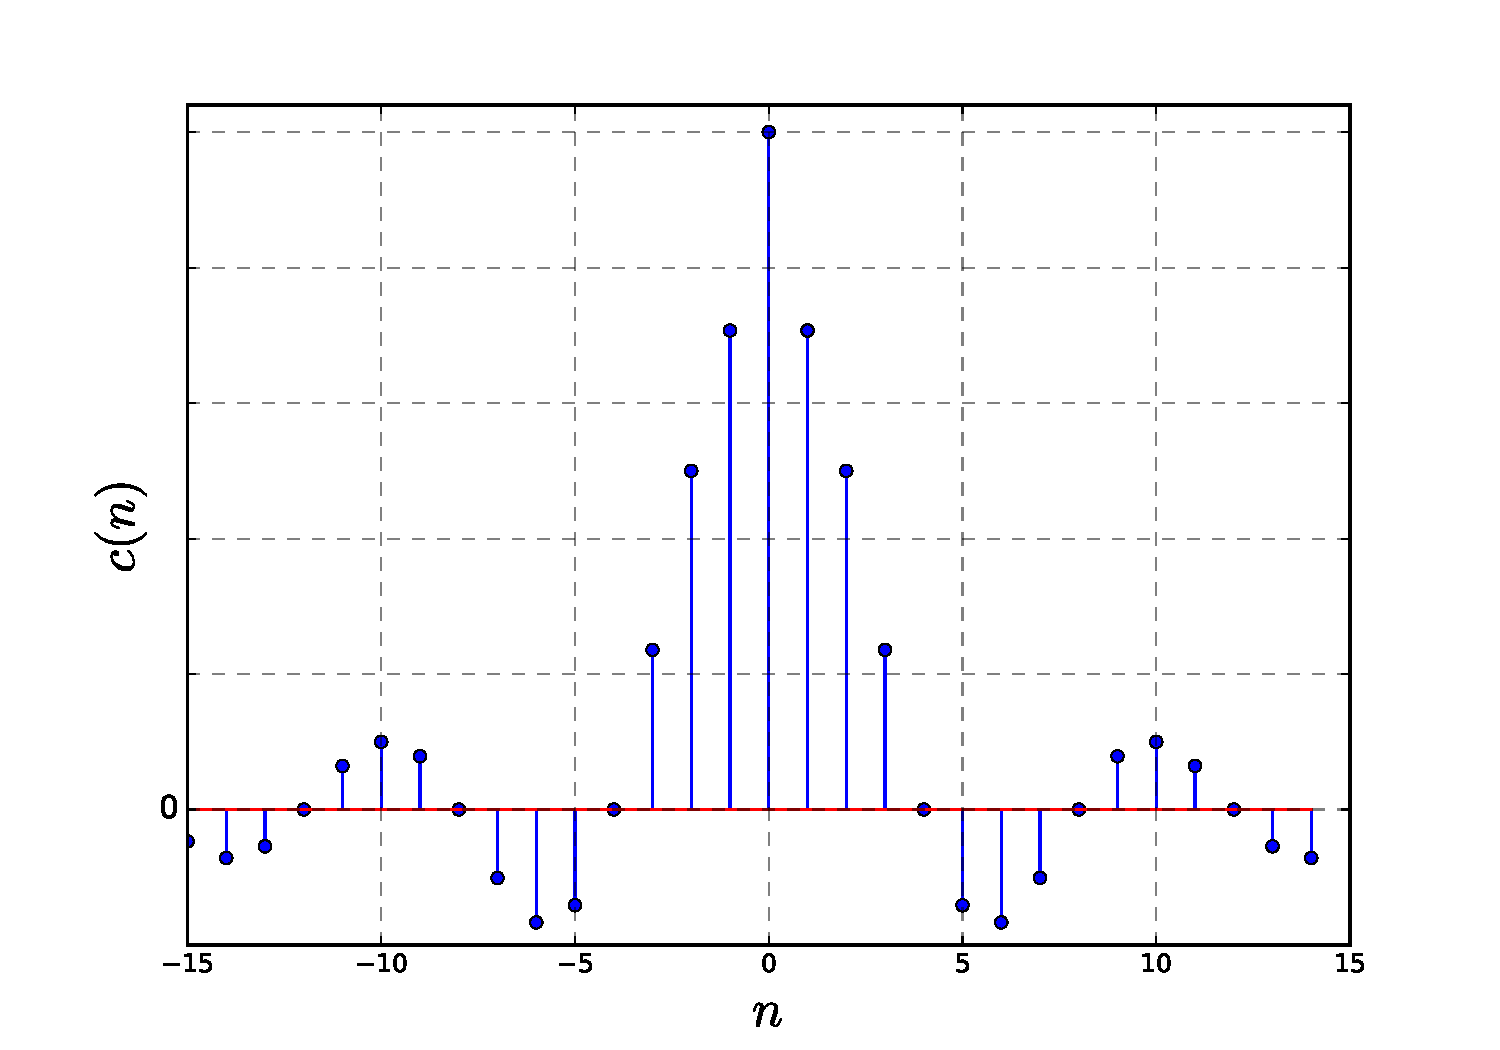
\includegraphics[scale = 0.4]{Figuras/Espectro1.pdf}
    \caption{Espectro de Fourier.}
\end{figure}

En lugar de graficar $c$ vs $n$, podemos graficar $c$ vs ``el número de onda" (frecuencia asociada a la parte espacial):
$$k = \frac{2\pi n}{L}.$$

Si $L \to \infty$, entonces las frecuencias se encuentran estrechamente espaciadas debido a que la diferencia entre valores consecutivos de $k$ es
$$\Delta k = \frac{ 2\pi \Delta n}{L}  = \frac{2\pi}{L}, \quad \mbox{pues}~ \Delta n = 1.$$

En otras palabras, para $L \to \infty$, $\Delta k$ es pequeño. Con este cambio de escala, el espectro de Fourier puede parecerse a lo mostrado en la figura \ref{Espectro1}.

\begin{figure}
    \centering
    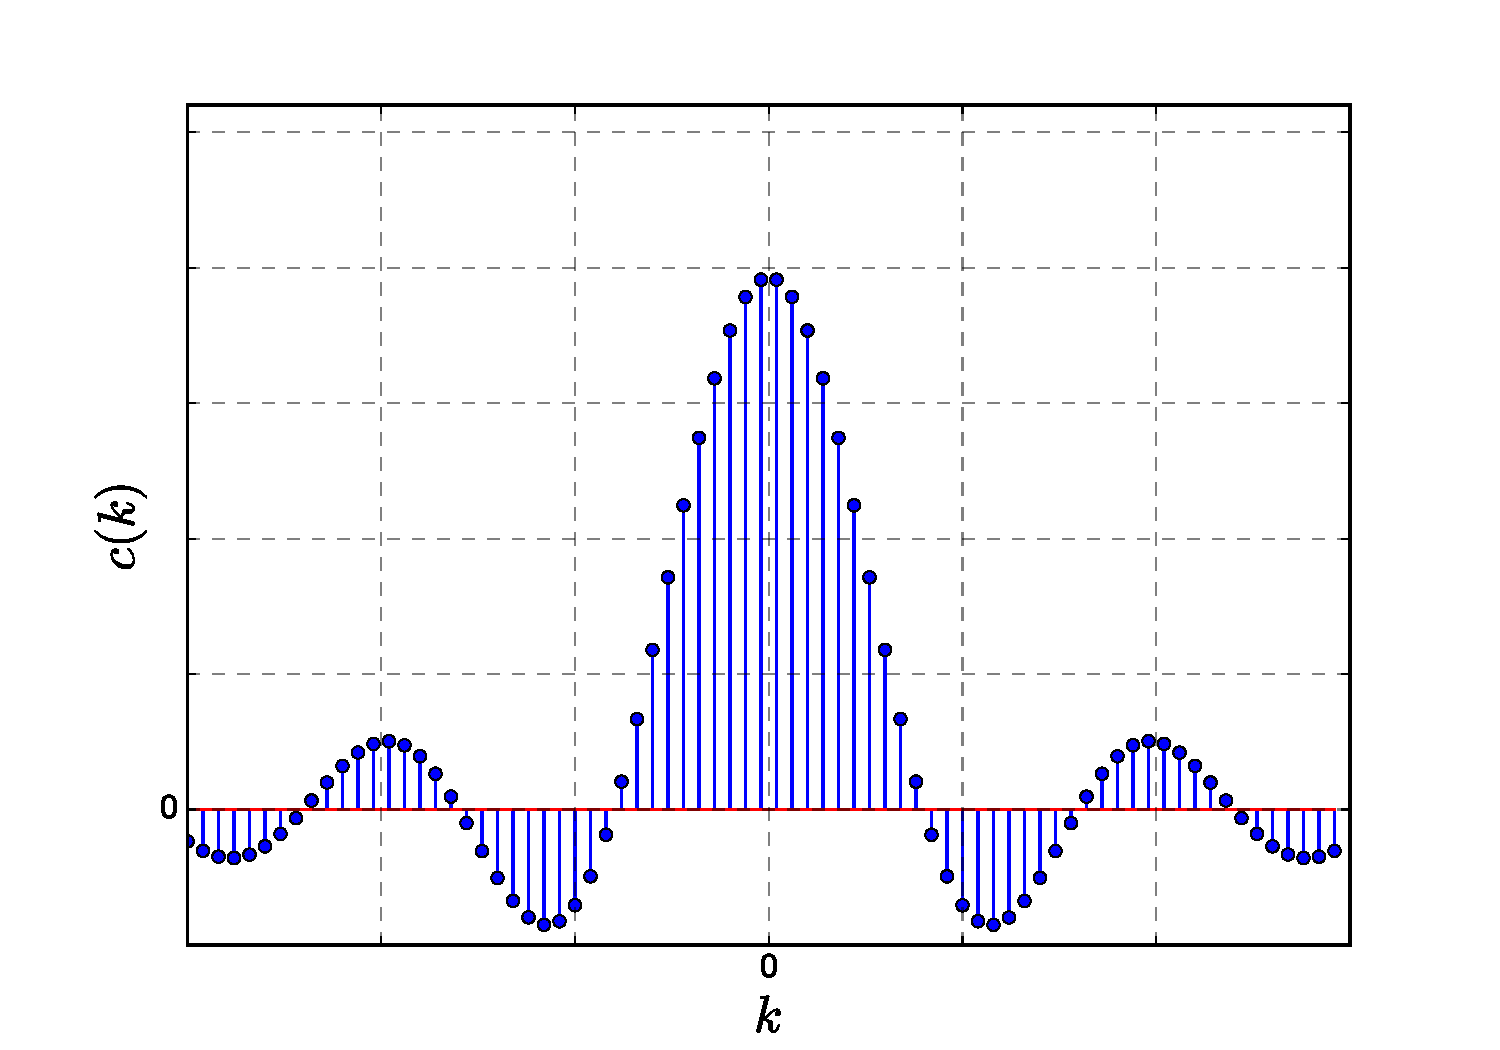
\includegraphics[scale = 0.4]{Figuras/Espectro2.pdf}    \caption{Espectro de Fourier cuando $L \to + \infty$.}
    \label{Espectro1}
\end{figure}

Es natural especular sobre la posibilidad de un espectro continuo cuando $L$ tiende al infinito  de tal forma que todas las frecuencias están presentes. Puede ser instructivo considerar la siguiente derivación heurística: Sabemos que una función puede ser expandida como una serie de Fourier tal como se muestra en \eqref{Transformada1}. Luego, la transición $L \to \infty$ puede resultar difícil de realizar directamente ya que $c_n$ aparentemente tiende a cero. Seguimos entonces la idea de usar las frecuencias $k = 2\pi n/L$ tal que
$\Delta k = (2\pi/L ) \Delta n = 2\pi/L$ para valores de $k$ adyacentes y definimos
$$c_L(k) = \frac{L}{2 \pi} c_n.$$

Usando las definiciones anteriores en las ecuaciones \eqref{Transformada1} y \eqref{Transformada2}, obtenemos: 
\begin{align*}
    f(x)&= \sum_{Lk/2\pi = -\infty}^{\infty} \frac{2\pi}{L} c_L(k) e^{ikx} \left( \frac{\Delta k L}{2\pi}\right) = \sum_{Lk/2\pi = -\infty}^{\infty}  c_L(k) e^{ikx} \Delta k , \\
  c_L(k) &= \frac{L}{2\pi} \frac{1}{L} \int_{-L/2}^{L/2} f(x) e^{-ikx} dx = \frac{1}{2\pi} \int_{-L/2}^{L/2} f(x) e^{-ikx} dx.
\end{align*}

Al hacer $L \to \infty$, la función $f$ puede considerarse como una
función no-periódica arbitraria definida en todo el intervalo $(-\infty, \infty)$ y  esperamos que la primera suma ``pase"  \text{a} una integral:
\begin{align*}
    f(x)&= \int_{-\infty}^{\infty} c(k) e^{ikx} \,dk, \\
  c(k) &= \lim_{L\to + \infty} c_L(k) =  \frac{1}{2\pi}  \int_{-\infty}^{\infty} f(x) e^{-ikx} dx.
\end{align*}

De aquí, definimos la \textbf{transformada de Fourier} de la función $f(x)$ como 
\begin{shaded}
  \begin{equation}
 \tilde{f}(k) := \frac{1}{2\pi} \int_{-\infty}^{\infty} f(x) e^{-ikx} dx \label{T.Fourier},
\end{equation}  
\end{shaded}

de modo que la ``transformada inversa" \, \text{resulta} ser
\begin{shaded}
  \begin{equation}
 f(x) =  \int_{-\infty}^{\infty} \tilde{f}(k) e^{ikx} \,dk. \label{I.Fourier}
\end{equation}  
\end{shaded}

 Note que la transformada de Fourier es la extensión natural del concepto de series de Fourier para funciones no periódicas. Además, al ser $n$ una variable discreta, y $k$ continua, podemos decir que la transformada de Fourier es la generalización del concepto de series de Fourier cuando las funciones pertenecen a un espacio vectorial de dimensión continua.

\textbf{Observaciones:}
\begin{itemize}
    \item Otras notaciones usadas son: $\tilde{f}(k) = g(k) = \mathcal{F}\{f(x)\}(k)$.
    
    \item El factor $1/2\pi$ en la definición \eqref{T.Fourier} es hasta cierto punto convencional. Lo importante es que se cumpla la identidad
    \begin{equation}
        f(x) = \int_{-\infty}^{\infty} \left[\frac{1}{2\pi} \int_{-\infty}^{\infty} f(\xi) e^{-ik\xi} d\xi \right] e^{ikx} \,dk.
      \label{IntegralFourier}
    \end{equation}
   
    Por ejemplo, en lugar de estos factores, podría introducirse un $\alpha$ en \eqref{I.Fourier} y $1/(2\pi \alpha)$ en \eqref{T.Fourier}, con $\alpha$ una constante arbitraria. Algunas elecciones populares son: $\alpha = 1$ y $\alpha = 1/\sqrt{2\pi}$ \cite{Rubilar}.

    \item Al igual que el factor $1/2\pi$ en la definición \eqref{T.Fourier}, la función $e^{-ikx}$ es convencional y puede ser reemplazada por $e^{ikx}$, siempre y cuando se verifique \eqref{IntegralFourier} \cite{Butkov, Riley}.
    
    \item En el caso que $f(x)$ sea real, tenemos que \eqref{IntegralFourier} se puede escribir como 
    \begin{equation}
        f(x) = \frac{1}{\pi} \int_{0}^{\infty} \int_{-\infty}^{\infty} f(\xi) \cos k(x-\xi)  \, d\xi \,dk.  \label{IntegralFourierReal}
    \end{equation}

    \colorlet{shadecolor}{blue!10} 
    \begin{shaded}
    En efecto, la relación \eqref{IntegralFourier} también se puede expresar como 
    $$f(x) = \frac{1}{2\pi}  \int_{-\infty}^{\infty} \int_{-\infty}^{\infty} f(\xi) e^{-ik\xi} e^{ikx} d\xi  \,dk = \frac{1}{2\pi}  \int_{-\infty}^{\infty} \int_{-\infty}^{\infty} f(\xi) e^{ik(x-\xi)} d\xi  \,dk.$$
    
    Como $f(x)$ es real, se igualan las partes reales para así obtener
    $$f(x) = \frac{1}{2\pi} \int_{-\infty}^{\infty} \int_{-\infty}^{\infty} f(\xi) \cos k(x-\xi) d\xi  \,dk. $$
    
    Puesto que $\cos k(x-\xi)$ es par con respecto a $k$, tenemos que 
    $$f(x) = \frac{2}{2\pi} \int_{0}^{\infty} \int_{-\infty}^{\infty} f(\xi) \cos k(x-\xi)  \, d\xi \,dk =\frac{1}{\pi} \int_{0}^{\infty} \int_{-\infty}^{\infty} f(\xi) \cos k(x-\xi)  \, d\xi \,dk. $$  
    \end{shaded}
    \colorlet{shadecolor}{green!20}
    
    \item Es común en Física trabajar con funciones del tiempo, $f = f(t)$. En este caso, se acostumbra usar la frecuencia $\omega$ en lugar del número de onda $k$, de modo que la integral de Fourier adopta a forma
    $$
    f(t) = \int_{- \infty}^{\infty} \Tilde{f}(\omega) e^{i \omega t} d\omega,
    $$

    donde
    $$
    \Tilde{f}(\omega) = \frac{1}{2\pi} \int_{- \infty}^{\infty} f(t) e^{- i \omega t} dt.
    $$
    
    \item En 3 dimensiones, la integral de Fourier está dada por:
    \begin{align*}
         f(\vec{r}\,) &:= \int_{\mathbb{R}^3} \tilde{f}(\vec{k}) e^{i (\vec{k} \cdot \vec{r})} d^3k, \\
         \tilde{f}(\vec{k}\,) &:= \frac{1}{(2\pi)^3} \int_{\mathbb{R}^3} f(\vec{r}) e^{-i (\vec{k} \cdot \vec{r})} d^3x.
    \end{align*}
    
    En general, en $n$ dimensiones:
     \begin{align*}
         f(\vec{r}\,) &:= \int_{\mathbb{R}^n} \tilde{f}(\vec{k}) e^{i (\vec{k} \cdot \vec{r})} d^n k, \\
         \tilde{f}(\vec{k}\,) &:= \frac{1}{(2\pi)^n} \int_{\mathbb{R}^n} f(\vec{r}) e^{-i (\vec{k} \cdot \vec{r})} d^n x.
    \end{align*}
   
\end{itemize}


\begin{defi}
Si $f(x)$ es tal que 
$$\int_{-\infty}^{\infty} |f(x)| \,dx < \infty,$$

entonces se dice que $f \in  L^1$ o que es \textbf{absolutamente integrable}.
\end{defi}

\begin{teorema}
Si $f \in L^1$, entonces la transformada de Fourier $\tilde{f}(k) = \mathcal{F}\{f(x)\}(k)$ existe y $\lim\limits_{k \to \pm \infty} \tilde{f}(k) = 0$.
\end{teorema}

\begin{demo}

Demostraremos solo la primera parte del teorema.

Notemos que
$$e^{-ikx} = \cos(kx) - i \sin(kx) ~\Rightarrow~ |e^{-ikx}| = 1.$$

Luego,
$$ \int_{-\infty}^{\infty} |f(x) e^{-ikx}| dx =  \int_{- \infty}^{\infty} |f(x)| \,dx < \infty.$$

En consecuencia, $f(x) e^{-ikx}$ es absolutamente integral y
$$\frac{1}{2\pi} \int_{-\infty}^{\infty} f(x) e^{-ikx} dx$$

es finita, es decir, $\tilde{f}(k)$ existe. 
\end{demo}

\textbf{Observación:} La condición de que $f$ sea absolutamente integrable es suficiente pero no necesaria para la existencia de la transformada de Fourier.

\begin{teorema}
    Sea $f(x)$ una función seccionalmente continua en cada intervalo finito del eje $x$, y supongamos que es absolutamente integrable en $(-\infty, + \infty)$. Entonces la \textbf{integral de Fourier}
$$
\frac{1}{\pi} \int_0^{+\infty} \int_{-\infty}^{+\infty} f(\xi) \cos k(\xi-x) \,d\xi dk = \frac{f(x^+) + f(x^-)}{2},
$$

donde ambas derivadas laterales, $f'(x^+)$ y $f'(x^-)$, existen.
\end{teorema}

\begin{demo}
Consulte el cápitulo 6 <<Fourier Integrals and Applications>> en \cite{Brown}.
\end{demo}

\section{Ejemplos}

\begin{ejemplo}[Pulso cuadrado] \label{PulsoCuadrado}
Consideremos la función 
$$f(x) = \left\{ \begin{array}{cl}
     1,& |x|<a  \\
     0,& |x|> a
\end{array} \right..$$

Su transformada de Fourier es 
\begin{align}
    \tilde{f}(k) = \frac{1}{2\pi} \int_{-\infty}^{\infty} f(x) e^{-ikx} dx &= \frac{1}{2\pi}\int_{-a}^a (1)  e^{-ikx} dx \nonumber \\
    &= \frac{1}{2\pi} \left[ - \frac{1}{ik} e^{-ikx} \right]_{-a}^a \nonumber\\
    &= \frac{1}{2\pi i k} [e^{ika} - e^{-ika}] \nonumber\\
    &= \frac{\sin(ka)}{\pi k}. \label{TransPulsoCuadrado}
\end{align}

\begin{figure}[H]
    \centering
    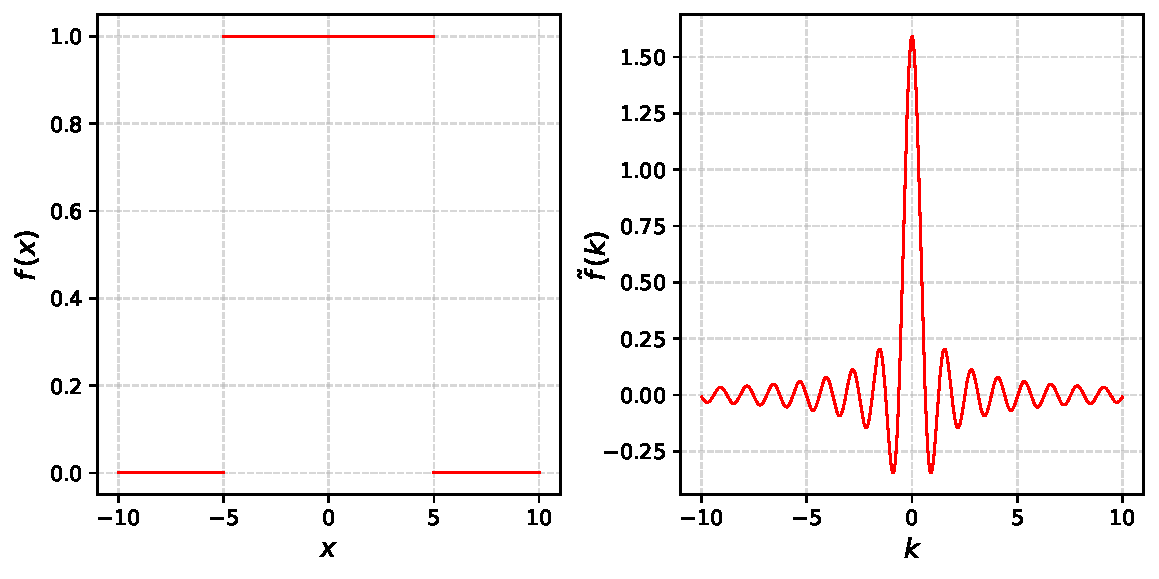
\includegraphics[scale = 0.55]{Figuras/EjemploTransformada1.pdf}
    \caption{Pulso cuadrado y su transformada de Fourier, con $a = 5$.}
    \label{Espectro2}
\end{figure}

\end{ejemplo}

\begin{ejemplo}[Distribución gaussiana]

Considere la gaussiana
$$f(x) = n e^{-\alpha x^2}, \quad  \alpha > 0.$$

Su transformada de Fourier está dada por 
\begin{equation*}
    \tilde{f}(k) =  \frac{n}{2\pi} \int_{-\infty}^{\infty} e^{-\alpha x^2} e^{-ikx} dx =  \frac{n}{2\pi} \int_{-\infty}^{\infty} e^{-\alpha x^2-ikx} dx .
\end{equation*}

Notemos que 
\begin{align*}
    -\alpha x^2-ikx &= - \alpha \left( x^2 + \frac{ik}{\alpha}x \right) \\
    &= - \alpha \left( x^2 + \frac{ik}{\alpha} x + \left( \frac{ik}{2\alpha} \right)^2 - \left( \frac{ik}{2\alpha} \right)^2 \right) \\
    &= - \alpha \left( x + \frac{ik}{2\alpha} \right)^2 + \alpha \left( \frac{ik}{2\alpha} \right)^2 \\
    &= - \alpha \left( x + \frac{ik}{2\alpha} \right)^2 - \left( \frac{k^2}{4\alpha} \right).
\end{align*}

Luego, 
\begin{equation*}
    \tilde{f}(k) =  \frac{n}{2\pi} \int_{-\infty}^{\infty} e^{-\alpha \left( x + \frac{ik}{2\alpha} \right)^2 - \left( \frac{k^2}{4\alpha} \right)}  dx = \frac{n}{2\pi} e^{- \left( \frac{k^2}{4\alpha} \right)} \int_{-\infty}^{\infty} e^{-\alpha \left( x + \frac{ik}{2\alpha} \right)^2} \,dx. 
\end{equation*}

Probaremos, usando las herramientas que nos brinda el Cálculo Complejo, que
$$
 \int_{-\infty}^{\infty} e^{-\alpha \left( x + \frac{ik}{2\alpha} \right)^2} \,dx =  \int_{-\infty}^{\infty} e^{- \alpha x^2} dx.
$$

Consideremos la integral 
\begin{equation}
   \int_{\gamma} e^{-\alpha \left( z + \frac{ik}{2\alpha} \right)^2} dz \label{IntegralComplexGauss} 
\end{equation}

donde el contorno $\gamma$ es un rectángulo que está ilustrado en la figura \ref{fig:ContornoGauss}.

\begin{figure}[H]
    \centering
    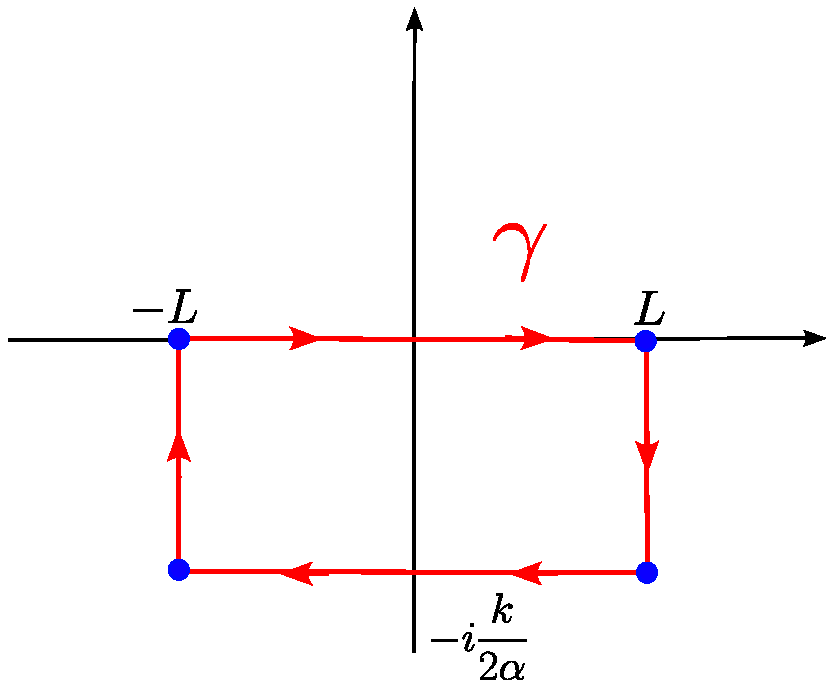
\includegraphics[scale = 0.53]{Figuras/ContornoFourierGauss.pdf}
    \caption{Contorno cerrado orientado positivamente, $\gamma$, constituido por la unión del segmento dirigido de $-L$ a $L$, de $L$ a $L - ik/2\alpha$, de $L - ik/2\alpha$ a $-L - ik/2\alpha$ y de $-L - ik/2\alpha$ a $-L$.}
    \label{fig:ContornoGauss}
\end{figure}

Como el integrando no tiene singularidades dentro del rectángulo, entonces por el teorema de Cauchy-Goursat, la integral \eqref{IntegralComplexGauss} es igual a cero. Así, evaluando la integral en cada segmento,
\begin{align*}
 \int_{\gamma} e^{-\alpha \left( z + \frac{ik}{2\alpha} \right)^2} dz &= \int_{-L}^L e^{-\alpha \left( x + \frac{ik}{2\alpha} \right)^2} dx + \int_0^{- \frac{k}{2\alpha}} i e^{-\alpha \left( L + i \left( y + \frac{k}{2\alpha} \right) \right)^2} dy   \\
 & \quad - \int_{-L}^L e^{-\alpha x^2} dx + \int_{- \frac{k}{2\alpha}}^0 i e^{-\alpha \left(- L + i \left( y + \frac{k}{2\alpha} \right) \right)^2} dy = 0.
\end{align*}

La segunda y cuarta integral, al lado derecho de la igualdad, se anulan cuando $L \to + \infty$. Luego,
$$\lim_{L \to + \infty} \int_{-L}^L e^{-\alpha \left( x + \frac{ik}{2\alpha} \right)^2} dx = \lim_{L \to + \infty} \int_{-L}^L e^{-\alpha x^2} dx.$$

Pero, las integrales
$$\int_{- \infty}^{\infty} e^{-\alpha \left( x + \frac{ik}{2\alpha} \right)^2} dx ~~\mbox{y}~~ \int_{-\infty}^{\infty} e^{-\alpha x^2} dx$$

convergen (¿Por qué?), entonces sus valores coinciden con su valor principal de Cauchy. Por lo tanto,
$$\int_{-\infty}^{\infty} e^{-\alpha \left( x + \frac{ik}{2\alpha} \right)^2} \,dx = \lim_{L \to + \infty} \int_{-L}^L e^{-\alpha \left( x + \frac{ik}{2\alpha} \right)^2} dx = \lim_{L \to + \infty} \int_{-L}^L e^{-\alpha x^2} dx = \int_{-\infty}^{\infty} e^{-\alpha x^2} \,dx.$$

Volviendo al cálculo de la transformada de Fourier,
$$
\Tilde{f}(k) = \frac{n}{2\pi} e^{- \left( \frac{k^2}{4\alpha} \right)} \int_{-\infty}^{\infty} e^{-\alpha x^2} \,dx.
$$

Como
$$\int_{-\infty}^{\infty} e^{-\alpha x^2} \,dx = \sqrt{\frac{\pi}{\alpha}}, \quad \alpha > 0$$

obtenemos que 
$$\tilde{f}(k) = \frac{n}{2\pi}\sqrt{\frac{\pi}{\alpha}}e^{- \left( \frac{k^2}{4\alpha} \right)}.$$

\begin{figure}[H]
    \centering
    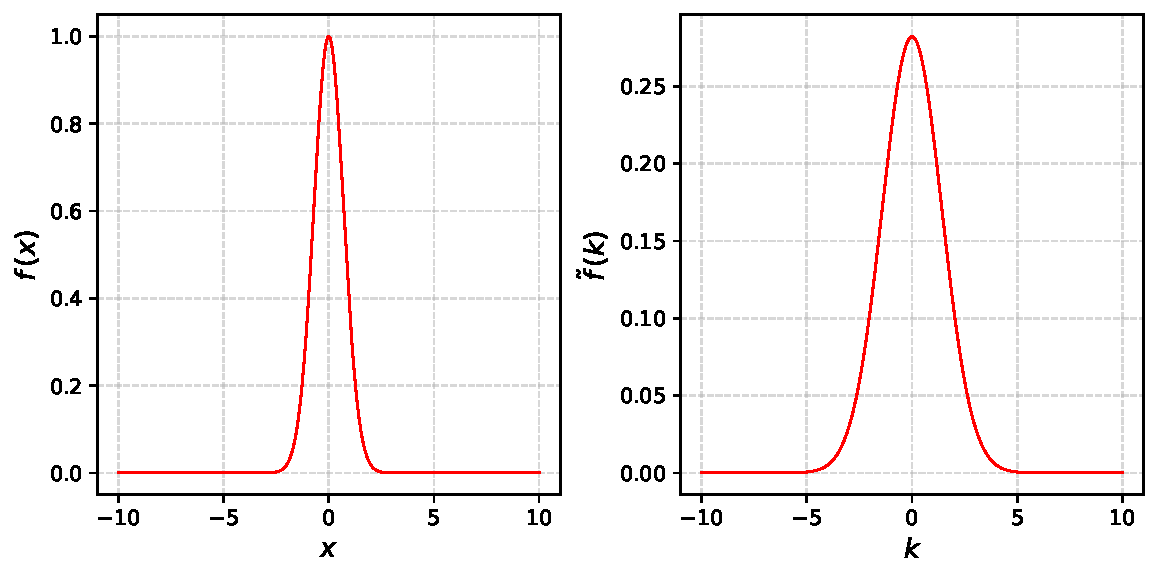
\includegraphics[scale = 0.6]{Figuras/EjemploTransformada2.pdf}
    \caption{Distribución gaussiana y su transformada de Fourier para $n=1$ y $\alpha =1$ .}
    \label{Espectro3}
\end{figure}

\begin{figure}[H]
    \centering
    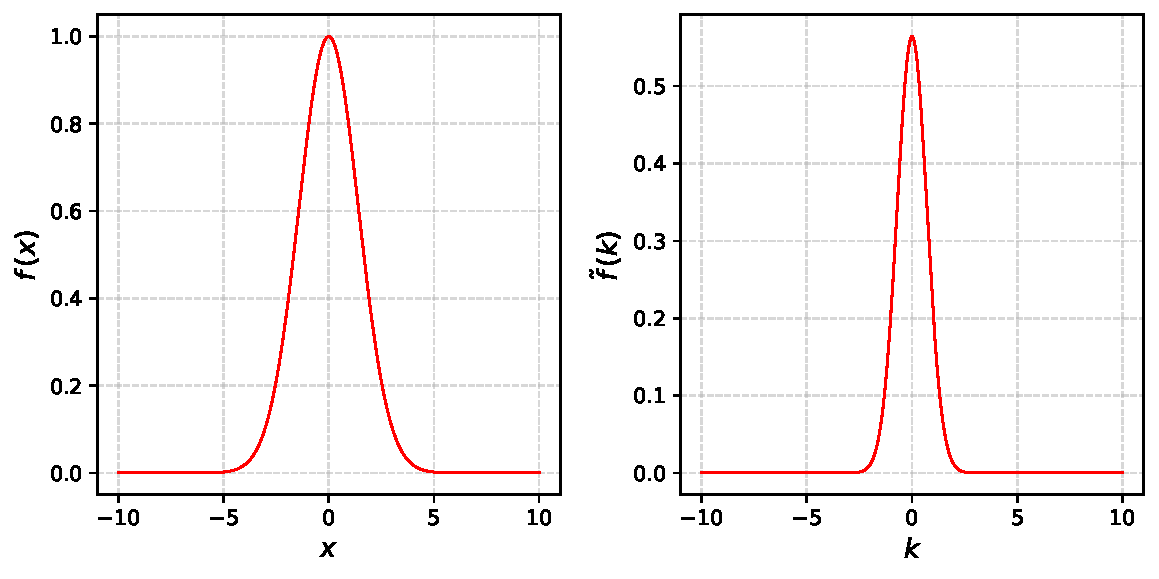
\includegraphics[scale = 0.6]{Figuras/EjemploTransformada3.pdf}
    \caption{Distribución gaussiana y su transformada de Fourier para $n=1$ y $\alpha =0.25$ .}
    \label{Espectro4}
\end{figure}
\end{ejemplo}

\begin{ejemplo}[Paridad]
Si $f(x) \in \mathbb{R}$ e impar, entonces
\begin{align*}
     \tilde{f}(k) &= \frac{1}{2\pi} \int_{-\infty}^{\infty} f(x) e^{-ikx} dx \\
&= \frac{1}{2\pi} \int_{-\infty}^0 f(x) e^{-ikx} \,dx + \frac{1}{2\pi} \int_{0}^{\infty} f(x) e^{-ikx} \, dx  \\
 &= -\frac{1}{2\pi} \int_{\infty}^0 f(-x) e^{ikx} \,dx + \frac{1}{2\pi} \int_{0}^{\infty} f(x) e^{-ikx} \, dx \\
     &= -\frac{1}{2\pi} \int_{0}^{\infty} f(x) e^{ikx} \,dx + \frac{1}{2\pi} \int_{0}^{\infty} f(x) e^{-ikx} \, dx  \\
      &= -\frac{1}{2\pi} \int_{0}^{\infty} f(x) [e^{ikx} - e^{-ikx}  ] \,dx \\
     &= -\frac{2i}{2\pi} \int_{0}^{\infty} f(x) \sin(kx) \,dx \equiv - i  \tilde{f}_S(k),
     \end{align*}
     
     donde $\tilde{f}_S$ es conocida como la \textbf{transformada seno de Fourier} de la función $f(x)$, y viene definida por 
     $$\boxed{\tilde{f}_S(k) = \frac{1}{\pi}  \int_{0}^{\infty} f(x) \sin(kx) \,dx}$$
     
Análogamente a la definición de la  transformada seno de Fourier, si $f(x) \in \mathbb{R}$ y par, entonces 
\begin{align*}
     \tilde{f}(k) = \frac{1}{2\pi} \int_{-\infty}^{\infty} f(x) e^{-ikx} dx &= \frac{1}{2\pi} \int_{-\infty}^0 f(x) e^{-ikx} \,dx + \frac{1}{2\pi} \int_{0}^{\infty} f(x) e^{-ikx} \, dx  \\
     &= -\frac{1}{2\pi} \int_{\infty}^0 f(-x) e^{ikx} \,dx + \frac{1}{2\pi} \int_{0}^{\infty} f(x) e^{-ikx} \, dx \\
     &= \frac{1}{2\pi} \int_{0}^{\infty} f(x) e^{ikx} \,dx + \frac{1}{2\pi} \int_{0}^{\infty} f(x) e^{-ikx} \, dx \\
     &= \frac{1}{2\pi} \int_{0}^{\infty} f(x) [e^{ikx} + e^{-ikx}  ] \,dx \\
     &= \frac{2}{2\pi} \int_{0}^{\infty} f(x) \cos(kx) \,dx \equiv  \tilde{f}_C(k),
     \end{align*}
     
donde $\tilde{f}_C$ es conocida como la \textbf{transformada coseno de Fourier} de la función $f(x)$, y viene definida por 
     $$\boxed{\tilde{f}_S(k) = \frac{1}{\pi}  \int_{0}^{\infty} f(x) \cos(kx) \,dx}$$

\textbf{Observación: } Esta forma de escribir la transformada seno y coseno de Fourier es convencional, por el factor $1/\pi$ y fueron adaptadas de \cite{Arfken} de tal forma que se siga la convención de este apunte.
\end{ejemplo}

\begin{comment}
\begin{ejemplo}
Consideremos ahora una función $f(x) \notin L^1$. Sea $f(x) = \sign(x)$  tal que $f(x) \notin L^1$, ya que $\int\limits_{-\infty}^{\infty}  |f(x)| \,dx$ diverge. Intentemos de todas maneras evaluar la transformada de Fourier, teniendo en cuenta que $f$ es real e impar.

\begin{align*}
    \tilde{f}(k) = \frac{1}{2\pi} \int_{-\infty}^{\infty} \sign(x) e^{-ikx} \,dx &= -\frac{i}{\pi} ^*\int_{0}^{\infty} \sin kx \,dx \qquad \mbox{(Integral de Cesàro)} \\
    &= \left\{ \begin{array}{cl}
        \frac{1}{i \pi k},  & k \neq 0  \\
         0, & k = 0
    \end{array} \right. .
\end{align*}

\end{ejemplo}    
\end{comment}

\section{Propiedades de la transformada de Fourier}

\begin{propo}
Sean $f, g \in L^1$ y $\alpha, \beta \in \mathbb{C}.$

\begin{enumerate}
    \item \textbf{Linealidad}: $$\mathcal{F}\{\alpha f(x) + \beta g(x)\}(k) = \alpha \mathcal{F}\{f(x)\}(k) + \beta \mathcal{F}\{g(x)\}(k).$$ 
    
    \item Si $f$ es real, entonces $$ \mathcal{F}\{f(x)\}(-k) = (\mathcal{F}\{f(x)\}(k))^*.$$
    
    \item \textbf{Desplazamiento}: $$\mathcal{F}\{f(x+a)\}(k) = e^{ika} \mathcal{F}\{f(x)\}(k), \quad a \in \mathbb{R}.$$
    
    \item  \textbf{Atenuación}: $$\mathcal{F}\{f(x)e^{-ax}\}(k) =  \mathcal{F}\{f(x)\}(k-ia), \quad a \in \mathbb{C}.$$
\end{enumerate}
\end{propo}

\begin{demo}
\

\begin{enumerate}
    \item Por la definición \eqref{T.Fourier} de la transformada de Fourier y usando el hecho de que las funciones son absolutamente convergentes, tenemos
    \begin{align*}
        \mathcal{F}\{\alpha f(x) + \beta g(x)\}(k) &= \frac{1}{2\pi} \int_{-\infty}^{\infty} [\alpha f(x) + \beta g(x)] e^{-ikx} dx \\
        &= \frac{\alpha}{2\pi} \int_{-\infty}^{\infty}  f(x) e^{-ikx} dx + \frac{\beta}{2\pi} \int_{-\infty}^{\infty}  g(x) e^{-ikx} dx \\
        &= \alpha \mathcal{F}\{f(x)\}(k) + \beta \mathcal{F}\{g(x)\}(k).
    \end{align*}
    
    \item Por la definición \eqref{T.Fourier} de la transformada de Fourier y suponiendo que $f$ es real:
    \begin{align*}
        \mathcal{F}\{f(x)\}(-k) &= \frac{1}{2\pi} \int_{-\infty}^{\infty}  f(x)  e^{-(-ikx)} dx  \\
        &= \frac{1}{2\pi} \int_{-\infty}^{\infty}  f(x)  (e^{-ikx})^* dx  \\
        &= \frac{1}{2\pi} \int_{-\infty}^{\infty}  [f(x)  e^{-ikx}]^* dx \\
        &= (\mathcal{F}\{f(x)\}(k))^*.
    \end{align*}
    
    \item Por la definición \eqref{T.Fourier} de la transformada de Fourier, se tiene que
$$\mathcal{F}\{f(x+a)\}(k) = \frac{1}{2\pi} \int_{-\infty}^{\infty} f(x+a) e^{-ikx} dx. $$

Haciendo la sustitución $s = x +a ~\Rightarrow~ ds = dx$:
\begin{eqnarray*}
 \frac{1}{2\pi} \int_{-\infty}^{\infty} f(x+a) e^{-ikx} dx &=& \frac{1}{2\pi} \int_{-\infty}^{\infty} f(s) e^{-ik(s-a)} \,ds \\
 &=& \frac{1}{2\pi} \int_{-\infty}^{\infty} f(s) e^{-iks+ika} \,ds \\
&=& \frac{1}{2\pi} \int_{-\infty}^{\infty} f(s) e^{-iks} e^{ika} \,ds \\
&=& e^{ika}  \left(\frac{1}{2\pi} \int_{-\infty}^{\infty} f(s) e^{-iks} \,ds \right) \\
&=& e^{ika} \mathcal{F}\{f(x)\}(k).
\end{eqnarray*}

\item Por la definición \eqref{T.Fourier} de la transformada de Fourier, tenemos que
\begin{eqnarray*}
\mathcal{F}\{f(x) e^{-ax}\}(k) &=& \frac{1}{2\pi} \int_{-\infty}^{\infty} f(x) e^{-ax} e^{-ikx} dx \\
&=& \frac{1}{2\pi} \int_{-\infty}^{\infty} f(x) e^{-ikx-ax} dx \\
&=& \frac{1}{2\pi} \int_{-\infty}^{\infty} f(x) e^{-ikx+i^{2}ax} dx \\
&=& \frac{1}{2\pi} \int_{-\infty}^{\infty} f(x) e^{-ix(k-ia)} dx \\
&=&  \mathcal{F}\{f(x)\}(k-ia).
\end{eqnarray*}

\item Usando la definición \eqref{T.Fourier} de la transformada de Fourier, obtenemos que 
\begin{equation}
  \mathcal{F}\{f(\alpha x)\}(k) = \frac{1}{2\pi} \int_{-\infty}^{\infty} f(\alpha x) e^{-ikx} dx.   \label{PropiedadTransformada}
\end{equation}

Supongamos que $\alpha > 0$, entonces hacemos el cambio de variable $u = \alpha x ~\Rightarrow~ du = \alpha dx$, para así obtener
\begin{align*}
     \frac{1}{2\pi} \int_{-\infty}^{\infty} f(\alpha x) e^{-ikx} dx &= \frac{1}{\alpha} \left( \frac{1}{2\pi} \int_{-\infty}^{\infty} f(u) e^{-i(k/\alpha)u} \,du \right) \\
     &= \frac{1}{\alpha} \mathcal{F}\{f(x)\} \left(\frac{k}{\alpha} \right).
\end{align*}

Ahora, si $\alpha < 0$, hacemos el mismo cambio de variable  en \eqref{PropiedadTransformada}:
\begin{align*}
     \frac{1}{2\pi} \int_{-\infty}^{\infty} f(\alpha x) e^{-ikx} dx &= \frac{1}{\alpha} \left( \frac{1}{2\pi} \int_{\infty}^{-\infty} f(u) e^{-i(k/\alpha)u} \,du \right) \\
     &= - \frac{1}{\alpha} \left( \frac{1}{2\pi} \int_{-\infty}^{\infty} f(u) e^{-i(k/\alpha)u} \,du \right) \\
     &= -\frac{1}{\alpha} \mathcal{F}\{f(x)\} \left(\frac{k}{\alpha} \right).
\end{align*}

Por lo tanto, 
$$\mathcal{F}\{f(\alpha x)\}(k) = \frac{1}{|\alpha|}\mathcal{F}\{f(x)\}\left(\frac{k}{ \alpha}\right), \quad \alpha \neq 0.$$

\end{enumerate}
\end{demo}

\begin{propo}
Sea $f(x)$ con transformada de Fourier $\mathcal{F}\{f(x)\}$ y $\lim\limits_{x \to \pm \infty} f(x) = 0$. Entonces, 
$$\boxed{\mathcal{F}\{f'(x)\} = i k \mathcal{F}\{f(x)\}}$$
\end{propo}

\begin{demo}
Usando la definición \eqref{T.Fourier} de la transformada de Fourier, tenemos que 
\begin{align*}
    \mathcal{F}\{f'(x)\} &= \frac{1}{2\pi} \int_{- \infty}^{\infty} f'(x) e^{-ikx} \,dx \\
    &= \frac{1}{2\pi} \int_{- \infty}^{\infty} \left\{ \frac{d}{dx}\left[ f(x) e^{-ikx} \right]  - (-ik) f(x) e^{-ikx} \right\}\,dx \\
    &= \frac{1}{2\pi} \left. f(x) e^{-ikx} \right|_{-\infty}^{\infty} + \frac{ik}{2\pi} \int_{- \infty}^{\infty}  f(x) e^{-ikx} \,dx \\
    &=  ik \mathcal{F}\{f(x)\} + \left. f(x) e^{-ikx} \right|_{-\infty}^{\infty}.
\end{align*}

Como  $\lim\limits_{x \to \pm \infty} f(x) = 0$, obtenemos
$$\mathcal{F}\{f'(x)\} = i k \mathcal{F}\{f(x)\}.$$
\end{demo}

En general,
\begin{shaded}
$$\mathcal{F}\{f^{(n)} (x)\} = (i k)^n \mathcal{F}\{f(x)\},$$    
\end{shaded}

siempre que todas las partes integradas se anulen cuando $x \to \pm \infty$.

\begin{teorema}[de Parseval]
Si $f(x)$ y $g(x)$ son funciones reales y si $\tilde{f}(k)$ y $\tilde{g}(k)$ son sus correspondientes transformadas de Fourier, entonces

\begin{itemize}
    \item[(i)] (Primer teorema)
    $$\int_{-\infty}^{\infty} |\tilde{f}(k)|^2\, dk = \frac{1}{2\pi} \int_{-\infty}^{\infty} |f(x)|^2 \, dx. $$
    
    \item[(ii)] (Segundo teorema)
    $$\int_{-\infty}^{\infty} \tilde{f}(k) \tilde{g}(-k) \, dk = \frac{1}{2\pi} \int_{-\infty}^{\infty} f(x) g(x) \, dx. $$
    
\end{itemize}
\end{teorema}

\begin{demo}
Notemos que (i) es consecuencia de (ii) al tomar $g(x) = f(x)$ real tal que $f^*(x) = f(x)$ y $\tilde{g}(-k) = \tilde{f}^*(k)$. Luego, nos bastará demostrar el segundo teorema de Parseval.

Usando la definición \eqref{T.Fourier}, tenemos que 
$$\tilde{g}(-k) = \frac{1}{2\pi} \int_{-\infty}^{\infty} g(x) e^{ikx} \,dx.$$

Luego, 
$$\int_{-\infty}^{\infty} \tilde{f}(k) \tilde{g}(-k) \,dk = \int_{-\infty}^{\infty} \tilde{f}(k) \,dk \int_{-\infty}^{\infty} \frac{1}{2\pi} g(x) e^{ikx} \,dx.$$

Supongamos que podemos intercambiar el orden de integración, por ejemplo, al suponer que las integrales 
$$\int_{-\infty}^{\infty} \tilde{f}(k) e^{ikx} \,dk ~~\mbox{y}~~ \int_{-\infty}^{\infty} g(x) e^{ikx} \,dx$$

son absolutamente integrables. Entonces,
$$\int_{-\infty}^{\infty} \tilde{f}(k) \tilde{g}(-k) \,dk = \frac{1}{2\pi} \int_{-\infty}^{\infty} g(x) \left(  \int_{-\infty}^{\infty}  \tilde{f}(k) e^{ikx} \,dk\right) \,dx.$$

Ahora, aplicando la transformada inversa de Fourier dada por \eqref{I.Fourier}, concluimos que
$$\int_{-\infty}^{\infty} \tilde{f}(k) \tilde{g}(-k) \,dk = \frac{1}{2\pi} \int_{-\infty}^{\infty} f(x) g(x)  \,dx.$$

\end{demo}

\begin{ejemplo}
    Use el teorema de Parseval para evaluar
    $$\int_{-\infty}^{\infty}  \frac{\sin^2(x)}{x^2} \,dx.$$

    \textbf{Solución:} Esta integral puede ser calculada usando el teorema del residuo. En nuestro caso, usaremos el primer teorema de Parseval, teniendo en cuenta el resultado de la transformada de Fourier del pulso cuadrado en el ejemplo \ref{PulsoCuadrado}. 

    Para $a = 1$ en la ecuación \eqref{TransPulsoCuadrado}, tenemos que
    $$\int_{- \infty}^{\infty} |\Tilde{f}(k)|^2 \,dk = \int_{- \infty}^{\infty} \frac{\sin^2(k)}{\pi^2 k^2}  \,dk = \frac{1}{\pi^2} \int_{-\infty}^{\infty}  \frac{\sin^2(k)}{k^2} \,dk.$$

    Por el primer teorema de Parseval,
    \begin{align*}
        \int_{- \infty}^{\infty} |\Tilde{f}(k)|^2 \,dk &= \frac{1}{2\pi} \int_{-\infty}^{\infty} |f(x)|^2 \,dx \\
        \Rightarrow \frac{1}{\pi^2} \int_{-\infty}^{\infty}  \frac{\sin^2(k)}{k^2} &= \frac{1}{2\pi} \int_{-1}^1 \,dx = \frac{1}{\pi}. 
    \end{align*}

Por lo tanto,
$$\int_{-\infty}^{\infty}  \frac{\sin^2(k)}{k^2} \,dk = \pi.$$
\end{ejemplo}

\section{Convolución}

\begin{defi}
Sean $f(x)$ y $g(x)$ dos funciones reales, se define la operación \textbf{convolución} de dos funciones $f$ y $g$ como 
\begin{equation}
 (f*g)(x) := \int_{-\infty}^{\infty} f(y) g(x-y) \,dy.   \label{Convolucion}
\end{equation}

\end{defi}

\textbf{Idea física:} Sea $f(t)$ algún ``estímulo" (fuerza en el tiempo $t$, densidad de carga en la posición $x$, etc). Sea $g(x,t) = g(x-t)$ la respuesta en $x$ a un estímulo en $t$. Si el sistema es \textit{lineal}, la respuesta total en el punto $x$ al estímulo global $\{f(t) : t \in \mathbb{R}\}$ será la "suma" de todas las contribuciones $[dt\, f(t)] g(x,t)$, que es la convolución $(f*g)(x)$. 

Por ejemplo, el potencial electrostático debido a una densidad de carga $\rho(\Vec{x})$ se puede escribir como
$$\phi(\Vec{x}) = \int_{V} \frac{\rho(\Vec{x}\,')}{|\Vec{x} - \Vec{x}\,'|} \, dV' = \rho * f(\Vec{x}),$$

donde  $f(\Vec{x}) = 1/|\Vec{x}|$.

\begin{figure}[H]
    \centering
    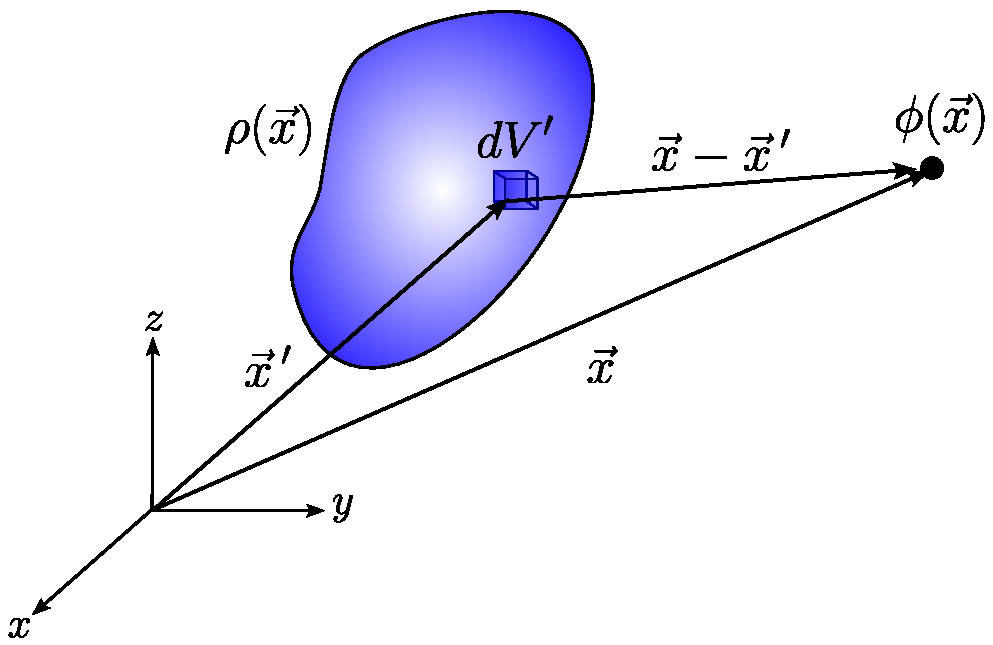
\includegraphics[scale = 0.55]{Figuras/Distribucion-Cargas.pdf}
    \caption{Distribución de carga de densidad $\rho(\Vec{x})$.}
    \label{fig:PotencialDistribucion}
\end{figure}

\textbf{Idea matemática:} La interpretación matemática de la convolución está ilustrada en la figura \ref{fig:IdeaConvolucion}.

\begin{figure}[H]
    \centering
    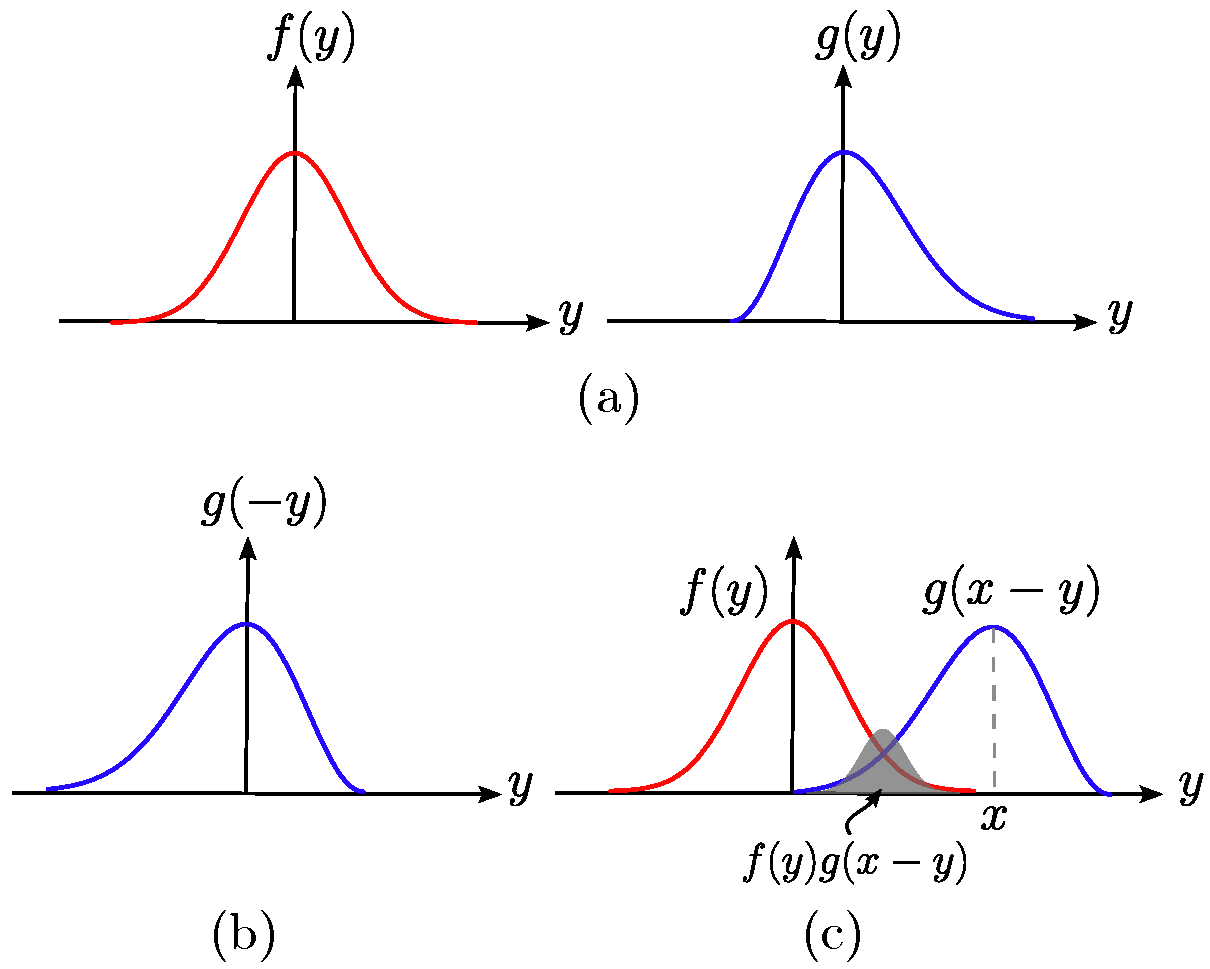
\includegraphics[scale = 0.55]{Figuras/Idea-Convolucion.pdf}
    \caption{Idea matemática de la convolución. En (a), se expresa cada función en términos de la variable de integración $y$. En (b), se refleja la gráfica de $g(y)$ con respecto al eje vertical, es decir, $g(y) \rightarrow g(-y)$. En (c), se traslada la gráfica de $g(-y)$, $x$ unidades. Luego, se traslapan las gráficas de $f(y)$ y $g(x-y)$ de tal forma que el área sombreada corresponde al valor de $f * g$ para ese valor de $x$.}
    \label{fig:IdeaConvolucion}
\end{figure}


Entonces, $f * g$ mide el grado de traslape entre $f(y)$ y $g(-y)$, luego de trasladar $g$ a una distancia $x$.

\begin{propo}[Propiedades de la convolución]
Sean $f(x)$, $g(x)$ y $h(x)$  funciones reales, se verifica:

\begin{enumerate}
    \item \textbf{Conmutatividad:}$$f(x) * g(x) = g(x) * f(x).$$
    
    \item \textbf{Asociatividad:} $$[f(x)*g(x)]*h(x) = f(x)*[g(x)*h(x)].$$
    
    \item \textbf{Distributividad:} $$f(x)*[g(x)+h(x)] = f(x)*g(x) + f(x)*h(x).$$ 
\end{enumerate}
\end{propo}

\begin{demo}
\ 

\begin{enumerate}
    \item Por \eqref{Convolucion}, se tiene
    $$(f*g)(x) =  \int_{-\infty}^{\infty} f(y) g(x-y) \,dy.$$
    
    Haciendo el cambio de variable $u = x-y ~\Rightarrow~ du = -dy$,
    $$ (f*g)(x) = - \int_{\infty}^{-\infty} f(x-u) g(u) \,du =  \int_{-\infty}^{\infty} g(u) f(x-u) \,du = (g*f)(x).$$
    
    \item Por definición:
    \begin{align}
        f(x)*[g(x)*h(x)] &=  \int_{-\infty}^{\infty} f(y) (g*h)(x-y) \,dy \nonumber\\
        &=  \int_{-\infty}^{\infty} f(y) \left( \int_{-\infty}^{\infty} g(z) h(x-y-z) \,dz \right) \,dy  \nonumber\\
        &= \int_{-\infty}^{\infty}  \left(\int_{-\infty}^{\infty}  f(y) g(z) h(x-y-z) \,dz \right) \,dy. \label{Convolucion1}
    \end{align}
    
    y
     \begin{align}
        [f(x)*g(x)]*h(x) &= \int_{-\infty}^{\infty} (f*g)(y) h(x-y) \,dy \nonumber \\
        &=  \int_{-\infty}^{\infty} h(x-y) \left( \int_{-\infty}^{\infty} f(z) g(y-z) \,dz \right) \,dy  \nonumber \\
        &=  \int_{-\infty}^{\infty}  \left(\int_{-\infty}^{\infty}  f(z) g(y-z) h(x-y) \,dz \right) \,dy \label{Convolucion2}
    \end{align}
    
    Haciendo el cambio de variable $w = y+z ~\Rightarrow~ dw = dz$ en la integral interior de \eqref{Convolucion1}, obtenemos que 
    $$ f(x)*[g(x)*h(x)] = \int_{-\infty}^{\infty} \left(\int_{-\infty}^{\infty}  f(y) g(w-y) h(x-w) dw\right) dy.$$
    
    Si el intercambio de orden de integración es posible, entonces 
      $$ f(x)*[g(x)*h(x)] =  \int_{-\infty}^{\infty} \left(\int_{-\infty}^{\infty}  f(y) g(w-y) h(x-w) dy\right) dw.$$
    
    Comparando con \eqref{Convolucion2}, concluimos que 
    $$[f(x)*g(x)]*h(x) = f(x) * [g(x) * h(x)].$$
    
    \item Por definición,
    \begin{align*}
        f(x)*[g(x)+h(x)] &=  \int_{-\infty}^{\infty} f(y) (g+h)(x-y) \,dy \\
        &= \int_{-\infty}^{\infty} f(y) [g(x-y) + h(x-y)] \,dy \\
        &=  \int_{-\infty}^{\infty} f(y)  g(x-y) \,dy +  \int_{-\infty}^{\infty}  f(y)h(x-y) \,dy \\
        &=  f(x)*g(x) + f(x)*h(x).
    \end{align*}
\end{enumerate}
\end{demo}

\begin{teorema}[de convolución de Fourier]
Sean $f(x)$, $g(x)$ y $h(x)$  funciones reales y sean $\tilde{f}(k)$, $\tilde{g}(k)$ y $\tilde{h}(k)$ sus correspondientes transformadas de Fourier. 

\begin{itemize}
    \item Si $\tilde{h}(k) = \tilde{f}(k) \tilde{g}(k)$, entonces 
$$ h(x) = \frac{1}{2\pi} (f * g)(x) = \frac{1}{2\pi} (g * f)(x) = \frac{1}{2\pi} \int_{-\infty}^{\infty} f(y) g(x-y) \,dy.$$ 

    \item Si $h(x) = f(x) g(x)$, entonces
$$\Tilde{h}(k) = (\Tilde{f} * \Tilde{g})(k) = (\Tilde{g} * \Tilde{f})(k) = \int_{-\infty}^{\infty} \Tilde{f}(y) \Tilde{g}(k-y) \,dy.$$
\end{itemize}
\end{teorema}

\begin{demo}
\ 

\begin{itemize}
    \item Supongamos que  $\tilde{h}(k) = \tilde{f}(k) \tilde{g}(k)$. Aplicando la transformada de Fourier inversa dada por \eqref{I.Fourier}, tenemos que 
\begin{align*}
   h(x) = \mathcal{F}^{-1} \{\tilde{h}(k)\} &=  \mathcal{F}^{-1} \{\tilde{f}(k) \tilde{g}(k)\} \\
   &= \int_{-\infty}^{\infty} \tilde{f}(k) \tilde{g}(k) e^{ikx} \,dk \\
   &= \frac{1}{2\pi} \int_{-\infty}^{\infty}  \left( \int_{-\infty}^{\infty} f(y) e^{-ik y} \,dy \right) \tilde{g}(k)  e^{ikx}  \,dk.
\end{align*}

Si el intercambio de orden de integración es posible, entonces 
\begin{align*}
  h(x) &= \frac{1}{2\pi} \int_{-\infty}^{\infty}  f(y)  \left( \int_{-\infty}^{\infty}  \tilde{g}(k)  e^{ikx} e^{-ik y}\,d k \right) \,dy \\
   &= \frac{1}{2\pi} \int_{-\infty}^{\infty}  f(y)  \left( \int_{-\infty}^{\infty}  \tilde{g}(k)  e^{ik(x-y)}\,d k \right) \,dy \\
   &= \frac{1}{2\pi} \int_{-\infty}^{\infty}  f(y) g(x-y) \,dy = \frac{1}{2\pi} (f * g)(x).
\end{align*}

Como la convolución es conmutativa:
$$h(x) = \frac{1}{2\pi} (f * g)(x) = \frac{1}{2\pi} (g * f)(x)  = \frac{1}{2\pi} \int_{-\infty}^{\infty}  f(y) g(x-y) \,dy.$$

\item  Supongamos que $h(x) = f(x) g(x)$. Aplicando la transformada de Fourier dada por \eqref{T.Fourier}, tenemos que 
\begin{align*}
   \Tilde{h}(k) &=  \mathcal{F} \{f(x) g(x)\} \\
   &= \frac{1}{2\pi} \int_{-\infty}^{\infty} f(x) g(x) e^{-ikx} \,dx \\
   &=  \frac{1}{2\pi} \int_{-\infty}^{\infty} \left( \int_{-\infty}^{\infty} \Tilde{f}(y) e^{iyx} \,dy \right) g(x) e^{-ikx} \,dx.
\end{align*}

Si el intercambio de orden de integración es posible, entonces 
\begin{align*}
   \Tilde{h}(k) &=  \frac{1}{2\pi} \int_{-\infty}^{\infty} \Tilde{f}(y) \left( \int_{-\infty}^{\infty} g(x) e^{iyx}  e^{-ikx}\,dx \right) \,dy \\
   &=  \int_{-\infty}^{\infty} \Tilde{f}(y) \left( \frac{1}{2\pi} \int_{-\infty}^{\infty} g(x) e^{-i(k-y)x} \,dx \right) \,dy \\
   &=  \int_{-\infty}^{\infty} \Tilde{f}(y) \Tilde{g}(k-y) \,dy. 
\end{align*}

Por lo tanto,
$$\Tilde{h}(k) =  (\Tilde{f} * \Tilde{g})(k) = (\Tilde{g} * \Tilde{f})(k) = \int_{-\infty}^{\infty} \Tilde{f}(y) \Tilde{g}(k-y) \,dy.$$
\end{itemize}

\end{demo}


\begin{ejemplo}
    Sabiendo que \cite{Mauch}
    $$\mathcal{F}\left\{ \frac{2c}{x^2+c^2} \right\} = e^{-c|k|}, \quad \text{para} ~ c > 0.$$

    Podemos usar el teorema de convolución para encontrar la transformada de Fourier de
    \begin{equation}
      f(x) = \frac{1}{x^4+5x^2+4} = \frac{1}{(x^2+1)(x^2+4)}.    \label{EjConvo}
    \end{equation}
  
    En efecto,
    \begin{align*}
        \mathcal{F}\{f(x)\} &=  \mathcal{F}\left\{ \frac{1}{8} \frac{2}{x^2+1} \frac{4}{x^2+4} \right\} \\
        &= \frac{1}{8} \left( \int_{-\infty}^{\infty} e^{-|y|}e^{-2|k-y|} dy \right) \\
        &= \frac{1}{8} \left( \int_{-\infty}^0 e^{y}e^{-2|k-y|} dy +   \int_0^{\infty} e^{-y}e^{-2|k-y|} dy \right).
    \end{align*}

Si $k > 0$,
\begin{align*}
    \mathcal{F}\{f(x)\} &= \frac{1}{8} \left(  \int_{-\infty}^0 e^{y}e^{-2(k-y)} dy +  \int_0^k e^{-y}e^{-2(k-y)} dy + \int_k^{\infty} e^{-y}e^{2(k-y)} dy \right)  \\
    &= \frac{1}{8} \left(  \int_{-\infty}^0 e^{-2k+3y} dy +  \int_0^k e^{-2k+y} dy + \int_k^{+\infty} e^{2k-3y} dy \right) \\
    &= \frac{1}{8} \left( \frac{1}{3} e^{-2k} + e^{-k} - e^{-2k} + \frac{1}{3} e^{-k} \right) \\
    &= \frac{1}{6} e^{-k} - \frac{1}{12} e^{-2k}. 
\end{align*}

Si $k < 0$,
\begin{align*}
    \mathcal{F}\{f(x)\} &= \frac{1}{8} \left(  \int_{-\infty}^k e^{y}e^{-2(k-y)} dy +  \int_k^0 e^{y}e^{2(k-y)} dy + \int_0^{\infty} e^{-y}e^{2(k-y)} dy \right)  \\
    &= \frac{1}{8} \left(  \int_{-\infty}^k e^{-2k+3y} dy +  \int_k^0 e^{2k-y} dy + \int_0^{\infty} e^{2k-3y} dy \right) \\
    &= \frac{1}{8} \left( \frac{1}{3} e^{k} - e^{2k} + e^k + \frac{1}{3} e^{2k} \right) \\
    &= \frac{1}{6} e^{k} - \frac{1}{12} e^{2k}. 
\end{align*}

Por lo tanto, para $k$ positivo como negativo,
$$\boxed{\mathcal{F}\{f(x)\} =  \frac{1}{6} e^{-|k|} - \frac{1}{12} e^{-2|k|}} $$

Una mejor forma de encontrar la transformada de Fourier de \eqref{EjConvo} es, en primer lugar, descomponer la función en fracciones parciales,
$$f(x) = \frac{1}{3} \frac{1}{x^2+1} - \frac{1}{3} \frac{1}{x^2+4},$$

para luego hacer usar de la linealidad de la transformada.
\begin{align*}
     \mathcal{F}\{ f(x)\} &= \frac{1}{6} \mathcal{F} \left\{ \frac{2}{x^2+1}\right\} - \frac{1}{12} \mathcal{F} \left\{ \frac{4}{x^2+4} \right\}  \\
     &= \frac{1}{6} e^{-|k|} - \frac{1}{12} e^{-2|k|}.
\end{align*}

\end{ejemplo}

\section{Aplicación de la transformada de Fourier}

La transformada de Fourier es útil para resolver ecuaciones diferenciales en el dominio $(-\infty, \infty)$ con condiciones de borde homogéneas en el infinito. En particular, en ecuaciones diferenciales \underline{lineales} con \underline{coeficientes constantes}, debido a la propiedad de linealidad de la transformada.

A continuación se ilustra el procedimiento a seguir mediante ejemplos.

\begin{ejemplo}
    Encuentre la solución general de la ecuación diferencial
    $$y''(x) - y(x) = e^{-\alpha |x|}, \quad y(\pm \infty) = 0, \quad \alpha > 0, \alpha \neq 1.$$

    \textbf{Solución:} La solución del caso homogéneo 
    $$y''(x) - y(x) = 0,$$

    está dada por
    $$y_h(x) = c_1 e^{x} + c_2 e^{-x}, \quad c_1,c_2 \in \mathbb{R}.$$

    Nos queda por encontrar la solución particular, para ello haremos uso de la transformada de Fourier. 

    Primero, determinemos 
    
    \begin{align*}
        \mathcal{F}\left\{ e^{-\alpha |x|} \right\} &= \frac{1}{2\pi} \int_{-\infty}^{\infty} e^{-\alpha |x|} e^{-ikx} dx \\
        &= \frac{1}{2\pi} \left(  \int_{-\infty}^{0} e^{x(\alpha -ikx)} dx +  \int_{0}^{\infty} e^{-x(\alpha + ik)} dx\right) \\
        &= \frac{1}{2\pi} \left( \frac{1}{\alpha -ik} + \frac{1}{\alpha +ik} \right) \\
        &= \frac{\alpha/\pi}{\alpha^2 + k^2}.
    \end{align*}

    Luego, apliquemos la transformada de Fourier a la ecuación diferencial:
    \begin{align*}
        \mathcal{F}\{ y''(x)\} - \mathcal{F}\{y(x)\ &=  \mathcal{F}\left\{ e^{-\alpha |x|} \right\} \\
        \Rightarrow - k^2 \mathcal{F}\{y(x)\} - \mathcal{F}\{y(x)\} &= \frac{\alpha/\pi}{\alpha^2 + k^2}.
    \end{align*}

    Despejando la transformada de Fourier de la solución.
    \begin{align*}
        \mathcal{F}\{y(x)\} &= \frac{-\alpha/\pi}{(k^2 + \alpha^2)(k^2+1)} \\
        &= - \frac{\alpha}{\pi} \frac{1}{\alpha^2-1} \left( \frac{1}{k^2+1} - \frac{1}{k^2+ \alpha^2}\right) \\
        &= \frac{1}{\alpha^2-1} \left( \frac{\alpha/\pi}{k^2 + \alpha^2} - \alpha \frac{1/\pi}{k^2+1} \right.)
    \end{align*}

    Tomando la transformada inversa, obtenemos que
    $$y(x) = \frac{e^{-\alpha|x| - \alpha e^{-|x|} }}{\alpha^2-1}.$$

    Por lo tanto, la solución general es
    $$\boxed{y(x) = \frac{e^{-\alpha|x| - \alpha e^{-|x|} }}{\alpha^2-1} + c_1 e^{x} + c_2 e^{-x}, \quad c_1,c_2 \in \mathbb{R}}$$
\end{ejemplo}

\begin{ejemplo}
  Consideremos un oscilador armónico amortiguado sometido a una fuerza externa $g(t)$. La ecuación de movimiento del oscilador está dada por
\begin{equation}
 \ddot{x}(t) + 2 \alpha \dot{x}(t) + \omega_0^2 x(t) = f(t), \label{EDO-Oscilador}   
\end{equation}

donde $f(t) = g(t)/m$ y $\alpha$ es una constante asociada al amortiguamiento del sistema. En los primeros cursos de Ecuaciones Diferenciales Ordinarias (EDO) se trabaja con $f(t)$ sinusoidal, pero gracias a la transformada de Fourier, podemos extender este resultado para funciones $f(t)$ arbitrarias. 

Aplicando la transformada de Fourier en la variable temporal, a saber,
$$\mathcal{F}\{x(t)\} = \frac{1}{2\pi} \int_{-\infty}^{\infty} f(t) e^{-i\omega t} dt, $$

a ambos lados de la ecuación diferencial \eqref{EDO-Oscilador}, obtenemos 
\begin{align}
    \mathcal{F}\left\{ \ddot{x}(t) + 2 \alpha \dot{x}(t) + \omega_0^2 x(t)\right\} &= \mathcal{F}\left\{ f(t)\right\} \nonumber\\
    \Rightarrow   \mathcal{F}\left\{ \ddot{x}(t) \right\} + 2\alpha \mathcal{F}\left\{ \dot{x}(t) \right\} + \omega_0^2 \mathcal{F}\{x(t)\} &= \mathcal{F}\left\{ f(t)\right\}. \label{EDO-Transformada}
\end{align}

Si asumimos que 
$$\lim_{x \to \pm \infty} x(t) = \lim_{x \to \pm \infty} \dot{x}(t) = 0,$$

tenemos 
\begin{align*}
     \mathcal{F}\left\{ \ddot{x}(t) \right\} &= (i\omega)^2 \mathcal{F}\{x(t)\} = - \omega^2 \mathcal{F}\{x(t)\},\\
      \mathcal{F}\left\{ \dot{x}(t) \right\} &= i \omega \mathcal{F}\{x(t)\}.
\end{align*}

Además, si definimos $F(\omega) := \mathcal{F}\left\{ f(t)\right\}$, la ecuación \eqref{EDO-Transformada} nos queda
$$ - \omega^2 \mathcal{F}\{x(t)\} + 2 \alpha \omega i \mathcal{F}\{x(t)\} + \omega_0^2 \mathcal{F}\{x(t)\} = F(\omega).$$

Despejando la transformada de Fourier de la solución:
$$  \mathcal{F}\{x(t)\} = \frac{F(\omega)}{-\omega^2 - 2 \alpha i \omega + \omega_0^2}.$$

Tomando la transformada inversa, obtenemos la solución 
$$\boxed{x(t) = \int_{-\infty}^{\infty} \frac{F(\omega)}{(\omega_0^2-\omega^2) - 2 \alpha \omega i} e^{i\omega t} d\omega }$$  
\end{ejemplo}



\chapter{Transformada de Laplace}

\section{Definición}

\begin{defi}
Sea $f(t)$ una función a valores reales definida para $t \in [0, \infty[$. La \textbf{transformada de Laplace} de $f$ es la función $F$ definida mediante la integral impropia
$$F(s) := \int_0^{\infty} e^{-st} f(t) \,dt.$$

El dominio de $F(s)$ está formado por todos lo valores de $s$ (complejos) para los que la integral existe. Simbólicamente,
$$F(s) = \mathcal{L}\{f(t)\}.$$
\end{defi}

\begin{ejemplo}
Determine la transformada de Laplace de 
$$f(t) = e^{at}.$$

\textbf{Solución:} Por definición, 
\begin{align*}
    \mathcal{L}\{e^{at}\} = \int_0^{\infty} e^{-st} e^{at} \,dt &= \int_0^{\infty} e^{-(s-a)t} \,dt \\
    &= \left. - \frac{e^{-(s-a)t}}{s-a} \right|_0^{\infty} \\
    &= \frac{1}{s-a}, \quad \real(s) > a.
\end{align*}

En efecto, si hacemos $s = \real(s) + i \im(s)$, tenemos que
$$\lim_{t\to + \infty} \left| e^{-(s-a)t} \right| = \lim_{t\to + \infty} \left|e^{-(\real(s) - a)t} \right| = 0, \quad \real(s) > a. $$
\end{ejemplo}

\begin{ejemplo}
    Consideremos la transformada de Laplace de la \textbf{función de Heaviside},
    $$H(t-a) = \left\{ \begin{array}{cl}
     0,& \text{si} ~ t < a  \\
     1,& \text{si} ~ t > a
    \end{array} \right.,$$

    para un número real $a$ no negativo.
    \begin{align*}
        \mathcal{L}\{H(t-a)\} &= \int_0^{\infty} e^{-st} H(t-a) \,dt \\
        &= \int_a^{\infty} e^{-st} \,dt \\
        &= \left. - \frac{e^{-st}}{s}\right|_a^{\infty} \\
        &= \frac{e^{-as}}{s}, \quad \real(s) > 0.
    \end{align*}

    Ahora, consideremos $H(t-a)f(t-a)$.
    \begin{align*}
        \mathcal{L}\{H(t-a)f(t-a)\} &= \int_0^{\infty} e^{-st} H(t-a)f(t-a) \,dt \\
        &= \int_a^{\infty} e^{-st} f(t-a) \,dt \\
        &= \int_0^{\infty} e^{-s(t+a)} f(t) \,dt \\
        &= e^{-as} F(s).
    \end{align*}

\end{ejemplo}

\begin{ejemplo}
    Queda como ejercicio para el lector demostrar que
    \begin{align*}
        \mathcal{L}\{\cos(at)\} &= \frac{s}{s^2+a^2}, \quad \real(s) > 0, \\
        \mathcal{L}\{\sin(at)\} &= \frac{a}{s^2+a^2}, \quad \real(s) > 0.
    \end{align*}
\end{ejemplo}

En la mayoría de los casos será posible calcular $\mathcal{L}\{f(t)\}$ por evaluación directa. Sin embargo, no satisface la necesidad de determinar un conjunto razonable de condiciones que nos asegure la existencia de la transformada de Laplace de una función dada $f$.

A partir de la definición, es claro que $f$ debe escogerse de manera que
\begin{equation}
\int_0^{t_0} e^{-st} f(t) dt \label{Laplace1}
\end{equation}

exista para todo $t_0 > 0$. Ésto se logra exigiendo que $f$ sea seccionalmente continua en todo el intervalo $[0,t_0]$, con $t_0>0$. No obstante, no es suficiente para garantizar la existencia de $\mathcal{L}\{f(t)\}$ ya que al tomar el límite $t_0 \to \infty$ de \eqref{Laplace1}, ésta debe converger. A grandes rasgos, mostraremos que la transformada de Laplace de una función continua por partes existe, siempre que la función no crezca más rápido que una exponencial.

\begin{defi}
    Una función $f(t)$ es de \textbf{orden exponencial $\alpha$} en $[0,\infty[$ si existen constantes positivas $T$ y $M$ tales que
    $$\forall t \in [T, \infty[: ~ |f(t)| \leq M e^{\alpha t}.$$
\end{defi}

\begin{ejemplo}
\ 

    \begin{itemize}
        \item Toda función acotada es de orden exponencial 0.

        \item $t e^{2t}$ es de orden exponencial $\alpha$ para cualquier $\alpha > 2$. En efecto,
        $$\lim_{t \to \infty} \frac{t e^{2t}}{e^{\alpha t}} = \lim_{t \to \infty} \frac{t}{e^{(\alpha-2) t}} \overset{L'H}{=} \lim_{t \to \infty} \frac{1}{(\alpha -2 )e^{(\alpha-2) t}} = 0,$$

        para $\alpha > 2$. Eligiendo $M = 1$, por definición de límite, existe $T > 0$ tal que 
        $$\left|\frac{t e^{2t}}{e^{\alpha t}} \right| < 1 \Rightarrow |te^{2t}| < e^{\alpha t}, \quad \text{si} ~ t \geq T.$$
        
        \item $e^{t^2}$ no es de orden exponencial. En efecto,
        $$\lim_{t \to  \infty} \frac{e^{t^2}}{e^{\alpha t}} = \lim_{t \to \infty} e^{t(t-\alpha)} = \infty, \quad \mbox{para todo} ~ \alpha.$$

        Ésto es,
        $$(\forall M >0)(\exists T >0)\left(t \geq T \Rightarrow e^{t^2} > M e^{\alpha t}\right).$$

        \item $t^n, n \in \mathbb{N}$ es de orden exponencial $\alpha$ para cualquier $\alpha > 0$ (ejercicio para el lector).
    \end{itemize}
\end{ejemplo}

\begin{teorema}[de existencia] \label{ExistenciaLaplace}
Si $f$ es una función seccionalmente continua y de orden exponencial $\alpha$, entonces la transformada de Laplace
$$\mathcal{L}\{f(t)\} = \int_0^{\infty} e^{-st} f(t) \,dt$$

converge para $\real(s) > \alpha$. Más aún, la integral es absolutamente y uniformemente convergente para $\real(s) \geq \alpha_1 >  \alpha$.
\end{teorema}

\textbf{Observación:} Existen funciones que tienen transformada de Laplace y que no satisfacen las hipótesis del teorema. Por ejemplo, $f(t) = \frac{1}{\sqrt{t}}$ no es de orden exponencial, pues tiende a $\infty$ cuando $t \to 0^+$. Sin embargo,
\begin{equation*}
\mathcal{L}\{f(t)\} = \sqrt{\frac{\pi}{s}}.
\end{equation*}

En efecto, haciendo $x^2 = st$ y considerando que $\int_0^{\infty} e^{-x^2} dx = \frac{\sqrt{\pi}}{2}$, se tiene que
\begin{equation*}
\mathcal{L}\{t^{-1/2}\} = \int_0^{\infty} e^{-st}t^{-1/2}dt = \frac{2}{\sqrt{s}} \int_0^{\infty} e^{-x^2} dx = \sqrt{\frac{\pi}{s}}.
\end{equation*}

\begin{teorema}
    Bajo las mismas condiciones del teorema \ref{ExistenciaLaplace}, la transformada de Laplace $F(s)$ es holomorfa (analítica) en $\real(s) \geq \alpha_1 > \alpha$, es decir, la derivada $F'(s)$ existe en dicho semiplano.
\end{teorema}

En general, existe
\begin{shaded}
$$\frac{d^n}{ds^n} F(s) = (-1)^n \mathcal{L}\{t^n f(t)\}.$$
\end{shaded}

\begin{propo} \label{T.LaplaceLim}
Bajo las mismas condiciones del teorema \ref{ExistenciaLaplace},
$$\lim_{\real(s) \to \infty} F(s) = 0.$$
\end{propo}

\begin{demo}
    Si $f$ es de orden exponencial $\alpha$, entonces existen constantes  $T, M >0$ tales que
\begin{equation*}
|f(t)| \leq M e^{\alpha t}, \quad \forall t \geq T.
\end{equation*}

Luego,
\begin{eqnarray*}
\left|F(s)\right| = \left| \int_0^{+\infty} e^{-st} f(t) dt \right| &\leq &\left| \int_0^{T} e^{-st} f(t) dt \right| + \left| \int_T^{+\infty} e^{-st} f(t) dt \right| \\
& \leq & \int_0^T e^{-\real(s)t} |f(t)| dt +  \int_T^{+\infty} e^{-\real(s)t} |f(t)| dt \\
& \leq & I + \frac{M e^{-(\real(s)-\alpha)T}}{\real(s)-\alpha}, \quad \real(s) > \alpha
\end{eqnarray*}

donde $I = \int_0^T e^{-\real(s)t} |f(t)| dt$.

Como 
\begin{equation*}
\lim_{\real(s) \to +\infty} \left[ I + \frac{M e^{-(\real(s)-\alpha)T}}{\real(s) -\alpha} \right] = \cancelto{0}{\lim_{\real(s) \to +\infty} I} +  \cancelto{0}{\lim_{\real(s) \to +\infty} \frac{M e^{-(\real(s)-\alpha)T}}{\real(s) -\alpha}} = 0,
\end{equation*}

concluimos que
$$\lim_{s \to + \infty} F(s) = 0.$$
\end{demo}

\textbf{Observaciones:}

\begin{itemize}
\item[(a)] El contrarrecíproco del teorema es: si $\lim\limits_{s \to + \infty} \mathcal{L}\{f(t)\} \neq 0$, entonces no existe $f(t)$ tal que $F = \mathcal{L}\{f(t)\}$.

\item[(b)] Por observación $(a)$ podemos decir inmediatamente que funciones tales como $\frac{s+4}{s-1}, s, s^2, \sin(s)$, etc. no tienen transformada inversa de Laplace.
\end{itemize} 

\section{Transformada inversa de Laplace}

\begin{defi}
Dada una función $F(s)$, si existe una función $f(t)$ que sea continua en $[0, + \infty[$ y satisfaga
\begin{equation}
\mathcal{L}\{f(t)\} = F, \label{LaplaceInversa}
\end{equation}

entonces decimos que $f(t)$ es la \textbf{transformada inversa de Laplace} de $F(s)$ y utilizamos la notación $f = \mathcal{L}^{-1} \{F(s)\}$.
\end{defi}

Es natural preguntarse si la transformada inversa de Laplace es única, para ello basta con determinar si $\mathcal{L}$ es una aplicación inyectiva o no. El siguiente teorema (sin demostración) garantiza la inyectividad sin considerar los puntos de discontinuidad de las funciones.

\begin{teorema}[de Lerch]
 Sea $f$ y $g$ funciones continuas por tramos y de orden exponencial, y supongamos que existe un número real $s_0$ tal que
\begin{equation*}
\mathcal{L}\{f\}(s) = \mathcal{L}\{g\}(s), \quad \forall Re(s) >s_0.
\end{equation*}

Entonces, con la posible excepción de los puntos de discontinuidad, $f(t) = g(t)$ para todo $t >0$.
\end{teorema}

Por lo tanto, dos funciones continuas por tramos que satisfagan \eqref{LaplaceInversa}, sólo pueden diferir en sus puntos de discontinuidad. Luego, la completa unicidad se alcanza si se impone la continuidad a $f$.

Otra interrogante es: ¿es $\mathcal{L}$ un operador sobreyectivo?. La respuesta es no y viene avalada por el teorema \ref{T.LaplaceLim}.

La transformada inversa de Laplace puede ser calculada con la siguiente integral compleja conocida como la \textbf{fórmula de inversión de Mellin} o \textbf{integral de Bromwich} \cite{Arfken}.
\begin{shaded}
   $$ f(t) = \frac{1}{2\pi i} \int_{\gamma - i \infty}^{\gamma + i \infty} e^{st} F(s) \,ds,$$
\end{shaded}

donde $\gamma$ es una constante real que se encuentra a la derecha de las singularidades de $F(s)$.

\textbf{Observación:} Matemáticamente hablando, se debería escribir $$f(t) = \frac{1}{2\pi i} V.P. \int_{\gamma - i \infty}^{\gamma + i \infty} e^{st} F(s) \,ds,$$ 

pues 
$$f(t) = \frac{1}{2\pi i} \lim_{R \to \infty} \int_{L_R} e^{st} F(s) \,ds,$$ 

con $L_R: s = \gamma + it, - R\leq t \leq R$.

\subsection*{Origen de la fórmula de inversión de Mellin*}

Supondremos que $f(t)$ es de orden exponencial $\gamma$, entonces existen $T,M > 0$ tales que
$$|f(t)| \leq M e^{\gamma t}, \quad \forall t \geq T,$$

donde el número real $\gamma$ se escoge tal que la recta $x = \gamma$ esté a la derecha de todas las singularidades de $F(s)$.

Por definición de la transformada de Laplace, se tiene que
$$F(s) = \int_0^{\infty} e^{-su} f(u) \,du.$$

Luego,
$$\lim_{R \to \infty} \frac{1}{2\pi i} \int_{\gamma -i R}^{\gamma + i R} e^{st} F(s) \,ds = \lim_{R \to \infty} \frac{1}{2\pi i} \int_{\gamma -i R}^{\gamma + i R} \int_0^{\infty} e^{st-su} f(u) \,du \,ds.$$

Evaluando la integral compleja, ésto es, $s = \gamma +i y$ y $ds = i dy$, con $- R\leq y \leq R$, obtenemos que
\begin{align*}
   \lim_{R \to \infty} \frac{1}{2\pi i} \int_{\gamma -i R}^{\gamma + i R} e^{st} F(s) \,ds &=  \lim_{R \to \infty} \frac{1}{2\pi i} \int_{- R}^{R} \int_0^{\infty} i e^{(\gamma + iy)t - (\gamma + i y)u} f(u) \,du \,dy \\
   &= \lim_{R \to \infty} \frac{1}{2\pi} e^{\gamma t} \int_{- R}^{R} \int_0^{\infty} e^{i y t} e^{-\gamma u} e^{-iy u} f(u) \,du \,dy.
\end{align*}

Notemos que para $u \geq T$,
$$| e^{i y t} e^{-\gamma u} e^{-iy u} f(u)| \leq e^{-\gamma u} |f(u)|.$$

Por el teorema \ref{ExistenciaLaplace}, la integral de la transformada de Laplace $F(s)$ converge absolutamente, en específico para $s = \gamma$, luego
$$\int_0^{\infty} |e^{-\gamma u} f(u)| \,du = \int_0^{\infty} e^{-\gamma u} |f(u)| \,du,$$

converge. Así, usando el test de convergencia uniforme para integrales, la integral 
$$\int_0^{\infty} e^{i y t} e^{-\gamma u} e^{-iy u} f(u) \,du $$

converge uniformemente para $-R \leq y \leq R$. Luego, podemos intercambiar el orden de integración de acuerdo al teorema \ref{TeoA:OrdenIntegracion1} como sigue.
\begin{align*}
   \lim_{R \to \infty} \frac{1}{2\pi i} \int_{\gamma -i R}^{\gamma + i R} e^{st} F(s) \,ds &= \lim_{R \to \infty} \frac{1}{2\pi} e^{\gamma t} \int_{0}^{\infty} e^{-i y u} e^{-\gamma u} f(u) \left( \int_{-R}^R e^{i y t} dy \right) du \\
   &=  \lim_{R \to \infty} \frac{1}{2\pi} e^{\gamma t}  \int_{-R}^R e^{iy t} dy  \int_{0}^{\infty} e^{-i y u} e^{-\gamma u} f(u) du \\
   &= \frac{1}{2\pi} e^{\gamma t}  \int_{-\infty}^{\infty} e^{iyt} dy  \int_{0}^{\infty} e^{-i y u} [e^{-\gamma u} f(u)] du.
\end{align*}

Comparando con la ecuación \eqref{IntegralFourier}, podemos notar que 
$$\int_{-\infty}^{\infty} e^{iy t} dy  \int_{0}^{\infty} e^{-i y u} [e^{-\gamma u} f(u)] du = \left\{ \begin{array}{cl}
     2\pi e^{- \gamma t} f(t),& t > 0  \\
     0,& t < 0
\end{array} \right..$$

Por lo tanto,
$$  \lim_{R \to \infty} \frac{1}{2\pi i} \int_{\gamma -i R}^{\gamma + i R} e^{st} F(s) \,ds = f(t), \quad t > 0.$$

\subsection{\texorpdfstring{$F(s)$}{TEXT} con polos}

\begin{teorema}
    Si $F(s)$ es analítica excepto por las singularidades aisladas en $s_1, s_2, \dots, s_n$ y 
    $$\lim_{R \to \infty} \sup_{ |s - \gamma| = R} |F(s)| =  0.$$
   
   Entonces, la transformada de Laplace inversa de $F(s)$ es
    $$f(t) = \mathcal{L}^{-1}\{F(s)\} = \sum_{k= 1}^n Res(e^{st} F(s), s_k), \quad t > 0.$$
\end{teorema}

\begin{ejemplo}
    Determine la transformada inversa de Laplace de 
    $$F(s) = \frac{s^2}{s^4-1}.$$

    \textbf{Solución:} La transformada inversa de $F(s)$ está dada por la suma de los residuos de
    $$\psi(s) = e^{st} F(s) = e^{st} \frac{s^2}{(s-1)(s+1)(s-i)(s+i)}.$$

    Las singularidades de $\psi$ son $s = \pm 1, \pm i$, todos polos de orden 1. De esta manera, los residuos están dados por:
    \begin{align*}
        Res(\psi, 1) &= \lim_{s \to 1} (s-1) \psi(s) = \lim_{s\to 1} \left[e^{st} \frac{s^2}{(s+1)(s-i)(s+i)} \right] = \frac{e^t}{4},\\
        Res(\psi, -1) &= \lim_{s \to -1} (s+1) \psi(s) = \lim_{s\to -1} \left[e^{st} \frac{s^2}{(s-1)(s-i)(s+i)} \right] = -\frac{e^{-t}}{4}, \\
        Res(\psi, i) &= \lim_{s \to i} (s-i) \psi(s) = \lim_{s\to i} \left[e^{st} \frac{s^2}{(s-1)(s+1)(s+i)} \right] = \frac{e^{it}}{4i}, \\
        Res(\psi, -i) &= \lim_{s \to -i} (s+i) \psi(s) = \lim_{s\to -i} \left[e^{st} \frac{s^2}{(s-1)(s+1)(s-i)} \right] = -\frac{e^{-it}}{4i}.
    \end{align*}

    Por lo tanto,
    \begin{align*}
        \mathcal{L}^{-1} \left\{\frac{s^2}{s^4-1} \right\} &= Res(\psi,1) + Res(\psi,-1) + Res(\psi,i) + Res(\psi, -i) \\
        &= \frac{e^t}{4} - \frac{e^{-t}}{4} + \frac{e^{it}}{4i} - \frac{e^{-it}}{4i} \\
        &= \frac{1}{2} \frac{e^t - e^{-t}}{2} + \frac{1}{2} \frac{e^{it} - e^{-it}}{2i} \\
        &= \frac{1}{2} \sinh(t) + \frac{1}{2} \sin(t).
    \end{align*}
\end{ejemplo}

\subsection{\texorpdfstring{$F(s)$}{TEXT} con puntos de ramificación*}

Analizaremos este caso con un ejemplo.

\begin{ejemplo} \label{Inv_Laplace_ej_branch}
    Consideremos la transformada inversa de Laplace de
    $$F(s) = \frac{1}{\sqrt{s}},$$

    donde $\sqrt{s}$ es la rama principal de $s^{1/2}$. Así, la función tiene un corte de rama desde $s = 0$ a $s = - \infty$ y
    $$\frac{1}{\sqrt{s}} = \frac{e^{-i \theta/2}}{\sqrt{r}}, \quad - \pi < \theta < \pi.$$

    Sea $\gamma$ cualquier número positivo. La transformada inversa es
    $$\mathcal{L}\left\{ \frac{1}{\sqrt{s}} \right\} = \frac{1}{2\pi i} \int_{\gamma - i\infty}^{\gamma + i \infty} e^{st} \frac{1}{\sqrt{s}} \,ds.$$

    Para calcular la integral, primero consideremos el contorno representado en la figura \ref{fig:InvLaplaceBranchCut}. $C_2$ y $C_6$  son arcos de circunferencias centradas en el origen de radio $R$. $C_1$, $C_7$ y $C_8$ son segmentos que unen los dos arcos. $C_4$ es la semicircunferencia centrada en el origen en el lado derecho del eje imaginario de radio $\varepsilon < R$. Por último, $C_3$ y $C_5$ son lineas que unen los arcos circulares que van desde $-R + i\varepsilon$ a $i \varepsilon$ y $-i \varepsilon$ a $-R - i \varepsilon$, respectivamente.

    \begin{figure}[H]
        \centering
        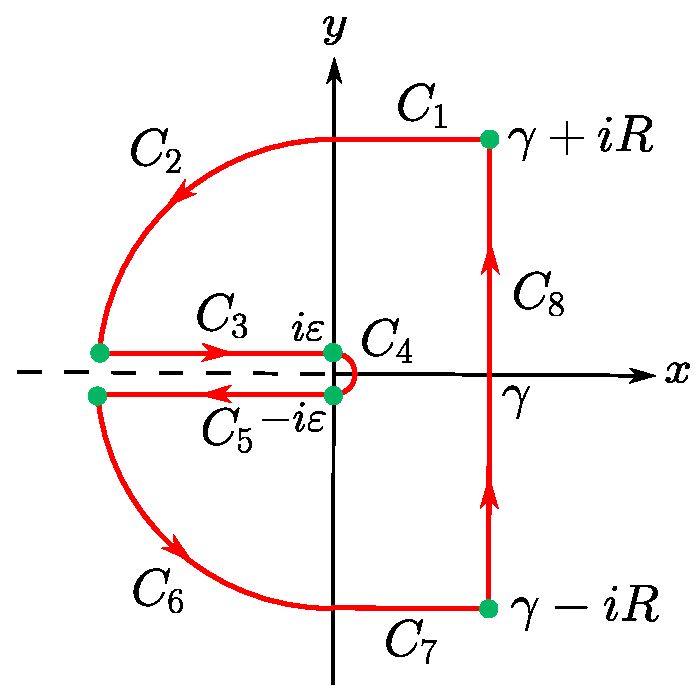
\includegraphics[scale = 0.6]{Figuras/InversaLaplace2.pdf}
        \caption{Contorno de integración para la transformada inversa de Laplace $1/\sqrt{s}$.}
        \label{fig:InvLaplaceBranchCut}
    \end{figure}

    Como el integrando es analítico en el interior del contorno cerrado, por el teorema de Cauchy-Goursat,
    $$\sum_{k=1}^{8} \int_{C_k} e^{st} \frac{1}{\sqrt{s}} \,ds = 0.$$

    Mostremos que la integral en torno a $C_1: s = x + i R, 0\leq x \leq \gamma$, se desvanece cuando $R \to \infty$. 

    Para $s \in C_1$, tenemos que
    $$\left|e^{st} \frac{1}{\sqrt{s}} \right| = \frac{e^{\real(s) t}}{\sqrt{|s|}} \leq \frac{e^{\gamma t}}{\sqrt{R}}.$$

    Luego,
    $$\left|\int_{C_1} e^{st} \frac{1}{\sqrt{s}} \,ds \right| \leq \int_0^{\gamma} \frac{e^{\gamma t}}{\sqrt{R}} \,dx = \frac{\gamma e^{\gamma t}}{\sqrt{R}} \overset{R \to \infty}{\longrightarrow} 0.$$

    Similarmente, se prueba que la integral en torno a $C_7: s = x - i R, 0 \leq x \leq \gamma$, se desvanece cuando $R \to \infty$.

    Ahora, mostremos que la integral en torno a $C_2: s = Re^{i\theta}, \pi/2 \leq \theta < \pi$, se desvanece cuando $R \to \infty$. 

     Para $s \in C_2$, tenemos que
    $$\left|e^{st} \frac{1}{\sqrt{s}} \right| = \frac{e^{\real(s) t}}{\sqrt{|s|}} = e^{R t \cos \theta }\frac{1}{\sqrt{R}}.$$

    Luego,
    $$\left|\int_{C_2} e^{st} \frac{1}{\sqrt{s}} \,ds \right| \leq \frac{1}{\sqrt{R}} \int_{\pi/2}^{\pi} e^{Rt \cos \theta} d\theta.$$

    Haciendo la sustitución $\phi = \theta - (\pi/2) \Rightarrow d\phi = d\theta$, en la integral y usando la desigualdad de Jordan, obtenemos
    $$\left|\int_{C_2} e^{st} \frac{1}{\sqrt{s}} \,ds \right| \leq \frac{1}{\sqrt{R}} \int_{0}^{\pi/2} e^{-Rt \sin \phi} d\phi \leq \frac{1}{\sqrt{R}} \frac{\pi}{2 R t}\overset{R \to \infty}{\longrightarrow} 0.$$

    Similarmente, se prueba que la integral en torno a $C_6$ se desvanece.

    Podemos mostrar que la integral en torno a $C_4: s = \varepsilon e^{i\theta}, -\pi/2 \leq \theta \leq \pi/2$, se desvanece cuando $\varepsilon \to 0$.

    Para $s \in C_4$, tenemos que
    $$\left|e^{st} \frac{1}{\sqrt{s}} \right| = \frac{e^{\real(s) t}}{\sqrt{|s|}} = \frac{e^{\varepsilon t \cos\theta}}{\sqrt{\varepsilon}} \leq  \frac{e^{\varepsilon t}}{\sqrt{\varepsilon}}.$$

    Luego,
    $$\left|\int_{C_4} e^{st} \frac{1}{\sqrt{s}} \,ds \right| \leq \frac{e^{\varepsilon t}}{\sqrt{\varepsilon}} \int_{-\pi/2}^{ \pi/2} \varepsilon d\theta = \frac{e^{\varepsilon t}}{\sqrt{\varepsilon}} (\pi \varepsilon) \overset{\varepsilon \to 0}{\longrightarrow} 0.$$

    Entonces,
    $$\int_{C_3} e^{st} \frac{1}{\sqrt{s}} \,ds + \int_{C_5} e^{st} \frac{1}{\sqrt{s}} \,ds + \int_{C_8} e^{st} \frac{1}{\sqrt{s}} \,ds = 0.$$

    Tomando el límite $R \to \infty$ y $\varepsilon \to 0$, podemos expresar la transformada inversa de Laplace como
    $$\mathcal{L}^{-1}\left\{ \frac{1}{\sqrt{s}}\right\} = \frac{1}{2\pi i} \int_{\gamma - i\infty}^{\gamma + i \infty} e^{st} \frac{1}{\sqrt{s}} \,ds = - \frac{1}{2\pi i} \lim_{R\to\infty}  \lim_{\varepsilon \to 0} \left[ \int_{C_3} e^{st} \frac{1}{\sqrt{s}} \,ds +  \int_{C_5} e^{st} \frac{1}{\sqrt{s}} \,ds\right].$$

    Bajo estos límites, tenemos que en $C_3$, $s = x$, $ds = dx$, con $x$ desde $-\infty$ a $0$, y en $C_5$, $s = x$, $ds = dx$, con $x$ desde $0$ a $-\infty$.  Luego,
    \begin{align*}
       \mathcal{L}^{-1}\left\{ \frac{1}{\sqrt{s}}\right\} &= - \frac{1}{2\pi i} \int_{-\infty}^0 e^{xt} \frac{e^{-i\pi/2}}{\sqrt{-x}} \,dx - \frac{1}{2\pi i} \int_0^{-\infty} e^{xt} \frac{e^{i\pi/2}}{\sqrt{-x}} \,dx \\
       &= -\frac{1}{2\pi} \int_{\infty}^0 e^{-xt} \frac{1}{\sqrt{x}} \,dx + \frac{1}{2\pi} \int_0^{\infty} e^{-xt} \frac{1}{\sqrt{x}} \,dx \\
       &= \frac{1}{\pi} \int_0^{\infty} e^{-xt} \frac{1}{\sqrt{x}} \,dx.
    \end{align*}

    Haciendo la sustitución $u = xt \Rightarrow du = t dx$,
    $$ \mathcal{L}^{-1}\left\{ \frac{1}{\sqrt{s}}\right\}  = \frac{1}{\pi \sqrt{t}} \int_0^{\infty} e^{-u} \frac{1}{\sqrt{u}} \,du.$$

    Pero,
    $$\int_0^{\infty} e^{-u} \frac{1}{\sqrt{u}} \,du = \Gamma\left( \frac{1}{2}\right) = \sqrt{\pi}.$$

    Por lo tanto,
    $$ \mathcal{L}^{-1}\left\{ \frac{1}{\sqrt{s}}\right\} = \frac{1}{\sqrt{\pi t}}, \quad t > 0.$$
\end{ejemplo}

\section{Propiedades de la transformada de Laplace}    

\begin{teorema}
    Si $f$ y $g$ son funciones cuyas transformadas de Laplace existen para $\real(s) > \alpha$ y sean $a, b \in \mathbb{R}$. Entonces, 
\begin{enumerate}
    \item \textbf{Linealidad:} Para $\real(s) > \alpha$,
    $$\mathcal{L}\{a f(t) + b g(t)\} = a \mathcal{L}\{f(t)\} + b \mathcal{L}\{g(t)\}.$$ 

    \item \textbf{Escalonamiento:} Para $\real(s) > \alpha \cdot \beta$,
    $$\mathcal{L}\{f(\beta t) \} = \frac{1}{\beta} F \left( \frac{s}{\beta}\right), \quad \beta > 0.$$ 
    
    \item \textbf{Desplazamiento en el plano $s$:} Para $\real(s) > \alpha + a$,
    $$\mathcal{L}\{e^{at} f(t)\} = F(s-a).$$
\end{enumerate}
\end{teorema}

\begin{ejemplo}
    Determine la transformada de Laplace de $e^{at} \sin(bt)$.

    \textbf{Solución:} En la primera sección, vimos que
    $$\mathcal{L}\{\sin(bt)\} = F(s) = \frac{b}{s^2+b^2}, \quad \real(s) > 0.$$

    Luego, por la propiedad de desplazamiento,
    $$\mathcal{L}\{e^{at} \sin(bt)\} = F(s-a) = \frac{b}{(s-a)^2+b^2}, \quad \real(s) > a.$$
\end{ejemplo}

\begin{teorema}[Propiedad de la derivada]
    Sea $f$ continua en $]0, + \infty [$ y $f'(t)$ continua por tramos en $[0, + \infty[$, ambas de orden exponencial $\alpha$. Entonces, para $\real(s) > \alpha$,
    $$\mathcal{L}\{f'(t)\} = s \mathcal{L}\{f(t)\} - f(0^+),$$

    donde $f(0^+) = \lim\limits_{t \to 0^+} f(t)$. 
\end{teorema}

En general, la transformada de Laplace de derivadas de orden superior están dadas por el siguiente teorema.

\begin{teorema}[Transformada de Laplace de derivadas de orden superior]
 Sean $f, f', \dots, f^{(n-1)}$ continuas para todo $t>0$ y sea $f^{(n)}$ continua por tramos en $[0,+\infty[$, con todas estas funciones de orden exponencial $\alpha$. Entonces, para $\real(s) > \alpha$,
$$\mathcal{L}\{f^{(n)}(t)\} = s^n \mathcal{L}\{f(t)\} - s^{n-1} f(0^+) - s^{n-2} f'(0^+) - \cdots - f^{(n-1)}(0^+). \label{LaplaceDerivada}$$

\end{teorema}

\begin{ejemplo}
Calcule 
$$\mathcal{L}\left\{\sin^2(at)\right\}.$$   

\textbf{Solución:} Sea $f(t) = \sin^2(at)$, entonces
$$f'(t) = 2a \sin(at) \cos(at) = a \sin(2at).$$

Como $f(0) = 0$ y $\frac{2a^2}{s^2+4a^2} = \mathcal{L}\{f'(t)\} = s \mathcal{L}\{f(t)\} - f(0)$, obtenemos
$$\mathcal{L}\left\{\sin^2(at)\right\} = \frac{2a^2}{s(s^2+4a^2)}, \quad \real(s) > 0.$$
\end{ejemplo}

Hemos determinando la transformada de Laplace de la derivada de una función $f$, es natural preguntarse sobre la transformada de una función definida por una integral:
$$g(t) = \int_0^t f(t') \,dt'.$$

\begin{teorema}
     Sea la función $f(t)$ continua por tramos y de orden exponencial $\alpha$. Entonces,
     $$\mathcal{L} \left\{ \int_0^t f(t') \,dt'\right\} = \frac{1}{s} \mathcal{L}\{f(t)\}, \quad \real(s) > \alpha.$$
\end{teorema}

\begin{demo}
Caso particular del teorema \ref{Teo:Convolucion} para 
$$(f * g)(t) = \int_0^t f(u) g(t-u) \,du,$$

con $g(t) = 1$.
\end{demo}

Para funciones periódicas, tenemos el siguiente teorema.

\begin{teorema}
 Sea $f$ una función continua por tramos en el intervalo $[0,T]$ y periódica con periodo $T>0$. Entonces $f$ tiene transformada de Laplace dada por
\begin{equation*}
\mathcal{L}\{f(t)\} = \frac{\int_0^T e^{-st} f(t) dt}{1-e^{-Ts}}, \quad \real(s) > 0.
\end{equation*}
   
\end{teorema}

\begin{ejemplo}
    Encuentre la transformada de Laplace de
    $$f(t) = \left\{ \begin{array}{cl}
     1,& \text{si} ~ 0 \leq t < \pi  \\
     0,& \text{si} ~ \pi \leq t < 2\pi
    \end{array} \right.$$

    y $f(t+ 2\pi) = f(t)$ para $t > 0$, ésto es, $f(t)$ es periódica para $t > 0$.

    \textbf{Solución:} Como $f$ es periódica de periodo $T = 2\pi$, tenemos que
    \begin{align*}
        \mathcal{L}\{f(t)\} &= \frac{\int_0^{2\pi} e^{-st} f(t) \,dt}{1-e^{-2\pi s}} \\
        &= \frac{\int_0^{\pi} e^{-st}\,dt}{1-e^{-2\pi s}} \\
        &= \frac{1-e^{-\pi s}}{s(1-e^{-2\pi s})} \\
        &= \frac{1}{s(1+e^{-\pi s})}.
    \end{align*}
\end{ejemplo}

\begin{teorema}[Integral de una transformada]
   Si $\int_0^{\beta} \frac{f(t)}{t} \,dt$ existe para $\beta > 0$ y $f(t)$ es de orden exponencial $\alpha$, entonces
   $$\mathcal{L}\left\{\frac{f(t)}{t}\right\} = \int_s^{\infty} F(u) \,du, \quad s > \alpha.$$
\end{teorema}

\section{Convolución}

\begin{defi}
   Sean $f$ y $g$ funciones continuas por tramos en $[0, \infty[$. La \textbf{convolución} de $f$ y $g$, que se denota $f*g$, se define como
\begin{equation*}
(f*g)(t) := \int_0^t f(t-u)g(u) \, du.
\end{equation*}  
\end{defi}

Es claro que la convolución es distinta de la multiplicación común. Por ejemplo, $1*1 = t \neq 1$, y en general, $1*f \neq f$. Sin embargo, la convolución sí satisface algunas propiedades de la multiplicación.

\begin{teorema}[Propiedades de la convolución]
Sean $f$, $g$ y $h$ continuas por tramos en $[0,  \infty[$. Entonces,

\begin{itemize}
\item[(i)] $f*g = g*f$,

\item[(ii)] $f*(g*h) = (f*g)*h$,  

\item[(iii)] $f*(g+h) = f*g + f*h$. 
\end{itemize} 
\end{teorema}

Al igual que para la transformada de Fourier, la transformada de Laplace de la convolución obedece el siguiente teorema.

\begin{teorema}[de Convolución] \label{Teo:Convolucion}
    Sean $f$ y $g$ funciones continuas por tramos, de orden exponencial, tales que:
    \begin{equation*}
    \mathcal{L}\{f(t)\} = F(s) ~~\mbox{y}~~ \mathcal{L}\{g(t)\} = G(s),
    \end{equation*}

    entonces
    \begin{equation*}
    \mathcal{L}\{(f*g)(t)\} = F(s)G(s),
    \end{equation*}

    o, de manera equivalente,
    \begin{equation*}
    \mathcal{L}^{-1}\{F(s)G(s)\}(t) = (f*g)(t).
    \end{equation*}    
\end{teorema}

\begin{demo}

Tomando la transformada de Laplace de la convolución $f * g$,
$$\mathcal{L}\{(f*g)(t)\} = \int_0^{\infty} e^{-st} \int_0^t f(t-u) g(u) \,du \,dt = \int_0^{\infty} \int_0^t e^{-st}  f(t-u) g(u) \,du \,dt.$$

La región de integración se ilustra en la figura \ref{fig:Convolucion2}.

\begin{figure}[H]
    \centering
    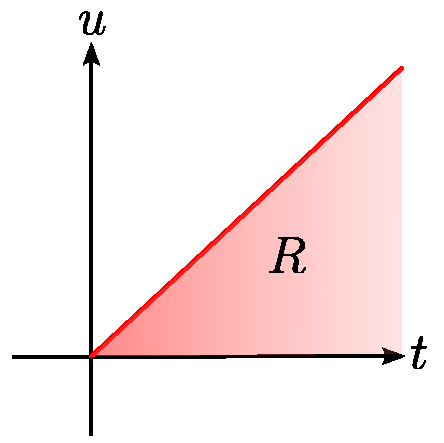
\includegraphics[scale = 0.6]{Figuras/Laplace-Convolucion-2.pdf}
    \caption{Región de integración.}
    \label{fig:Convolucion2}
\end{figure}

Luego, haciendo un cambio en el orden de integración, se tiene
$$\mathcal{L}\{(f*g)(t)\} = \int_0^{\infty} \int_u^{\infty} e^{-st} f(t-u) g(u) \,dt\,du.$$

Si hacemos el cambio de variable $v = t-u$ en la integral interior, obtenemos que
\begin{align*}
    \mathcal{L}\{(f*g)(t)\} &= \int_0^{\infty} g(u) \int_0^{\infty} e^{-s(u+v)} f(v) \,dv \,du \\
    &= \left(\int_0^{\infty} g(u) e^{-su} du \right)\left(\int_0^{\infty} f(v) e^{-sv} \,dv  \right) \\
    &= F(s)G(s). 
\end{align*}

\end{demo}

\begin{ejemplo}
Calcule
$$\mathcal{L}^{-1} \left\{ \frac{s}{(s^2+1)^2} \right\}.$$

\textbf{Solución:} Notemos que 
\begin{equation*}
\mathcal{L}^{-1} \left\{ \frac{s}{(s^2+1)^2} \right\} = \mathcal{L}^{-1} \left\{ \frac{s}{s^2+1} \cdot \frac{1}{s^2+1} \right\}.
\end{equation*}

Como
\begin{equation*}
\mathcal{L}\{\cos(t)\} = \frac{s}{s^2+1} ~~\mbox{y}~~ \mathcal{L}\{\sin(t)\} = \frac{1}{s^2+1},
\end{equation*}

tenemos, por el teorema de convolución, que
\begin{align*}
    \mathcal{L}^{-1} \left\{ \frac{s}{(s^2+1)^2} \right\} &=\cos(t) *\sin(t)  \\
    &= \int_0^t \sin(t-u) \cos(u) \,du \\
    &= \int_0^t (\sin(t) \cos(u) - \cos(u) \sin(u)) \cos(u) \,du  \\
    &= \sin(t) \int_0^t \cos^2(u) \,du - \cos(t) \int_0^t \sin (u) \cos(u) \,du \\
    &= \sin(t) \left[ \frac{1}{2} u + \frac{\sin(2u)}{4} \right]_0^t - \cos(t) \left[ \frac{\sin^2(u)}{2} \right]_0^t \\
    &= \frac{t \sin(t)}{2} + \frac{\sin(2t)}{4} \sin(t) - \cos(t) \frac{\sin^2(t)}{2} \\
    &= \frac{t \sin(t) }{2}.
\end{align*}

Por lo tanto,
$$\mathcal{L}^{-1} \left\{ \frac{s}{(s^2+1)^2} \right\} = \frac{t \sin(t) }{2}.$$   
\end{ejemplo}

\section{Aplicaciones de la transformada de Laplace}

La transformada de Laplace, al igual que la transformada de Fourier, nos permite convertir ecuaciones diferenciales en ecuaciones algebraicas, con una diferencia: se requiere el valor de la función en un punto dado. Lo anterior nos entrega una ligera ventaja y es que una vez que se invierta la transformada, tendremos de inmediato la solución al problema, recalcando que el dominio de validez de la función encontrada es para $t > 0$. Otra diferencia relevante es que, mientras la transformada de Fourier sólo se puede aplicar a funciones que decrecen rápidamente a cero, la transformada de Laplace está bien definida incluso para funciones de crecimiento exponencial. Entonces, si estamos en presencia de un sistema físico caracterizado por una variable que crece exponencialmente, es bastante probable que la transformada de Fourier dé resultados sin sentido físico.

A continuación expondremos tres situaciones, en las cuales el uso de la transformada de Laplace es ventajoso.

\subsection{Ecuaciones diferenciales lineales con coeficientes constantes}

\begin{ejemplo}
    Consideremos la ecuación diferencial
    $$y'(t) + y(t) = \cos(t), \quad \text{para} ~ t > 0, \quad y(0) = 1.$$

    Apliquemos la transformada de Laplace a ambos lados de la ecuación:
    $$\mathcal{L}\{y'(t)\} - \mathcal{L}\{y(t)\} = \mathcal{L}\{\cos(t)\}.$$

    Evaluamos la transformada de la primera derivada, usando los teoremas enunciados durante el capítulo.
    $$\mathcal{L}\{y'(t)\} = s Y(s) - y(0) = s Y(s) - 1,$$

    donde $Y(s) = \mathcal{L}\{y(t)\}$. Luego, la ecuación diferencial nos queda:
    \begin{align*}
        sY(s) - 1 + Y(s) &= \frac{s}{s^2+1} \\
        \Rightarrow \quad Y(s) &= \frac{s}{(s+1)(s^2+1)} + \frac{1}{s+1} \\
        \Rightarrow \quad Y(s) &= \frac{1/2}{s+1} + \frac{1}{2} \frac{s+1}{s^2+1}.
    \end{align*}

    Aplicando la transformada de Laplace inversa,
    $$y(t) = \frac{1}{2} e^{-t} + \frac{1}{2} \cos(t) + \frac{1}{2} \sin(t), \quad t > 0.$$
\end{ejemplo}

\subsection{Ecuaciones integrales}

Una \textbf{ecuación integral} es aquella ecuación donde la función incógnita $\varphi(x)$ se encuentra dentro de una integral. Estas ecuaciones integrales se clasifican en dos formas \cite{Arfken}:
\begin{itemize}
    \item Si los límites de integración están fijos, llamamos la ecuación una \textbf{ecuación de Fredholm}; si un límite es variable, es una \textbf{ecuación de Volterra}.

    \item Si la función incógnita aparece solo en la integral, la etiquetamos como de \textbf{primera especie}. Si aparece tanto dentro como fuera de la integral, la etiquetemos como de \textbf{segunda especie}.
\end{itemize}

A continuación algunos ejemplos de estas definiciones donde $\varphi(t)$ es la función desconocida, $K(x,t)$ una función de dos variables que la llamaremos \textbf{kernel}, y $f(x)$ una función que asumimos conocida.

\begin{enumerate}
    \item \textbf{Ecuación de Fredholm de primera especie}:
    $$f(x) = \int_a^b K(x,t) \varphi(t) \,dt.$$

    \item \textbf{Ecuación de Fredholm de segunda especie}:
    $$\varphi(x) = f(x) + \lambda \int_a^b K(x,t) \varphi(t) \,dt.$$

    \item \textbf{Ecuación de Volterra de primera especie}:
    $$f(x) = \int_a^x K(x,t) \varphi(t) \,dt.$$

    \item \textbf{Ecuación de Volterra de segunda especie}:
    $$\varphi(x) = f(x) + \int_a^x K(x,t) \varphi(t) \,dt.$$
\end{enumerate}

En esta sección nos enfocaremos en ecuaciones de Volterra para $K(x,t) = K(x-t)$, de tal forma que
$$\int_a^x K(x,t) \varphi(t) \,dt = (K * \varphi)(x).$$

Para ilustrar el método, consideremos la situación física planteada en el siguiente ejemplo.

\begin{ejemplo}[Problema de la tautócrona]
    Una partícula de masa $m$ resbala (parte del reposo), sin roce, sobre una curva bajo el efecto de la gravedad. Buscamos determinar la forma de la curva de modo que el tiempo que le toma a la partícula en llegar al suelo sea independiente del punto de lanzamiento. 

    \begin{figure}[H]
        \centering
        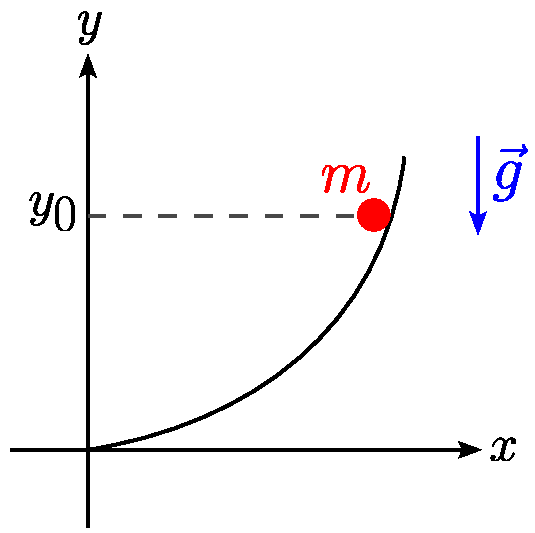
\includegraphics[scale = 0.65]{Figuras/tautocrona.pdf}
        \caption{Esquema de la situación física.}
        \label{fig:tautocrona}
    \end{figure}

    Como estamos en presencia de fuerzas conservativas, la  energía se conserva durante todo el trayecto para todo $y$, ésto es,
    \begin{alignat*}{3}
    &               &\quad   \text{Energía inicial en $y_0$} &= \text{Energía final en $y$} \\
    &  \Rightarrow  &\quad      mgy_0 &= \frac{1}{2} mv^2 + mgy \\
    &  \Rightarrow  &\quad   \frac{1}{2} mv^2 &= mg(y_0 - y) \\
    &  \Rightarrow  &\quad   v &= \sqrt{2 g} \sqrt{y_0-y}, 
    \end{alignat*}   
    
    donde $y_0$ es la altura inicial. El tiempo de descenso está dado por
    $$T(y_0) = \int \frac{ds}{v} = \int_{y_0}^0 \frac{1}{v} \frac{ds}{dy} dy = - \int_0^{y_0} f(y) (y_0 - y)^{-1/2} \frac{1}{\sqrt{2g}} dy,$$

    donde $f(y) = ds/dy$. Ahora, si suponemos que $T(y_0)$ es constante $T_0$, ésto es, independiente del punto de partida $y_0$. La condición queda
    $$\int_0^{y_0} f(y) (y_0 - y)^{-1/2} \,dy = C_0,$$

    donde $C_0 = -\sqrt{2g} T_0$. Aplicando la transformada de Laplace  a ambos lados de la ecuación:
    $$\mathcal{L}\left\{\int_0^{y_0} f(y) (y_0 - y)^{-1/2} \,dy \right\} = \mathcal{L}\{C_0\} = \frac{C_0}{s}.$$
    
    Por el teorema de convolución, tenemos que
    $$\mathcal{L}\{f(y)\} \mathcal{L}\{y^{-1/2}\} = \frac{C_0}{s} \Rightarrow \mathcal{L}\{f(y)\} = \frac{C_0/s}{\mathcal{L}\{y^{-1/2}\}}.$$

    Pero,
    $$\mathcal{L}\{y^{-1/2}\} = \int_0^{\infty} e^{-sy} \frac{1}{\sqrt{y}} \,dy \overset{\textcolor{blue}{t = sy}}{=} \frac{1}{\sqrt{s}}\int_0^{\infty} e^{-t} \frac{1}{\sqrt{t}} \,dt = \frac{\Gamma\left(\frac{1}{2}\right)}{\sqrt{s}}.$$

    Así,
    $$\mathcal{L}\{f(y)\} = \frac{C_0}{s} \frac{\sqrt{s}}{\Gamma\left(\frac{1}{2}\right)} = \frac{C_0}{\sqrt{\pi}} \frac{1}{\sqrt{s}}.$$

    Tomando la transformada inversando y usando el resultado del ejemplo \ref{Inv_Laplace_ej_branch}, obtenemos 
    $$f(y) = \frac{C_0}{\pi} \frac{1}{\sqrt{y}} = \frac{C}{\sqrt{y}},$$

    donde $C = C_0/\pi$. Recordando que $f(y) = ds/dy$, notemos que
    \begin{align*}
        ds^2 = dx^2 + dy^2 &\Rightarrow dx = \sqrt{ds^2 - dy^2} \\
        &\Rightarrow dx = \sqrt{\left( \frac{ds}{dy} dy\right)^2 - dy^2} \\
        &\Rightarrow dx = \sqrt{\left(\frac{ds}{dy}\right)^2 - 1} \,dy \\
        &\Rightarrow \frac{dx}{dy} = \sqrt{\frac{C^2}{y} - 1}. 
    \end{align*}

    Integrando con respecto a $y$,
    $$x(y) = \int \sqrt{\frac{C^2}{y} - 1} \,dy.$$

    Haciendo el cambio de variable $y = C^2 \sin^2 (\phi) \Rightarrow dy = 2 C^2 \sin(\phi) \cos(\phi) \,d\phi$,
    \begin{align*}
        x &= \int \sqrt{\csc^2(\phi) - 1} \, 2 C^2 \sin(\phi) \cos(\phi) \,d\phi \\
        &= 2C^2 \int \sqrt{\cot^2(\phi)}  \sin(\phi) \cos(\phi) \,d\phi \\
        &= 2C^2 \int \cos^2(\phi) \,d\phi \\
        &=  \frac{C^2}{2} (2\phi + \sin(2\phi)) + D,
    \end{align*}

    donde $D$ es una constante de integración. Entonces,
    \begin{align*}
        x &= \frac{C^2}{2} (2\phi + \sin(2\phi)) + D, \\
        y &= \frac{C^2}{2} (1 - \cos(2\phi)).
    \end{align*}

    La curva debe pasar por el origen $(0,0)$, así que $D = 0$, y si definimos un nuevo parámetro $\theta = 2\phi$, encontramos que
    \begin{align*}
        x &= \frac{C^2}{2} (\theta + \sin(\theta)), \\
        y &= \frac{C^2}{2} (1 - \cos(\theta)).
    \end{align*}

    Estas son las ecuaciones paramétricas de un cicloide.
\end{ejemplo}

\subsection{Sistema de ecuaciones lineales}

La transformada de Laplace puede ser usada para convertir un sistema de ecuaciones diferenciales con coeficientes constantes en un sistema de ecuaciones algebraicas. 

\begin{ejemplo}
    Consideremos el circuito de la figura \ref{fig:Circuit}. 
    
    \begin{figure}[H]
        \centering
        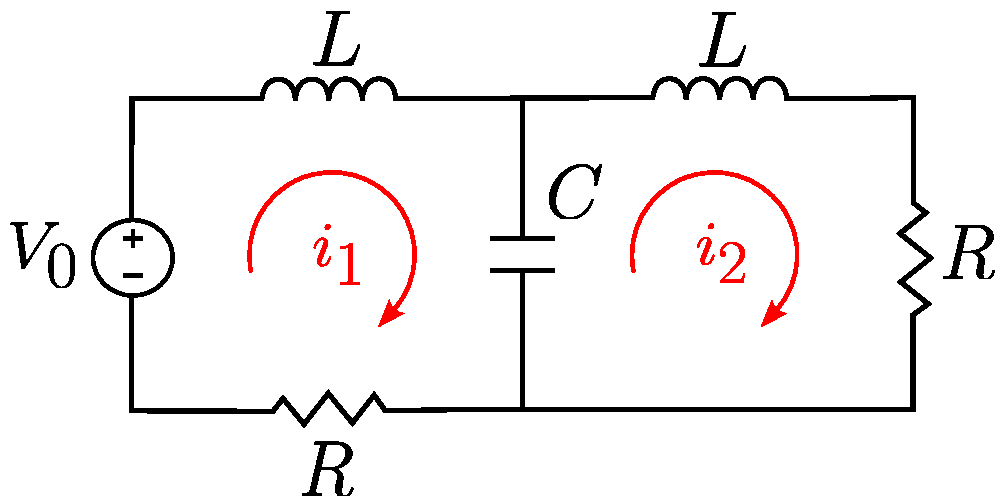
\includegraphics[scale = 0.65]{Figuras/Circuito.pdf}
        \caption{Circuito eléctrico.}
        \label{fig:Circuit}
    \end{figure}
    
    Usando las leyes de Kirchhoff, encontramos el siguiente sistema de ecuaciones diferenciales.
    \begin{align*}
        L \frac{di_1}{dt} + Ri_1 + \frac{q}{C} &= V_0, \\
        L \frac{di_2}{dt} + Ri_2 - \frac{q}{C} &= 0, \\
        \frac{dq}{dt} &= i_1 - i_2.
    \end{align*}
    
    Inicialmente el capacitador se encuentra descargado y las corrientes inducidas por las inductancias son despreciables de tal forma que se tienen las condiciones iniciales:
    $$i_1(0) = i_2(0) = \frac{V_0}{2R}, \quad q(0) = 0.$$

    Aplicamos la transformada de Laplace al sistema de ecuaciones diferenciales.
    \begin{align*}
        L\left( sI_1(s) - \frac{V_0}{2R} \right) + RI_1(s) + \frac{Q(s)}{C} &= \frac{V_0}{s}, \\
       L\left( sI_2(s) - \frac{V_0}{2R} \right) + RI_2(s) - \frac{Q(s)}{C}  &= 0, \\
        sQ(s) &= I_1(s) - I_2(s),
    \end{align*}

    donde $I_1(s) = \mathcal{L}\{i_1(t)\}$, $I_2(s) = \mathcal{L}\{i_2(t)\}$ y $Q(s) = \mathcal{L}\{q(t)\}$. Despejando estas cantidades:
    \begin{align*}
        I_1 &= \frac{V_0}{2} \left(\frac{1}{Rs} + \frac{1/L}{s^2 + R s/L + 2/(CL)} \right) \\
        I_2 &= \frac{V_0}{2} \left(\frac{1}{Rs} - \frac{1/L}{s^2 + R s/L + 2/(CL)} \right) \\
            Q &= \frac{C V_0}{2} \left( \frac{1}{s} - \frac{s+R/L}{s^2 + Rs/L + 2/(CL)} \right)
    \end{align*}

    Factorizando las polinomios de los denominadores.
    \begin{align*}
        I_1 &= \frac{V_0}{2} \left(\frac{1}{Rs} + \frac{1/L}{(s+\alpha - i \omega)(s + \alpha + i \omega)} \right) \\
        I_2 &= \frac{V_0}{2} \left(\frac{1}{Rs} - \frac{1/L}{(s+\alpha - i\omega)(s+\alpha + i \omega)} \right) \\
        Q &= \frac{C V_0}{2} \left( \frac{1}{s} - \frac{s+2\alpha}{(s+\alpha - i\omega)(s+\alpha + i \omega))} \right).
    \end{align*}

    Aquí hemos definido
    $$\alpha = \frac{R}{2L} \quad \text{y} \quad \omega^2 = \frac{2}{LC} - \alpha^2.$$

    Expandiendo las funciones en fracciones parciales.
    \begin{align*}
        I_1 &= \frac{V_0}{2} \left(\frac{1}{Rs} + \frac{i}{2\omega L} \left(\frac{1}{s+\alpha + i\omega} - \frac{1}{s+\alpha - i\omega} \right) \right) \\
        I_2 &= \frac{V_0}{2} \left(\frac{1}{Rs} - \frac{i}{2\omega L} \left(\frac{1}{s+\alpha + i\omega} - \frac{1}{s+\alpha - i\omega} \right) \right) \\
        Q &= \frac{C V_0}{2} \left( \frac{1}{s} + \frac{i}{2\omega} \left( \frac{\alpha + i\omega}{s+\alpha - i\omega} - \frac{\alpha - i \omega}{s+\alpha +i\Omega} \right) \right).
    \end{align*}

    Ahora, aplicamos la transformada inversa, teniendo en consideración que
    $$\mathcal{L}^{-1}\left\{ \frac{1}{s-a} \right\} = e^{at},$$
     \begin{align*}
        i_1 &= \frac{V_0}{2} \left(\frac{1}{R} + \frac{i}{2\omega L} \left( e^{(-\alpha - i\omega)t} - e^{(-\alpha + i\omega)t}\right) \right) \\
        i_2 &= \frac{V_0}{2} \left(\frac{1}{R} - \frac{i}{2\omega L} \left( e^{(-\alpha - i\omega)t} - e^{(-\alpha + i \omega)t}\right) \right) \\
        q &= \frac{C V_0}{2} \left( 1 + \frac{i}{2\omega} \left( (\alpha + i\omega) e^{(-\alpha + i \omega)t} - (\alpha - i\omega)e^{(-\alpha - i\omega)t} \right) \right).
    \end{align*}

    Simplicando las expresiones, obtenemos las soluciones.
    \begin{align*}
        i_1 &= \frac{V_0}{2} \left(\frac{1}{R} + \frac{1}{\omega L} e^{-\alpha t}\sin(\omega t) \right), \\
        i_2 &= \frac{V_0}{2} \left(\frac{1}{R} - \frac{1}{\omega L} e^{-\alpha t}\sin(\omega t) \right), \\
        q &= \frac{CV_0}{2} \left( 1- e^{-\alpha t} \left( \cos(\omega t) + \frac{\alpha}{\omega} \sin(\omega t) \right)\right).
    \end{align*}
\end{ejemplo}








 


\nocite{*} %Referencia todo, incluso lo que no está citado.
\printbibliography[title={Referencias}]

\end{document}
